% Options for packages loaded elsewhere
\PassOptionsToPackage{unicode}{hyperref}
\PassOptionsToPackage{hyphens}{url}
%
\documentclass[
]{book}
\usepackage{amsmath,amssymb}
\usepackage{lmodern}
\usepackage{iftex}
\ifPDFTeX
  \usepackage[T1]{fontenc}
  \usepackage[utf8]{inputenc}
  \usepackage{textcomp} % provide euro and other symbols
\else % if luatex or xetex
  \usepackage{unicode-math}
  \defaultfontfeatures{Scale=MatchLowercase}
  \defaultfontfeatures[\rmfamily]{Ligatures=TeX,Scale=1}
\fi
% Use upquote if available, for straight quotes in verbatim environments
\IfFileExists{upquote.sty}{\usepackage{upquote}}{}
\IfFileExists{microtype.sty}{% use microtype if available
  \usepackage[]{microtype}
  \UseMicrotypeSet[protrusion]{basicmath} % disable protrusion for tt fonts
}{}
\makeatletter
\@ifundefined{KOMAClassName}{% if non-KOMA class
  \IfFileExists{parskip.sty}{%
    \usepackage{parskip}
  }{% else
    \setlength{\parindent}{0pt}
    \setlength{\parskip}{6pt plus 2pt minus 1pt}}
}{% if KOMA class
  \KOMAoptions{parskip=half}}
\makeatother
\usepackage{xcolor}
\IfFileExists{xurl.sty}{\usepackage{xurl}}{} % add URL line breaks if available
\IfFileExists{bookmark.sty}{\usepackage{bookmark}}{\usepackage{hyperref}}
\hypersetup{
  pdftitle={INTRODUCCIÓN A SERIES DE TIEMPO},
  pdfauthor={LUIS ORTIZ-CEVALLOS},
  hidelinks,
  pdfcreator={LaTeX via pandoc}}
\urlstyle{same} % disable monospaced font for URLs
\usepackage{color}
\usepackage{fancyvrb}
\newcommand{\VerbBar}{|}
\newcommand{\VERB}{\Verb[commandchars=\\\{\}]}
\DefineVerbatimEnvironment{Highlighting}{Verbatim}{commandchars=\\\{\}}
% Add ',fontsize=\small' for more characters per line
\usepackage{framed}
\definecolor{shadecolor}{RGB}{248,248,248}
\newenvironment{Shaded}{\begin{snugshade}}{\end{snugshade}}
\newcommand{\AlertTok}[1]{\textcolor[rgb]{0.94,0.16,0.16}{#1}}
\newcommand{\AnnotationTok}[1]{\textcolor[rgb]{0.56,0.35,0.01}{\textbf{\textit{#1}}}}
\newcommand{\AttributeTok}[1]{\textcolor[rgb]{0.77,0.63,0.00}{#1}}
\newcommand{\BaseNTok}[1]{\textcolor[rgb]{0.00,0.00,0.81}{#1}}
\newcommand{\BuiltInTok}[1]{#1}
\newcommand{\CharTok}[1]{\textcolor[rgb]{0.31,0.60,0.02}{#1}}
\newcommand{\CommentTok}[1]{\textcolor[rgb]{0.56,0.35,0.01}{\textit{#1}}}
\newcommand{\CommentVarTok}[1]{\textcolor[rgb]{0.56,0.35,0.01}{\textbf{\textit{#1}}}}
\newcommand{\ConstantTok}[1]{\textcolor[rgb]{0.00,0.00,0.00}{#1}}
\newcommand{\ControlFlowTok}[1]{\textcolor[rgb]{0.13,0.29,0.53}{\textbf{#1}}}
\newcommand{\DataTypeTok}[1]{\textcolor[rgb]{0.13,0.29,0.53}{#1}}
\newcommand{\DecValTok}[1]{\textcolor[rgb]{0.00,0.00,0.81}{#1}}
\newcommand{\DocumentationTok}[1]{\textcolor[rgb]{0.56,0.35,0.01}{\textbf{\textit{#1}}}}
\newcommand{\ErrorTok}[1]{\textcolor[rgb]{0.64,0.00,0.00}{\textbf{#1}}}
\newcommand{\ExtensionTok}[1]{#1}
\newcommand{\FloatTok}[1]{\textcolor[rgb]{0.00,0.00,0.81}{#1}}
\newcommand{\FunctionTok}[1]{\textcolor[rgb]{0.00,0.00,0.00}{#1}}
\newcommand{\ImportTok}[1]{#1}
\newcommand{\InformationTok}[1]{\textcolor[rgb]{0.56,0.35,0.01}{\textbf{\textit{#1}}}}
\newcommand{\KeywordTok}[1]{\textcolor[rgb]{0.13,0.29,0.53}{\textbf{#1}}}
\newcommand{\NormalTok}[1]{#1}
\newcommand{\OperatorTok}[1]{\textcolor[rgb]{0.81,0.36,0.00}{\textbf{#1}}}
\newcommand{\OtherTok}[1]{\textcolor[rgb]{0.56,0.35,0.01}{#1}}
\newcommand{\PreprocessorTok}[1]{\textcolor[rgb]{0.56,0.35,0.01}{\textit{#1}}}
\newcommand{\RegionMarkerTok}[1]{#1}
\newcommand{\SpecialCharTok}[1]{\textcolor[rgb]{0.00,0.00,0.00}{#1}}
\newcommand{\SpecialStringTok}[1]{\textcolor[rgb]{0.31,0.60,0.02}{#1}}
\newcommand{\StringTok}[1]{\textcolor[rgb]{0.31,0.60,0.02}{#1}}
\newcommand{\VariableTok}[1]{\textcolor[rgb]{0.00,0.00,0.00}{#1}}
\newcommand{\VerbatimStringTok}[1]{\textcolor[rgb]{0.31,0.60,0.02}{#1}}
\newcommand{\WarningTok}[1]{\textcolor[rgb]{0.56,0.35,0.01}{\textbf{\textit{#1}}}}
\usepackage{longtable,booktabs,array}
\usepackage{calc} % for calculating minipage widths
% Correct order of tables after \paragraph or \subparagraph
\usepackage{etoolbox}
\makeatletter
\patchcmd\longtable{\par}{\if@noskipsec\mbox{}\fi\par}{}{}
\makeatother
% Allow footnotes in longtable head/foot
\IfFileExists{footnotehyper.sty}{\usepackage{footnotehyper}}{\usepackage{footnote}}
\makesavenoteenv{longtable}
\usepackage{graphicx}
\makeatletter
\def\maxwidth{\ifdim\Gin@nat@width>\linewidth\linewidth\else\Gin@nat@width\fi}
\def\maxheight{\ifdim\Gin@nat@height>\textheight\textheight\else\Gin@nat@height\fi}
\makeatother
% Scale images if necessary, so that they will not overflow the page
% margins by default, and it is still possible to overwrite the defaults
% using explicit options in \includegraphics[width, height, ...]{}
\setkeys{Gin}{width=\maxwidth,height=\maxheight,keepaspectratio}
% Set default figure placement to htbp
\makeatletter
\def\fps@figure{htbp}
\makeatother
\setlength{\emergencystretch}{3em} % prevent overfull lines
\providecommand{\tightlist}{%
  \setlength{\itemsep}{0pt}\setlength{\parskip}{0pt}}
\setcounter{secnumdepth}{5}
\ifLuaTeX
  \usepackage{selnolig}  % disable illegal ligatures
\fi
\usepackage[]{natbib}
\bibliographystyle{apalike}

\title{INTRODUCCIÓN A SERIES DE TIEMPO}
\author{LUIS ORTIZ-CEVALLOS}
\date{2021-09-23}

\begin{document}
\maketitle

{
\setcounter{tocdepth}{1}
\tableofcontents
}
\hypertarget{quuxe9-es-una-de-serie-de-tiempo}{%
\chapter{¿Qué es una de serie de tiempo?}\label{quuxe9-es-una-de-serie-de-tiempo}}

\begin{Shaded}
\begin{Highlighting}[]
\FunctionTok{library}\NormalTok{(}\StringTok{"readr"}\NormalTok{)}
\FunctionTok{library}\NormalTok{(}\StringTok{"xts"}\NormalTok{) }
\FunctionTok{library}\NormalTok{(}\StringTok{"zoo"}\NormalTok{)}
\FunctionTok{library}\NormalTok{(}\StringTok{"astsa"}\NormalTok{)}
\FunctionTok{library}\NormalTok{(}\StringTok{"forecast"}\NormalTok{)}
\FunctionTok{library}\NormalTok{(}\StringTok{"ggplot2"}\NormalTok{)}
\FunctionTok{library}\NormalTok{(}\StringTok{"forecast"}\NormalTok{)}
\FunctionTok{library}\NormalTok{(}\StringTok{"ggfortify"}\NormalTok{)}
\FunctionTok{library}\NormalTok{(}\StringTok{"stargazer"}\NormalTok{)}
\FunctionTok{library}\NormalTok{(}\StringTok{"urca"}\NormalTok{)}
\FunctionTok{library}\NormalTok{(}\StringTok{"dynlm"}\NormalTok{)}
\FunctionTok{library}\NormalTok{(}\StringTok{"scales"}\NormalTok{)}
\FunctionTok{library}\NormalTok{(}\StringTok{"quantmod"}\NormalTok{)}
\NormalTok{TRIM}\OtherTok{\textless{}{-}}\FunctionTok{as.xts}\NormalTok{(}\FunctionTok{read.zoo}\NormalTok{(}\StringTok{"FINAL\_HN.csv"}\NormalTok{, }\AttributeTok{index.column =} \DecValTok{1}\NormalTok{, }\AttributeTok{sep =} \StringTok{";"}\NormalTok{, }\AttributeTok{header=}\ConstantTok{TRUE}\NormalTok{, }\AttributeTok{format =} \StringTok{"\%d/\%m/\%Y"}\NormalTok{))}
\NormalTok{MES}\OtherTok{\textless{}{-}}\FunctionTok{as.xts}\NormalTok{(}\FunctionTok{read.zoo}\NormalTok{(}\StringTok{"MES\_HN.csv"}\NormalTok{, }\AttributeTok{index.column =} \DecValTok{1}\NormalTok{, }\AttributeTok{sep =} \StringTok{";"}\NormalTok{, }\AttributeTok{header=}\ConstantTok{TRUE}\NormalTok{, }\AttributeTok{format =} \StringTok{"\%d/\%m/\%Y"}\NormalTok{))}
\NormalTok{IMAE}\OtherTok{\textless{}{-}}\NormalTok{MES}\SpecialCharTok{$}\NormalTok{IMAE}
\NormalTok{P}\OtherTok{\textless{}{-}}\NormalTok{ggplot2}\SpecialCharTok{::}\FunctionTok{autoplot}\NormalTok{(}\FunctionTok{log}\NormalTok{(IMAE))}\SpecialCharTok{+}\FunctionTok{xlab}\NormalTok{(}\StringTok{"Year"}\NormalTok{)}\SpecialCharTok{+}
\FunctionTok{ggtitle}\NormalTok{(}\StringTok{"LOGARITMO DEL IMAE EN HONDURAS"}\NormalTok{)}
\end{Highlighting}
\end{Shaded}

\begin{Shaded}
\begin{Highlighting}[]
\NormalTok{P}
\end{Highlighting}
\end{Shaded}

\includegraphics{index_files/figure-latex/unnamed-chunk-2-1.pdf}

\hypertarget{serie-ruido-blanco-wn}{%
\section{Serie Ruido Blanco (WN)}\label{serie-ruido-blanco-wn}}

\begin{Shaded}
\begin{Highlighting}[]
\NormalTok{X\_WN}\OtherTok{\textless{}{-}}\FunctionTok{arima.sim}\NormalTok{(}\FunctionTok{list}\NormalTok{(}\AttributeTok{order=}\FunctionTok{c}\NormalTok{(}\DecValTok{0}\NormalTok{,}\DecValTok{0}\NormalTok{,}\DecValTok{0}\NormalTok{)), }\AttributeTok{n=}\DecValTok{1000}\NormalTok{, }\AttributeTok{mean=}\DecValTok{4}\NormalTok{, }\AttributeTok{sd=}\DecValTok{2}\NormalTok{)}
\FunctionTok{autoplot}\NormalTok{(X\_WN)}\SpecialCharTok{+}
\FunctionTok{ggtitle}\NormalTok{(}\StringTok{"Serie Ruido Blanco"}\NormalTok{)}
\end{Highlighting}
\end{Shaded}

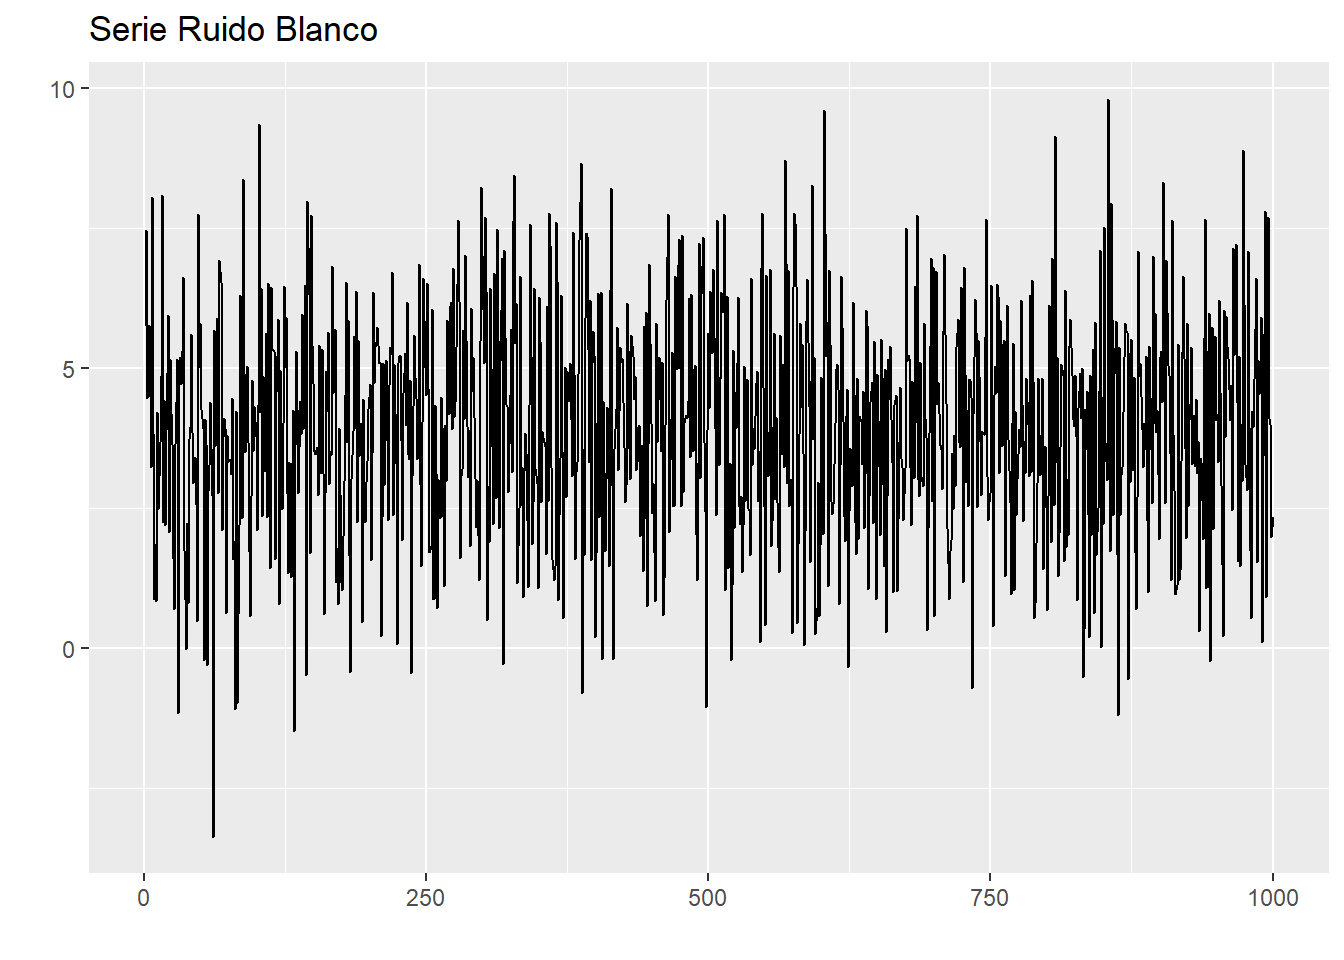
\includegraphics{index_files/figure-latex/unnamed-chunk-3-1.pdf}

\hypertarget{serie-random-walk-rw}{%
\section{Serie Random Walk (RW)}\label{serie-random-walk-rw}}

\begin{Shaded}
\begin{Highlighting}[]
\NormalTok{X\_RW}\OtherTok{\textless{}{-}}\FunctionTok{arima.sim}\NormalTok{(}\FunctionTok{list}\NormalTok{(}\AttributeTok{order=}\FunctionTok{c}\NormalTok{(}\DecValTok{0}\NormalTok{,}\DecValTok{1}\NormalTok{,}\DecValTok{0}\NormalTok{)), }\AttributeTok{n=}\DecValTok{100}\NormalTok{)}
\FunctionTok{autoplot}\NormalTok{(X\_RW)}\SpecialCharTok{+}
\FunctionTok{ggtitle}\NormalTok{(}\StringTok{"Serie Random Walk"}\NormalTok{)}
\end{Highlighting}
\end{Shaded}

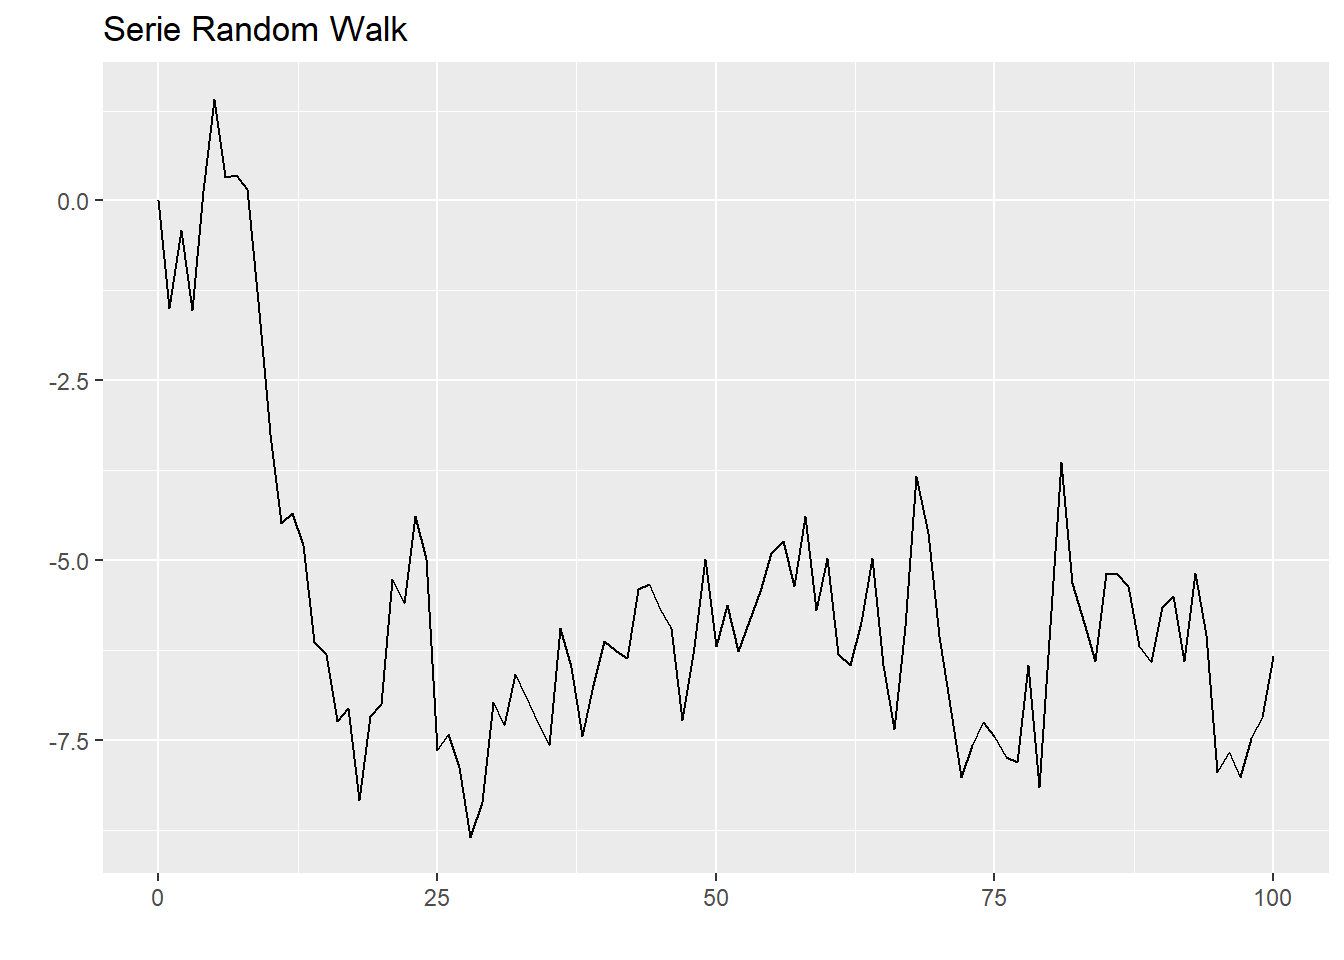
\includegraphics{index_files/figure-latex/unnamed-chunk-4-1.pdf}

\begin{Shaded}
\begin{Highlighting}[]
\NormalTok{white\_noise }\OtherTok{\textless{}{-}} \FunctionTok{arima.sim}\NormalTok{(}\FunctionTok{list}\NormalTok{(}\AttributeTok{order =} \FunctionTok{c}\NormalTok{(}\DecValTok{0}\NormalTok{, }\DecValTok{0}\NormalTok{, }\DecValTok{0}\NormalTok{)), }\AttributeTok{n=}\DecValTok{100}\NormalTok{)}
\NormalTok{random\_walk }\OtherTok{\textless{}{-}} \FunctionTok{cumsum}\NormalTok{(white\_noise)}
\NormalTok{wn\_drift }\OtherTok{\textless{}{-}} \FunctionTok{arima.sim}\NormalTok{(}\FunctionTok{list}\NormalTok{(}\AttributeTok{order =} \FunctionTok{c}\NormalTok{(}\DecValTok{0}\NormalTok{, }\DecValTok{0}\NormalTok{, }\DecValTok{0}\NormalTok{)), }\AttributeTok{n=}\DecValTok{100}\NormalTok{, }\AttributeTok{mean=}\FloatTok{0.4}\NormalTok{)}
\NormalTok{rw\_drift }\OtherTok{\textless{}{-}} \FunctionTok{cumsum}\NormalTok{(wn\_drift)}
\FunctionTok{plot.ts}\NormalTok{(}\FunctionTok{cbind}\NormalTok{(white\_noise, random\_walk, wn\_drift, rw\_drift))}
\end{Highlighting}
\end{Shaded}

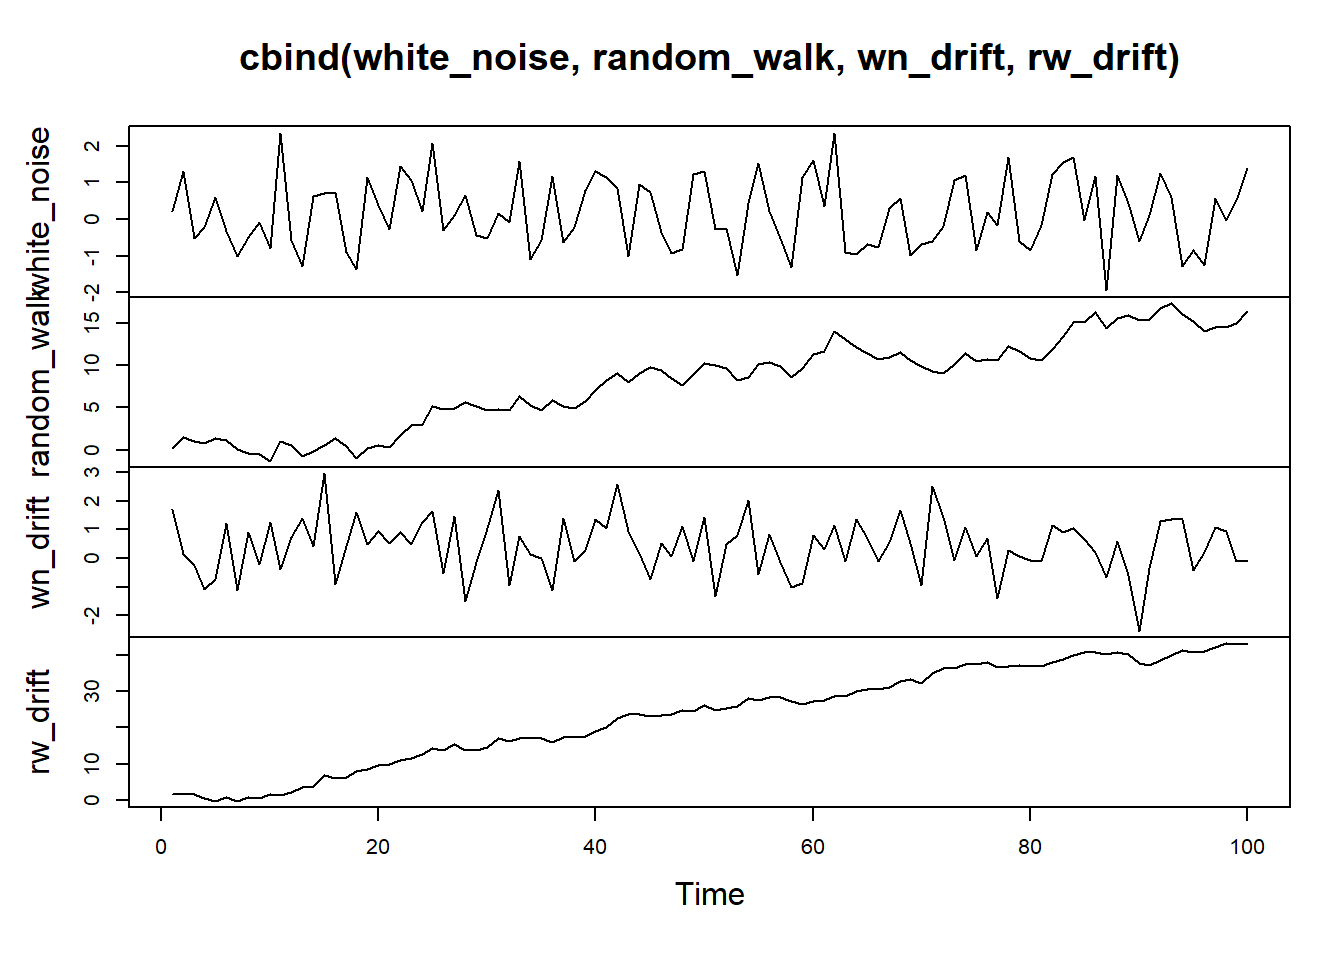
\includegraphics{index_files/figure-latex/unnamed-chunk-5-1.pdf}

\hypertarget{proceso-arma}{%
\section{Proceso ARMA}\label{proceso-arma}}

Simulando un proceso AR(1)

\begin{Shaded}
\begin{Highlighting}[]
\NormalTok{X\_AR1}\OtherTok{\textless{}{-}}\FunctionTok{arima.sim}\NormalTok{(}\FunctionTok{list}\NormalTok{(}\AttributeTok{order=}\FunctionTok{c}\NormalTok{(}\DecValTok{1}\NormalTok{,}\DecValTok{0}\NormalTok{,}\DecValTok{0}\NormalTok{), }\AttributeTok{ar=}\FunctionTok{c}\NormalTok{(}\FloatTok{0.90}\NormalTok{)), }\AttributeTok{n=}\DecValTok{100}\NormalTok{)}
\FunctionTok{autoplot}\NormalTok{(X\_AR1)}
\end{Highlighting}
\end{Shaded}

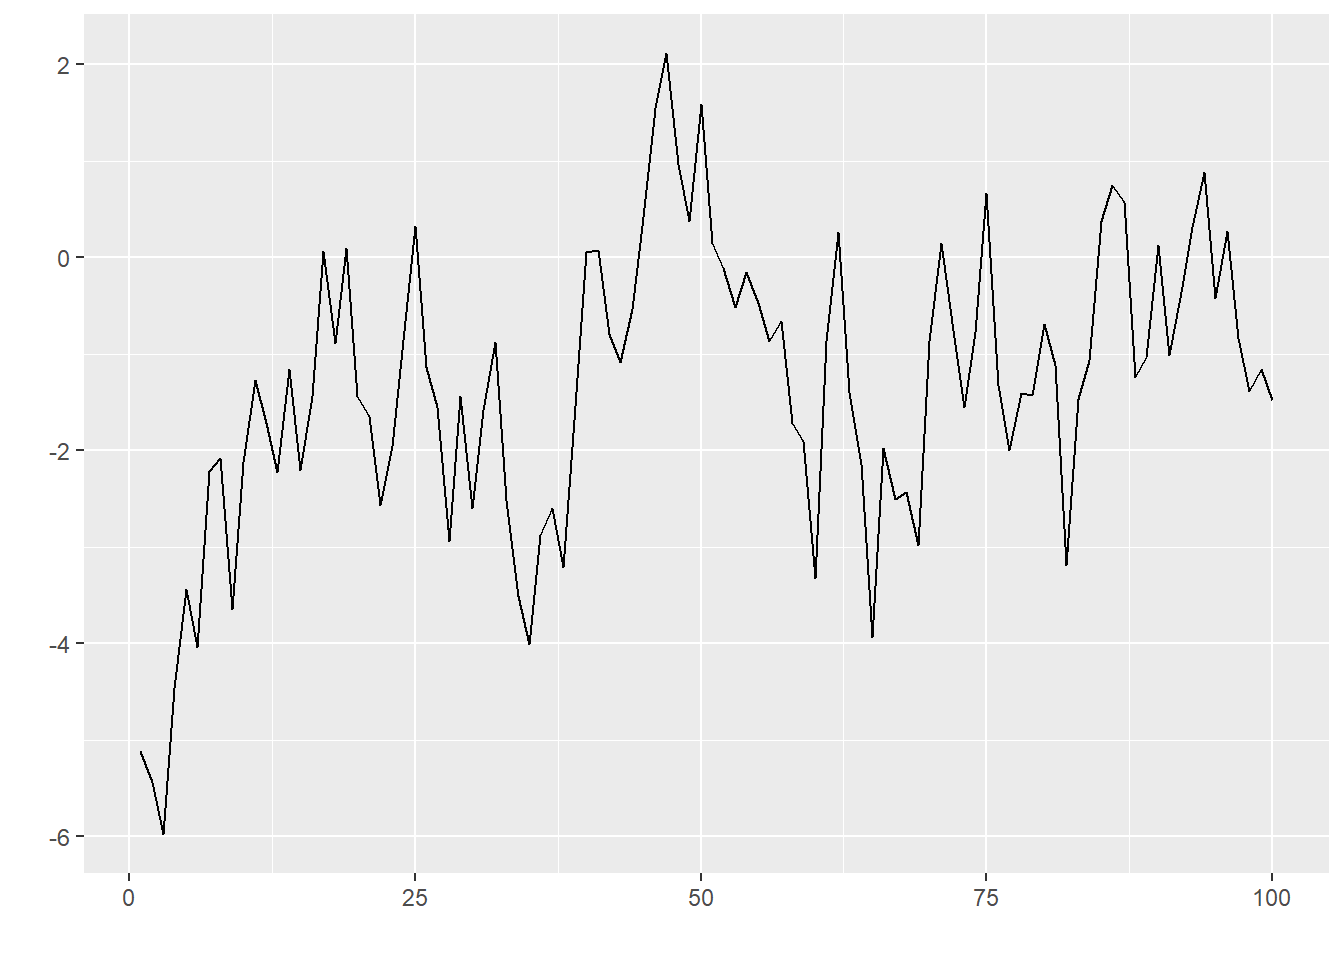
\includegraphics{index_files/figure-latex/unnamed-chunk-6-1.pdf}
Simulando un proceso AR(2)

\begin{Shaded}
\begin{Highlighting}[]
\NormalTok{X\_MA1}\OtherTok{\textless{}{-}}\FunctionTok{arima.sim}\NormalTok{(}\FunctionTok{list}\NormalTok{(}\AttributeTok{order=}\FunctionTok{c}\NormalTok{(}\DecValTok{0}\NormalTok{,}\DecValTok{0}\NormalTok{,}\DecValTok{1}\NormalTok{), }\AttributeTok{ma=}\FunctionTok{c}\NormalTok{(}\SpecialCharTok{{-}}\FloatTok{0.98}\NormalTok{)), }\AttributeTok{n=}\DecValTok{100}\NormalTok{)}\SpecialCharTok{+}\DecValTok{50}
\FunctionTok{autoplot}\NormalTok{(X\_MA1)}
\end{Highlighting}
\end{Shaded}

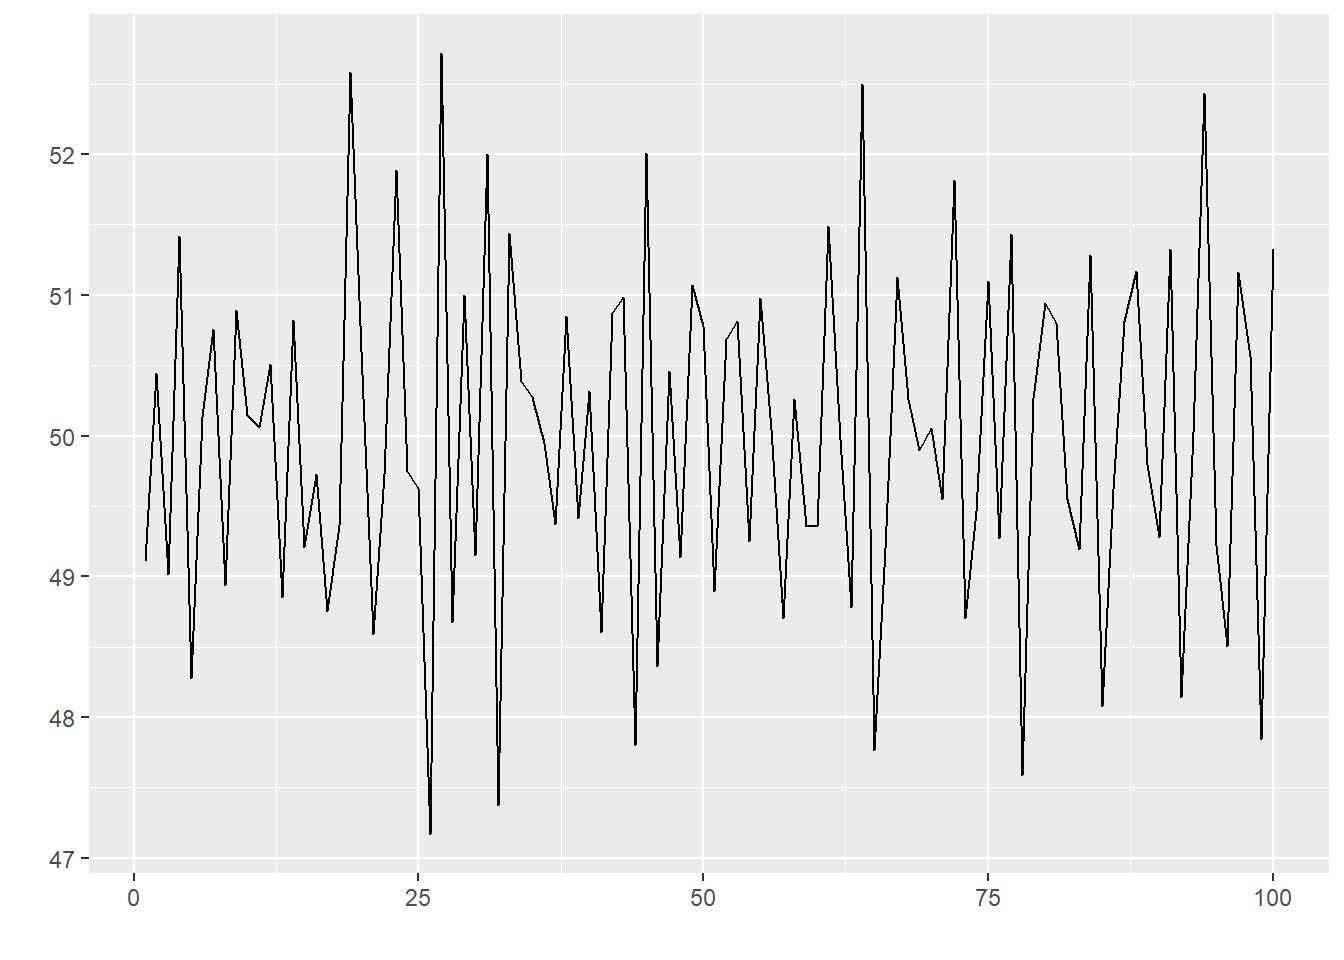
\includegraphics{index_files/figure-latex/unnamed-chunk-7-1.pdf}

Correlación entre el nivel del PIB de Honduras y el de USA

\begin{Shaded}
\begin{Highlighting}[]
\NormalTok{USA}\OtherTok{\textless{}{-}}\FunctionTok{coredata}\NormalTok{(}\FunctionTok{log}\NormalTok{(TRIM}\SpecialCharTok{$}\NormalTok{PIB\_USA[}\StringTok{"2001{-}01{-}01/"}\NormalTok{]))}
\NormalTok{HN}\OtherTok{\textless{}{-}}\FunctionTok{coredata}\NormalTok{(}\FunctionTok{log}\NormalTok{(TRIM}\SpecialCharTok{$}\NormalTok{PIB[}\StringTok{"2001{-}01{-}01/"}\NormalTok{]))}
\FunctionTok{cor}\NormalTok{(USA,HN)}
\end{Highlighting}
\end{Shaded}

\begin{verbatim}
##               PIB
## PIB_USA 0.9775886
\end{verbatim}

Scatter plot

\begin{Shaded}
\begin{Highlighting}[]
\FunctionTok{plot}\NormalTok{(}\FunctionTok{cbind}\NormalTok{(USA, HN))}
\end{Highlighting}
\end{Shaded}

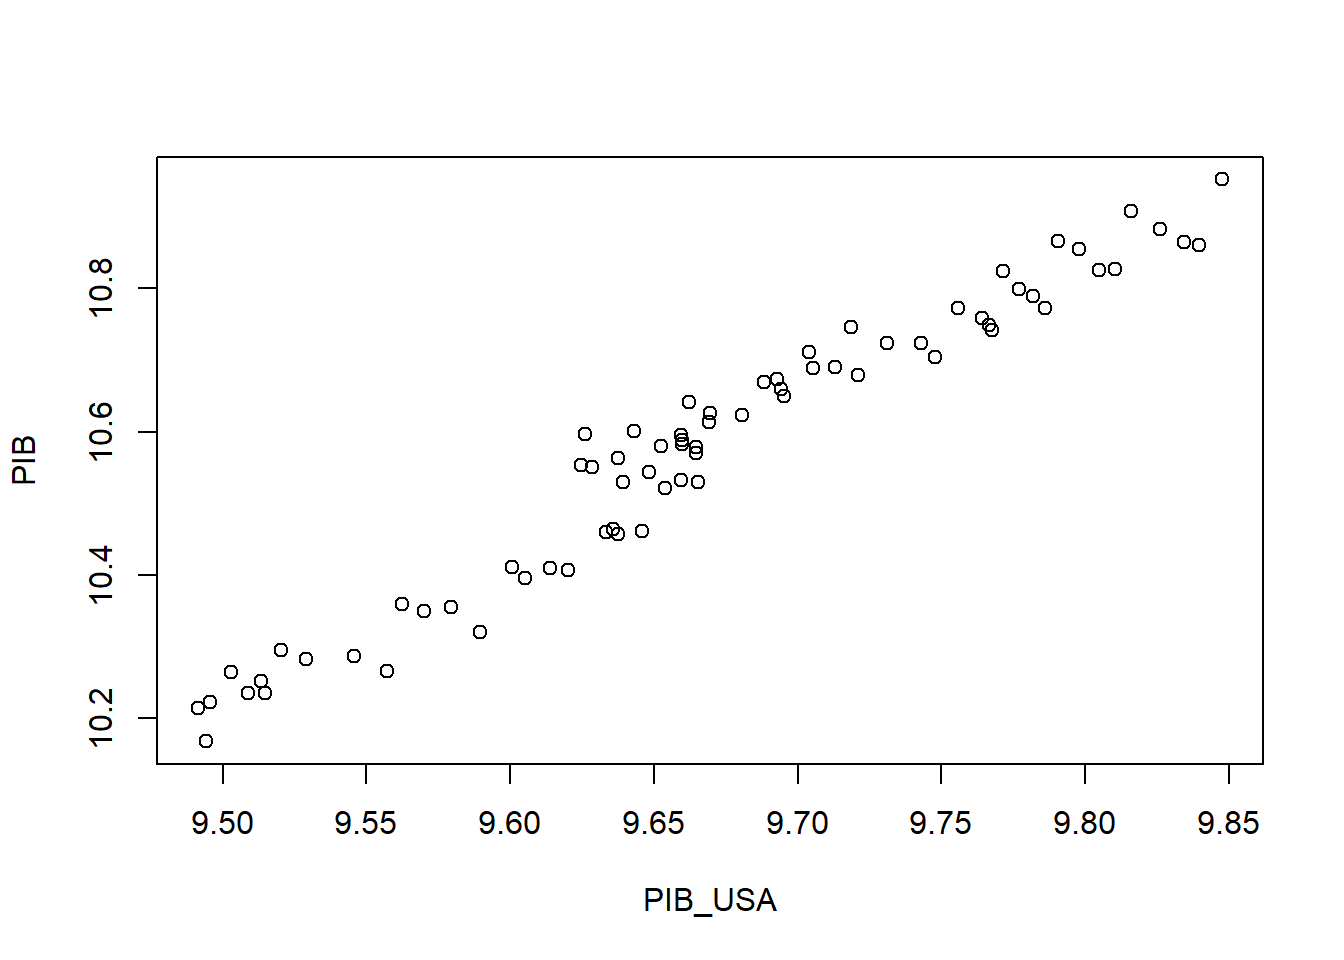
\includegraphics{index_files/figure-latex/unnamed-chunk-9-1.pdf}

Correlación entre el la tasa de crecimiento del PIB de Honduras y el de USA

\begin{Shaded}
\begin{Highlighting}[]
\NormalTok{USA}\OtherTok{\textless{}{-}}\FunctionTok{coredata}\NormalTok{(}\FunctionTok{diff}\NormalTok{(USA, }\AttributeTok{lag=}\DecValTok{4}\NormalTok{))}
\NormalTok{HN}\OtherTok{\textless{}{-}}\FunctionTok{coredata}\NormalTok{(}\FunctionTok{diff}\NormalTok{(HN, }\AttributeTok{lag=}\DecValTok{4}\NormalTok{))}
\FunctionTok{cor}\NormalTok{(USA,HN)}
\end{Highlighting}
\end{Shaded}

\begin{verbatim}
##               PIB
## PIB_USA 0.5405966
\end{verbatim}

Scatter plot

\begin{Shaded}
\begin{Highlighting}[]
\FunctionTok{plot}\NormalTok{(USA, HN)}
\end{Highlighting}
\end{Shaded}

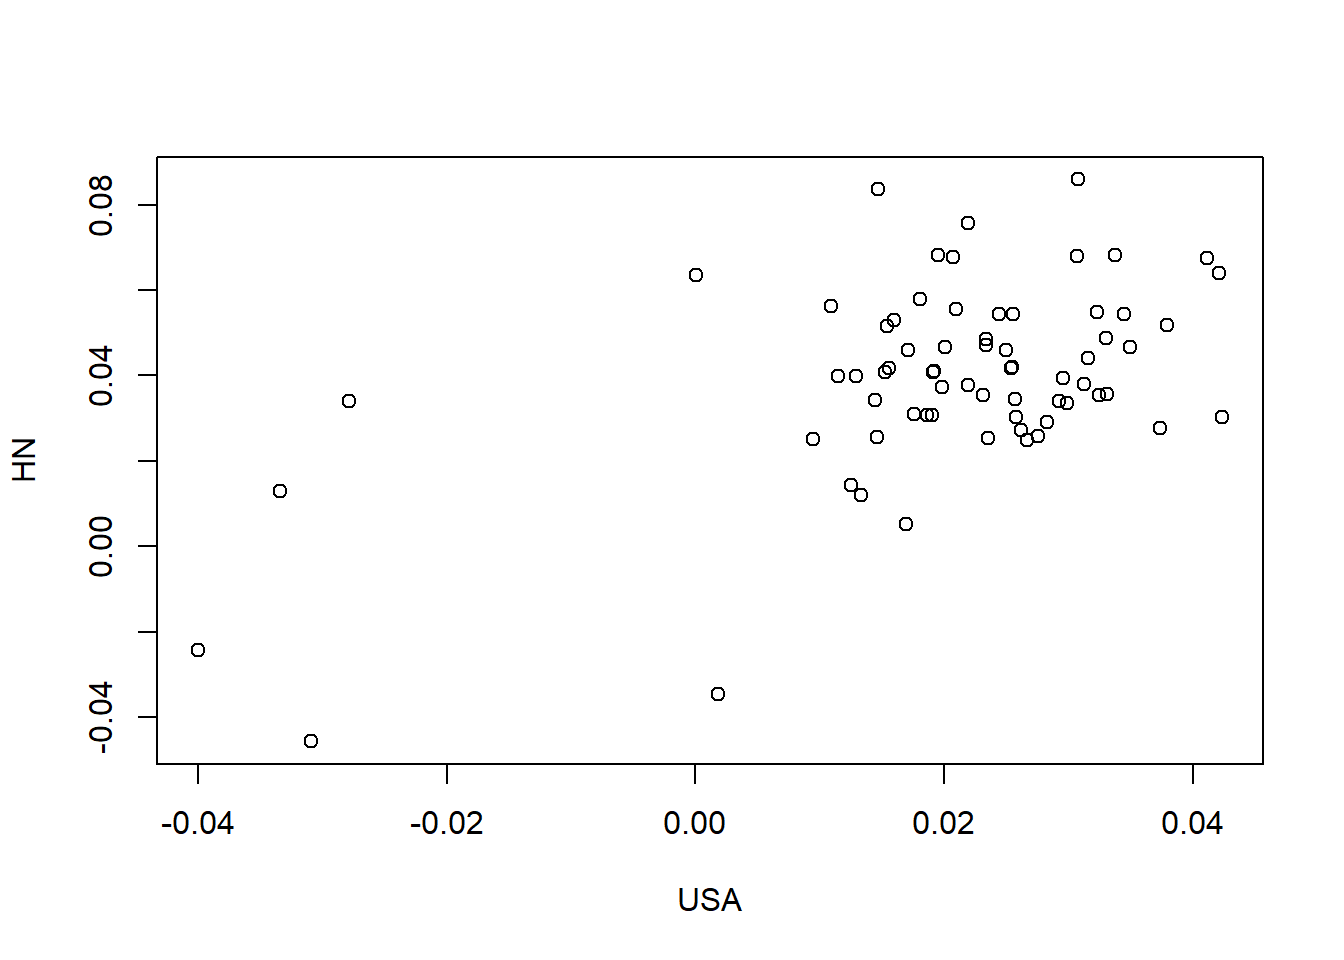
\includegraphics{index_files/figure-latex/unnamed-chunk-11-1.pdf}

Función de autocorrelación del PIB de Honduras

\begin{Shaded}
\begin{Highlighting}[]
\NormalTok{PIB}\OtherTok{\textless{}{-}}\FunctionTok{as.ts}\NormalTok{(HN)}
\FunctionTok{acf}\NormalTok{(PIB, }\AttributeTok{lag.max =} \DecValTok{24}\NormalTok{, }\AttributeTok{plot=}\ConstantTok{TRUE}\NormalTok{)}
\end{Highlighting}
\end{Shaded}

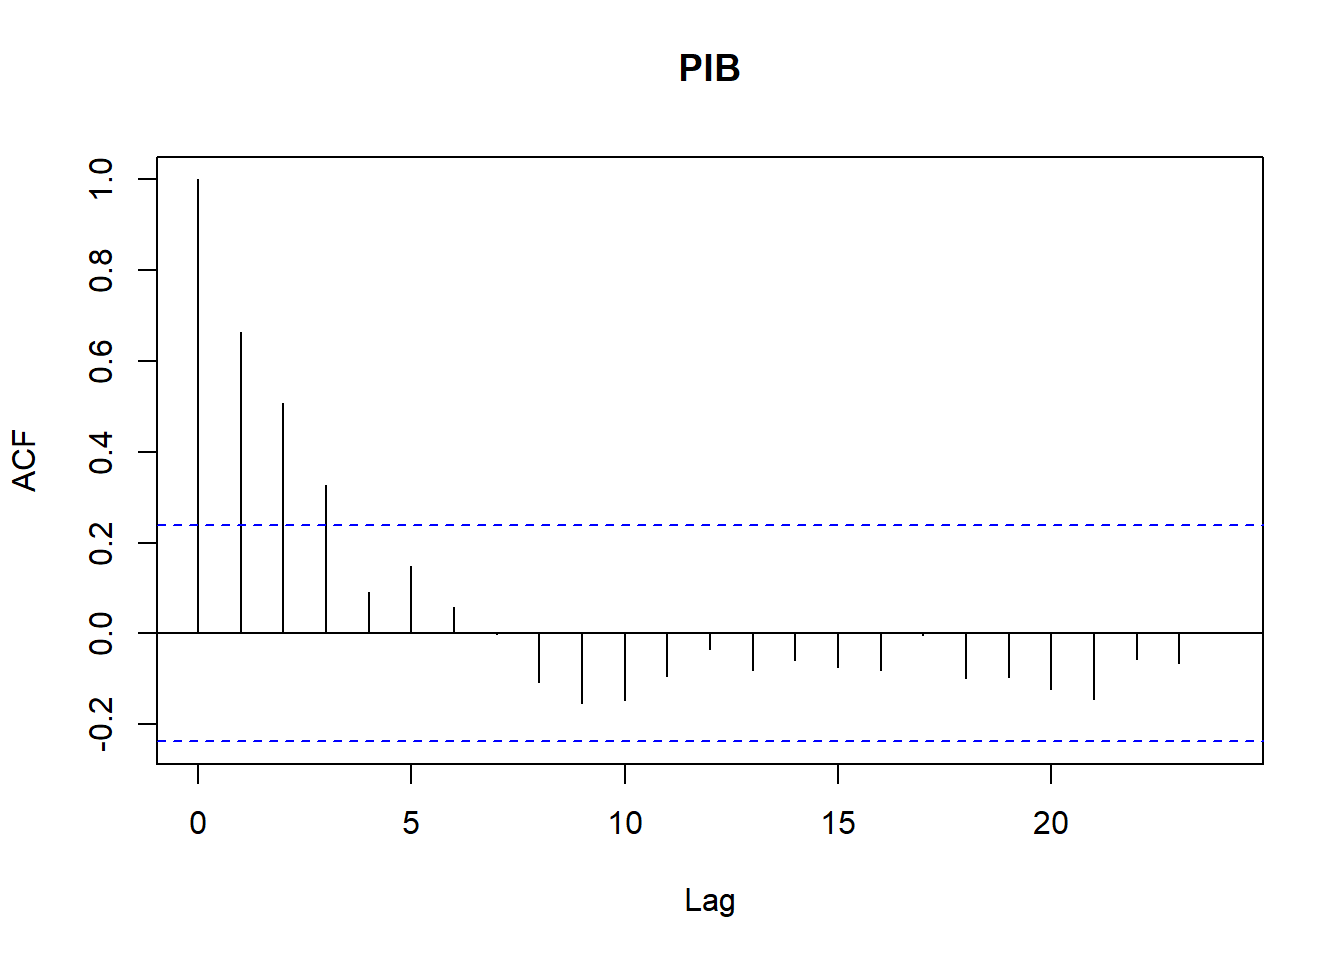
\includegraphics{index_files/figure-latex/unnamed-chunk-12-1.pdf}

Función de autocorrelación parcial del PIB de Honduras

\begin{Shaded}
\begin{Highlighting}[]
\NormalTok{PIB}\OtherTok{\textless{}{-}}\FunctionTok{as.ts}\NormalTok{(HN)}
\FunctionTok{pacf}\NormalTok{(PIB, }\AttributeTok{lag.max =} \DecValTok{24}\NormalTok{, }\AttributeTok{plot=}\ConstantTok{TRUE}\NormalTok{)}
\end{Highlighting}
\end{Shaded}

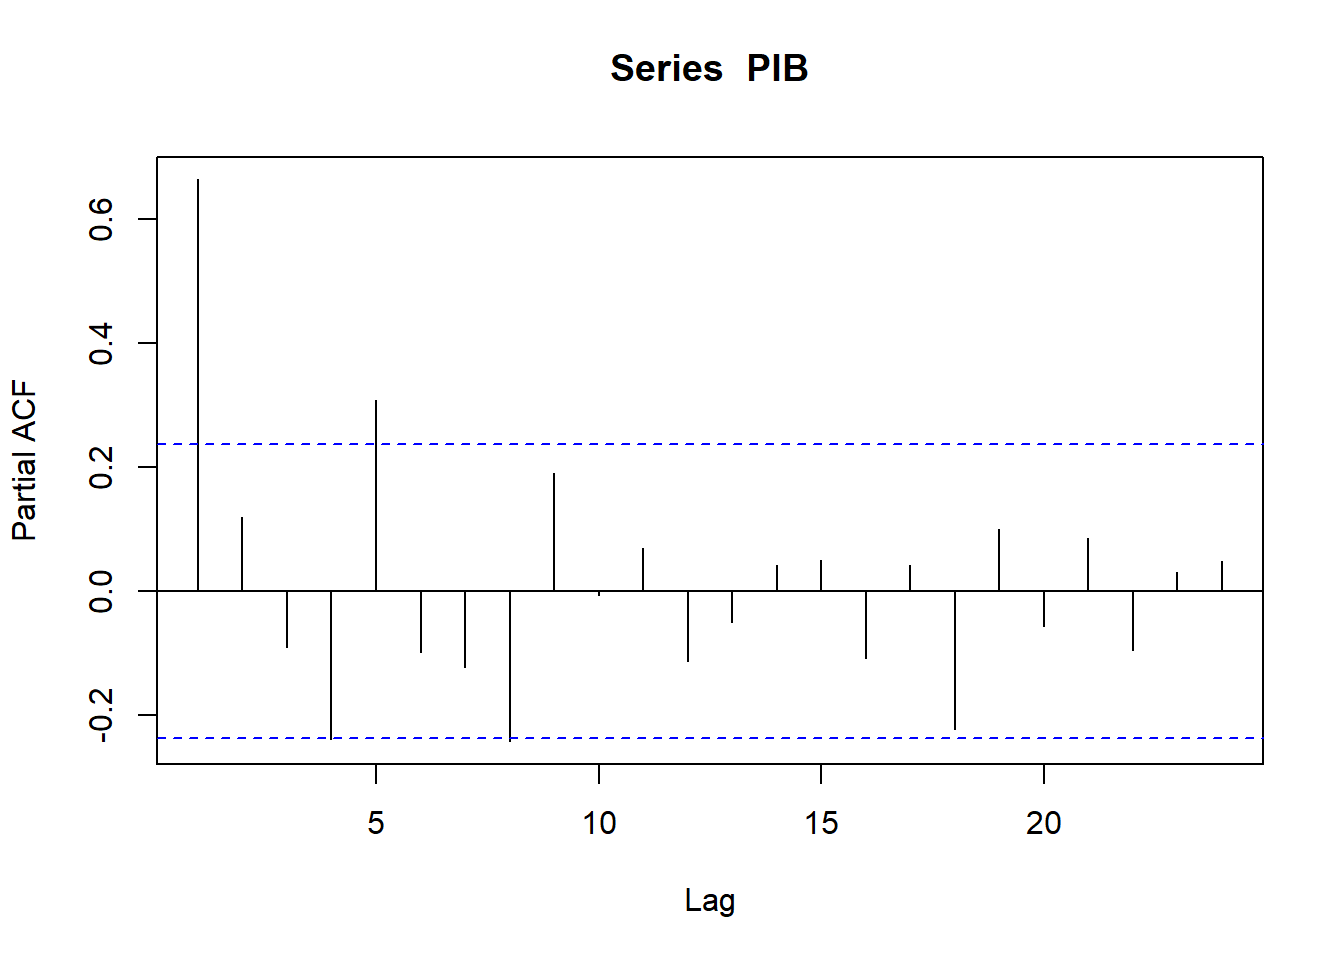
\includegraphics{index_files/figure-latex/unnamed-chunk-13-1.pdf}

Función de autocorrelación de un proceso ruído blanco

\begin{Shaded}
\begin{Highlighting}[]
\FunctionTok{acf}\NormalTok{(X\_WN, }\AttributeTok{lag.max =} \DecValTok{24}\NormalTok{, }\AttributeTok{plot=}\ConstantTok{TRUE}\NormalTok{)}
\end{Highlighting}
\end{Shaded}

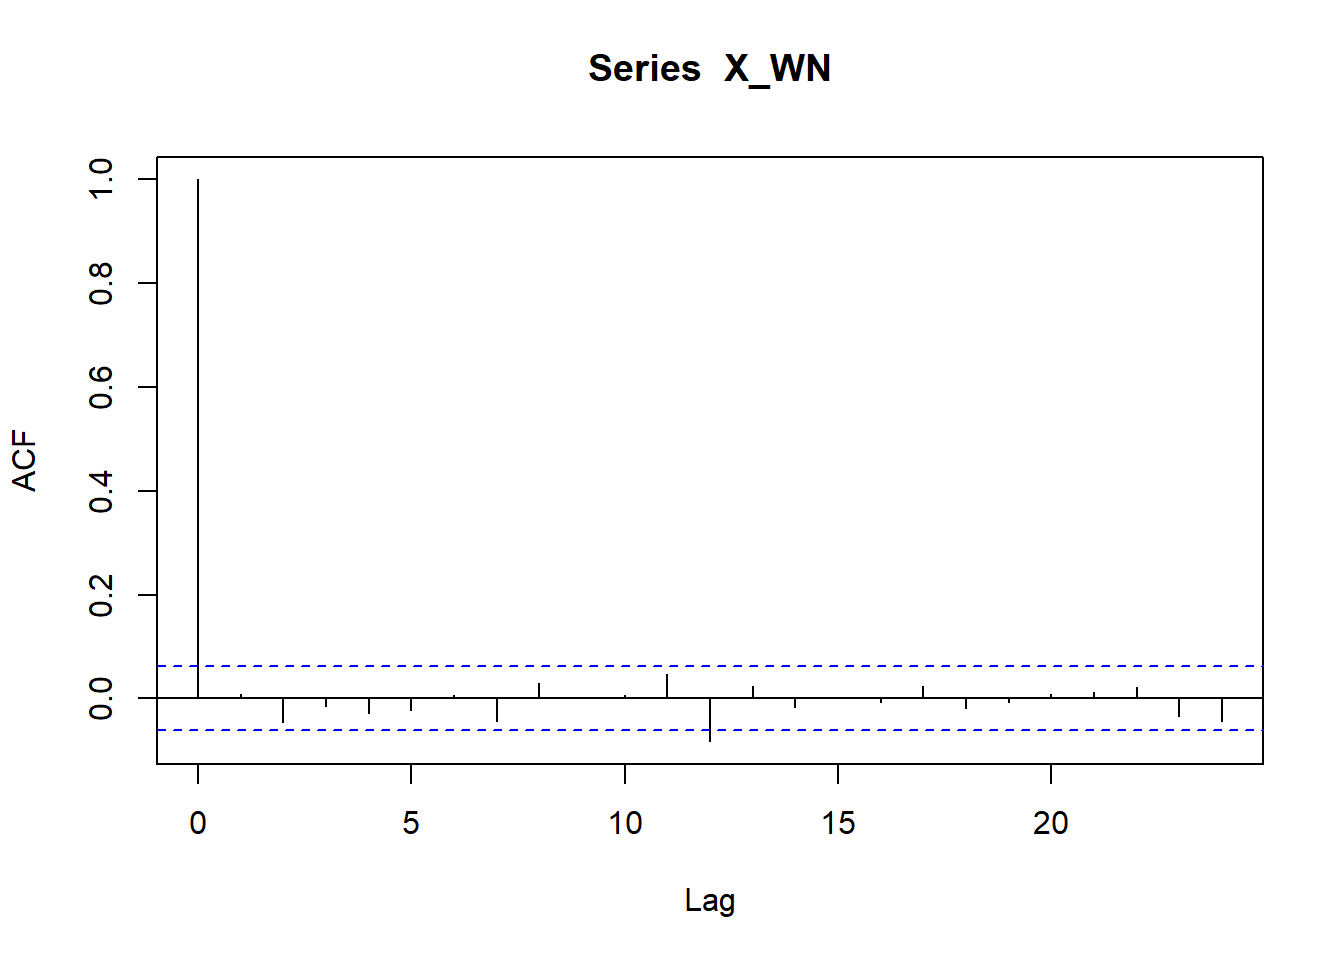
\includegraphics{index_files/figure-latex/unnamed-chunk-14-1.pdf}

Función de autocorrelación parcial de un proceso ruído blanco

\begin{Shaded}
\begin{Highlighting}[]
\FunctionTok{pacf}\NormalTok{(X\_WN, }\AttributeTok{lag.max =} \DecValTok{24}\NormalTok{, }\AttributeTok{plot=}\ConstantTok{TRUE}\NormalTok{)}
\end{Highlighting}
\end{Shaded}

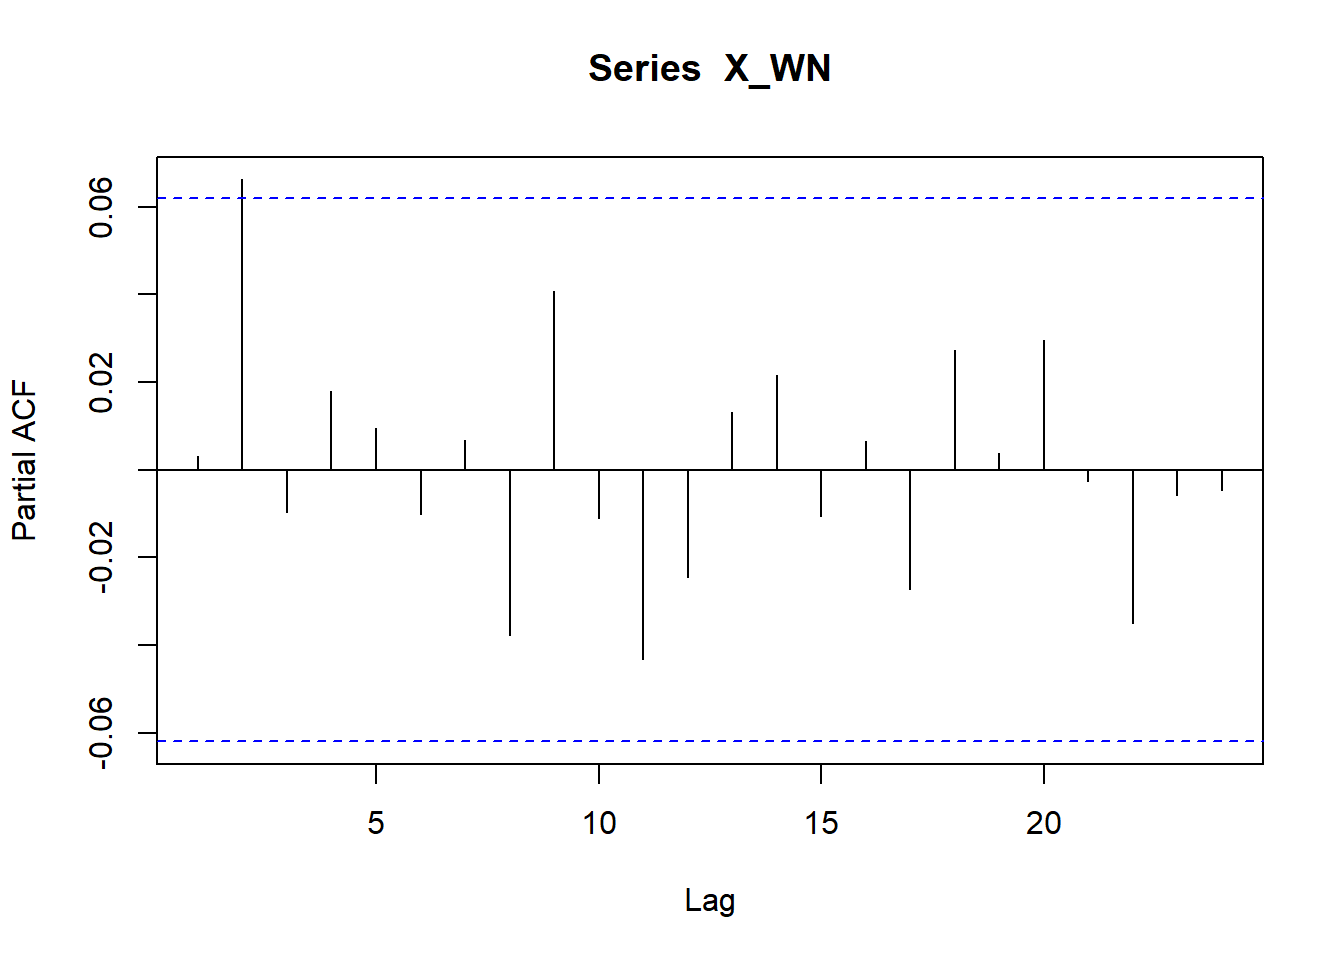
\includegraphics{index_files/figure-latex/unnamed-chunk-15-1.pdf}

Función de autocorrelación de un proceso RW

\begin{Shaded}
\begin{Highlighting}[]
\FunctionTok{acf}\NormalTok{(X\_RW, }\AttributeTok{lag.max =} \DecValTok{24}\NormalTok{, }\AttributeTok{plot=}\ConstantTok{TRUE}\NormalTok{)}
\end{Highlighting}
\end{Shaded}

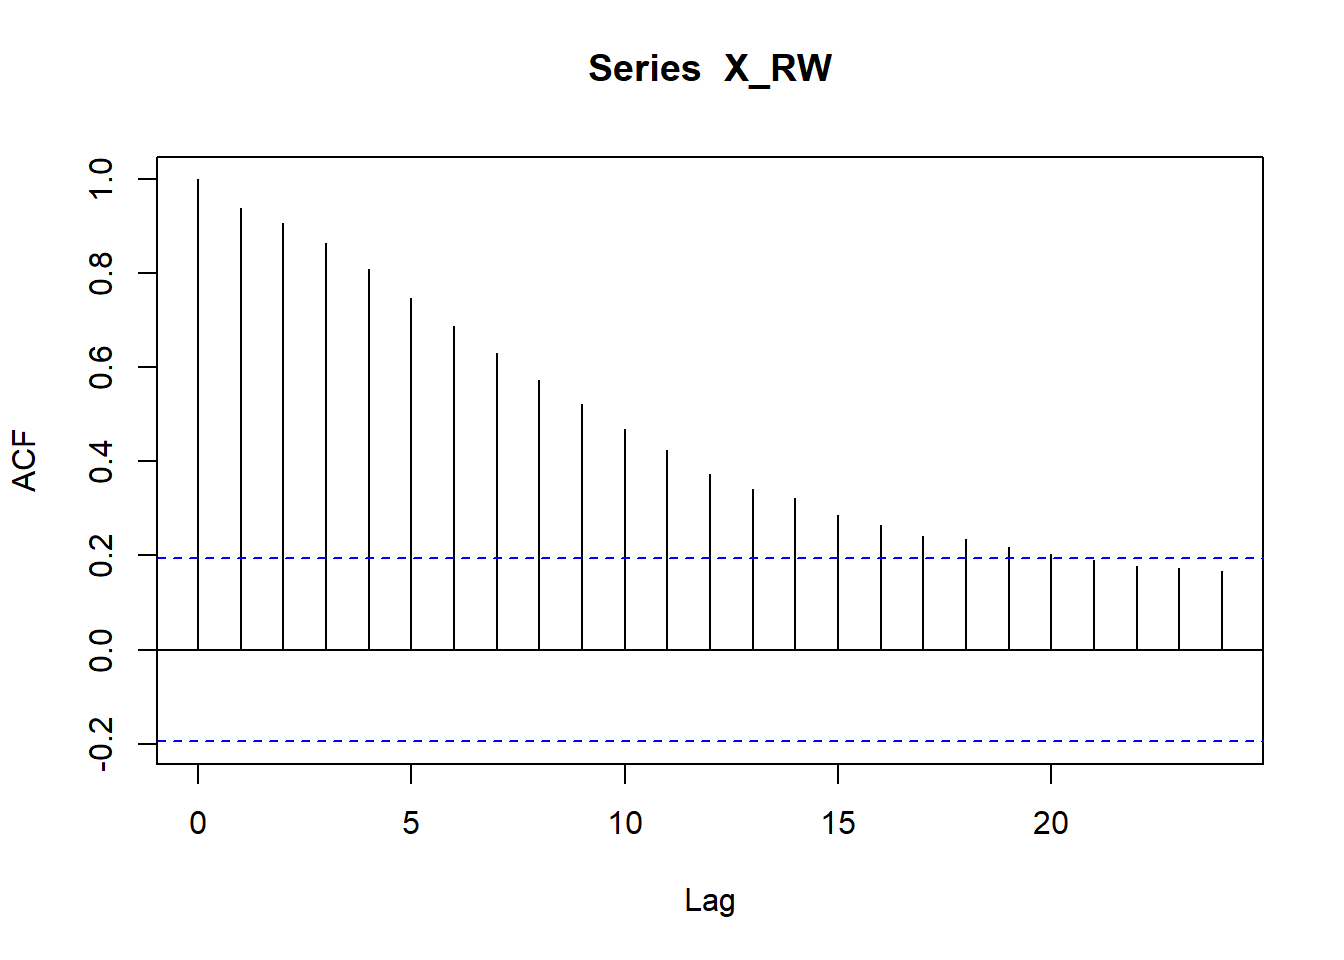
\includegraphics{index_files/figure-latex/unnamed-chunk-16-1.pdf}

Función de autocorrelación parcial de un proceso RW

\begin{Shaded}
\begin{Highlighting}[]
\FunctionTok{pacf}\NormalTok{(X\_RW, }\AttributeTok{lag.max =} \DecValTok{24}\NormalTok{, }\AttributeTok{plot=}\ConstantTok{TRUE}\NormalTok{)}
\end{Highlighting}
\end{Shaded}

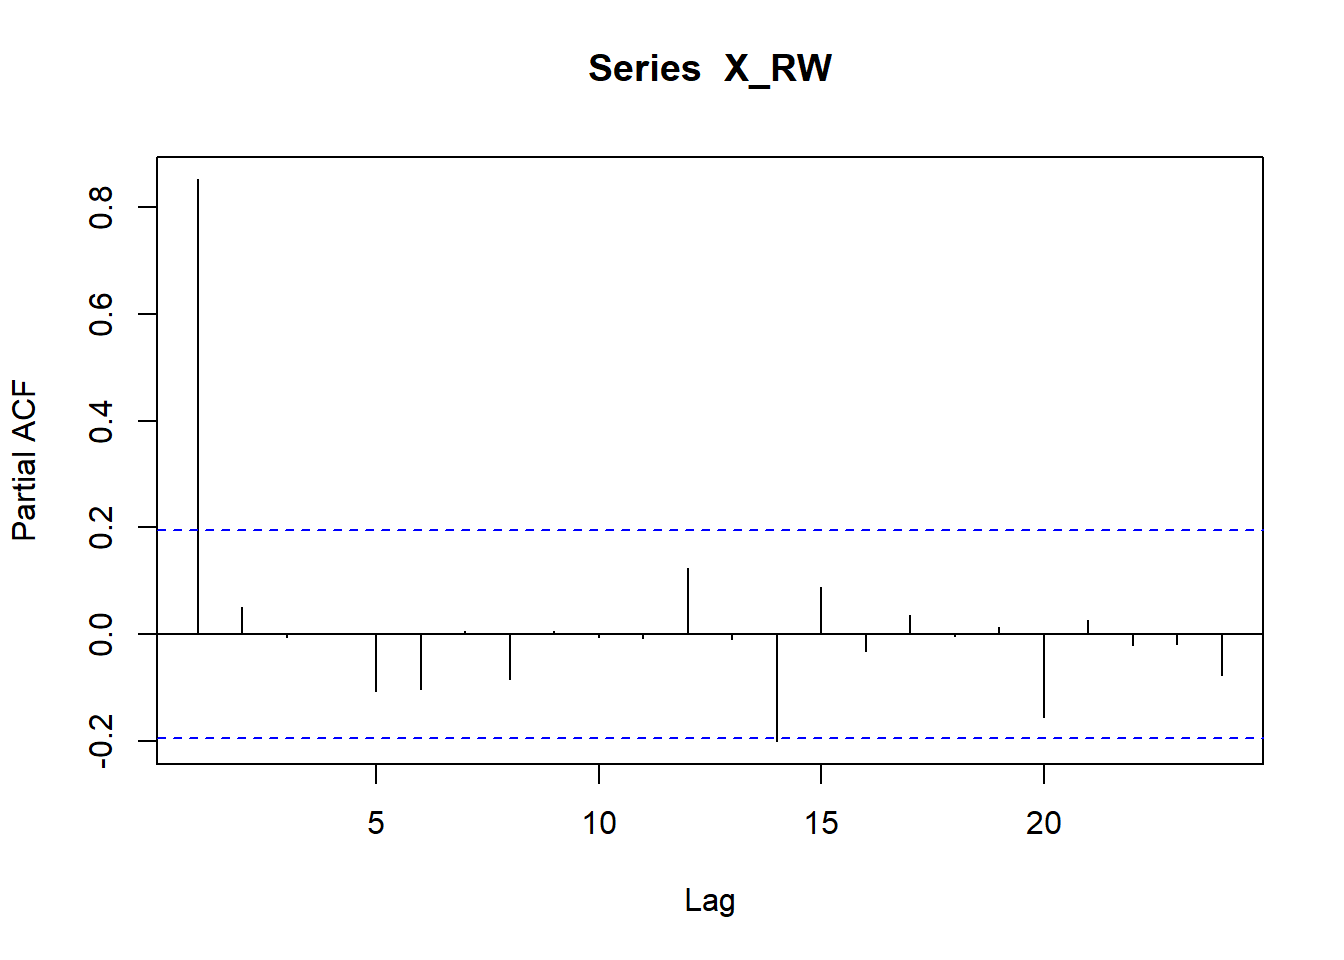
\includegraphics{index_files/figure-latex/unnamed-chunk-17-1.pdf}

Función de autocorrelación de un proceso AR(1)

\begin{Shaded}
\begin{Highlighting}[]
\FunctionTok{acf}\NormalTok{(X\_AR1, }\AttributeTok{lag.max =} \DecValTok{24}\NormalTok{, }\AttributeTok{plot=}\ConstantTok{TRUE}\NormalTok{)}
\end{Highlighting}
\end{Shaded}

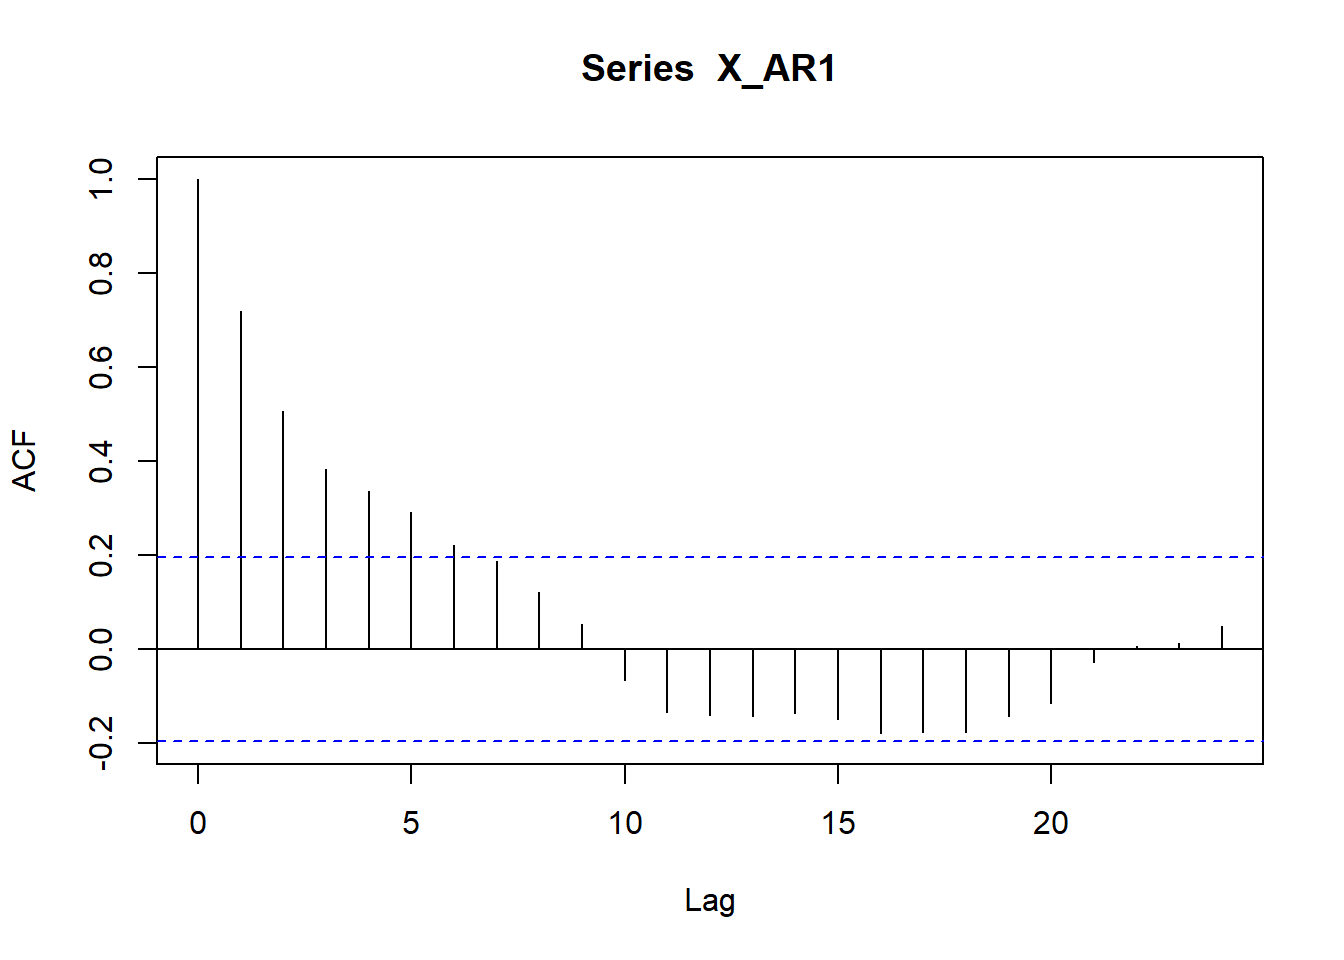
\includegraphics{index_files/figure-latex/unnamed-chunk-18-1.pdf}

Función de autocorrelación parcial de un proceso AR(1)

\begin{Shaded}
\begin{Highlighting}[]
\FunctionTok{pacf}\NormalTok{(X\_AR1, }\AttributeTok{lag.max =} \DecValTok{24}\NormalTok{, }\AttributeTok{plot=}\ConstantTok{TRUE}\NormalTok{)}
\end{Highlighting}
\end{Shaded}

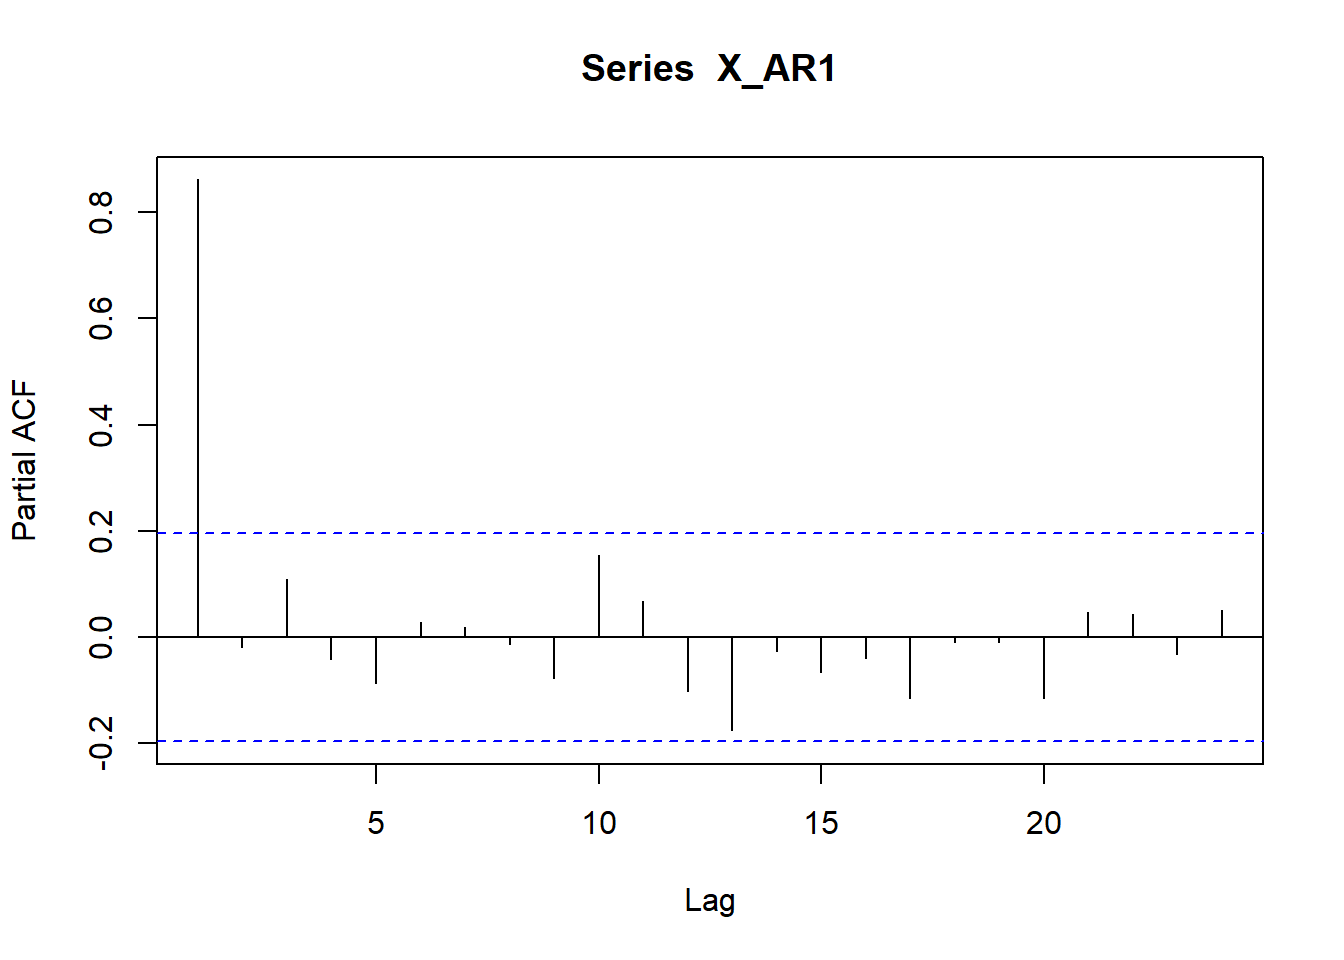
\includegraphics{index_files/figure-latex/unnamed-chunk-19-1.pdf}

Función de autocorrelación de un proceso MA(1)

\begin{Shaded}
\begin{Highlighting}[]
\FunctionTok{acf}\NormalTok{(X\_MA1, }\AttributeTok{lag.max =} \DecValTok{24}\NormalTok{, }\AttributeTok{plot=}\ConstantTok{TRUE}\NormalTok{)}
\end{Highlighting}
\end{Shaded}

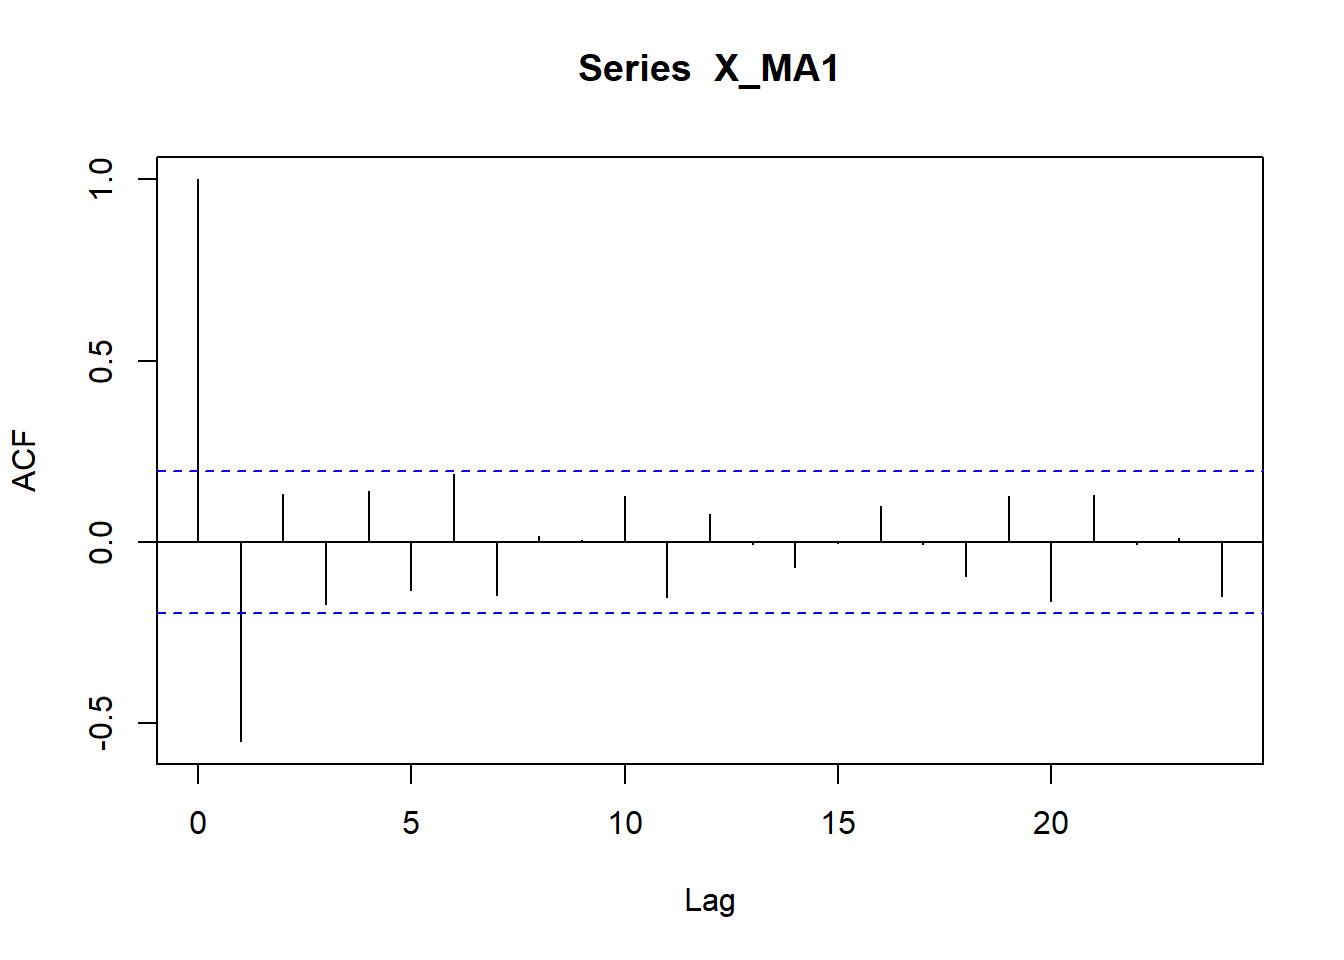
\includegraphics{index_files/figure-latex/unnamed-chunk-20-1.pdf}

Función de autocorrelación parcial de un proceso MA(1)

\begin{Shaded}
\begin{Highlighting}[]
\FunctionTok{pacf}\NormalTok{(X\_MA1, }\AttributeTok{lag.max =} \DecValTok{24}\NormalTok{, }\AttributeTok{plot=}\ConstantTok{TRUE}\NormalTok{)}
\end{Highlighting}
\end{Shaded}

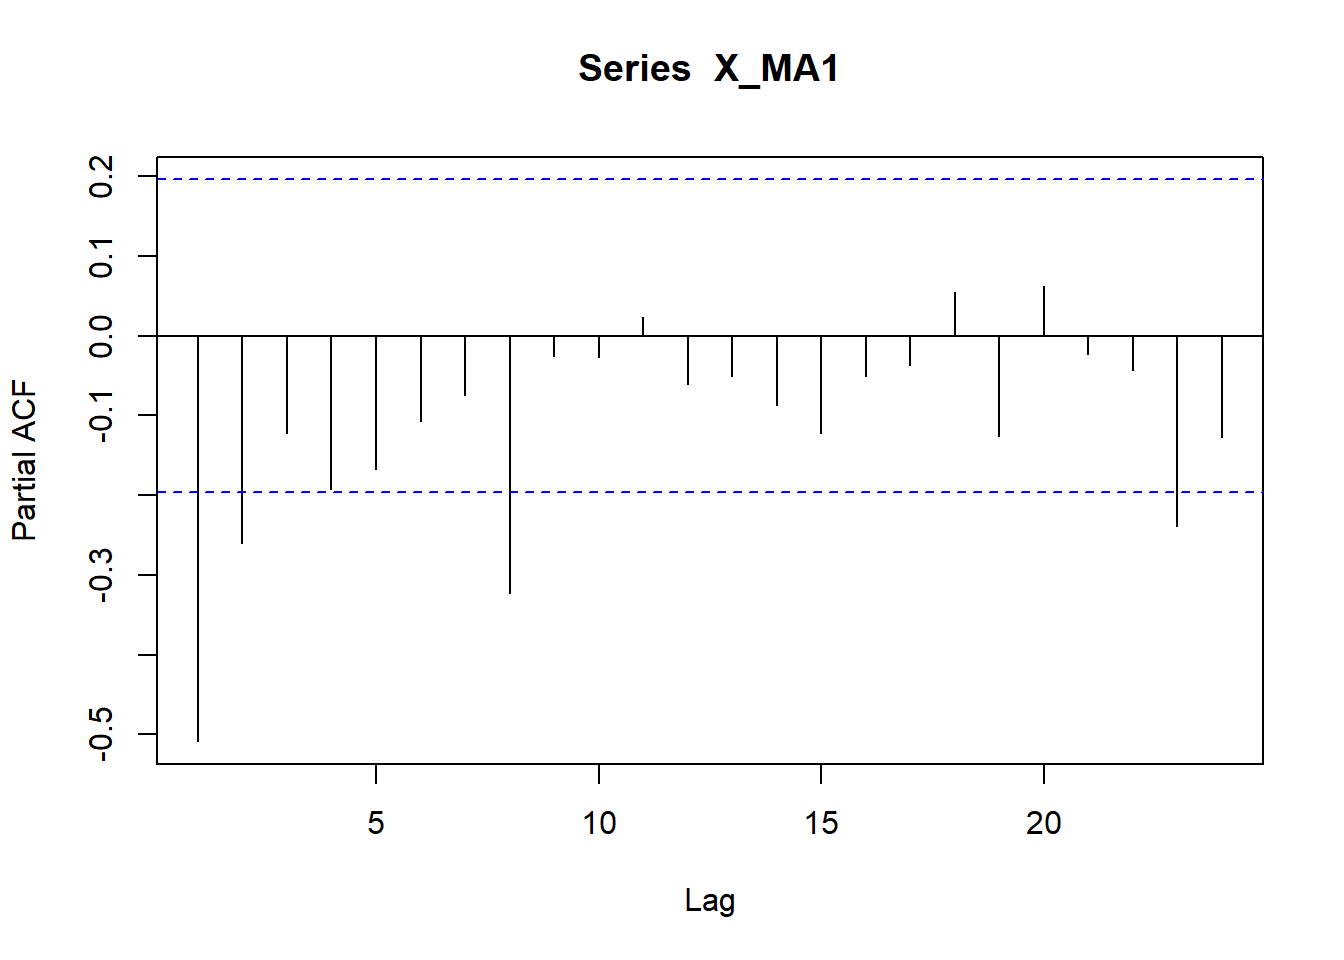
\includegraphics{index_files/figure-latex/unnamed-chunk-21-1.pdf}

\hypertarget{simulaciuxf3n-de-procesos}{%
\section{Simulación de procesos}\label{simulaciuxf3n-de-procesos}}

\#\#\#Estimación de un procesos SARIMA(1,0,1,1,1,1)

\begin{Shaded}
\begin{Highlighting}[]
\NormalTok{model    }\OtherTok{\textless{}{-}} \FunctionTok{Arima}\NormalTok{(}\FunctionTok{ts}\NormalTok{(}\FunctionTok{rnorm}\NormalTok{(}\DecValTok{100}\NormalTok{),}\AttributeTok{freq=}\DecValTok{4}\NormalTok{), }\AttributeTok{order=}\FunctionTok{c}\NormalTok{(}\DecValTok{1}\NormalTok{,}\DecValTok{0}\NormalTok{,}\DecValTok{1}\NormalTok{), }\AttributeTok{seasonal=}\FunctionTok{c}\NormalTok{(}\DecValTok{1}\NormalTok{,}\DecValTok{1}\NormalTok{,}\DecValTok{1}\NormalTok{),}
            \AttributeTok{fixed=}\FunctionTok{c}\NormalTok{(}\AttributeTok{phi=}\FloatTok{0.0}\NormalTok{, }\AttributeTok{theta=}\SpecialCharTok{{-}}\FloatTok{0.0}\NormalTok{, }\AttributeTok{Phi=}\FloatTok{0.0}\NormalTok{, }\AttributeTok{Theta=}\SpecialCharTok{{-}}\FloatTok{0.0}\NormalTok{))}
\NormalTok{X\_SARIMA}\OtherTok{\textless{}{-}} \FunctionTok{simulate}\NormalTok{(model, }\AttributeTok{nsim=}\DecValTok{200}\NormalTok{)}
\FunctionTok{plot}\NormalTok{(X\_SARIMA)}
\end{Highlighting}
\end{Shaded}

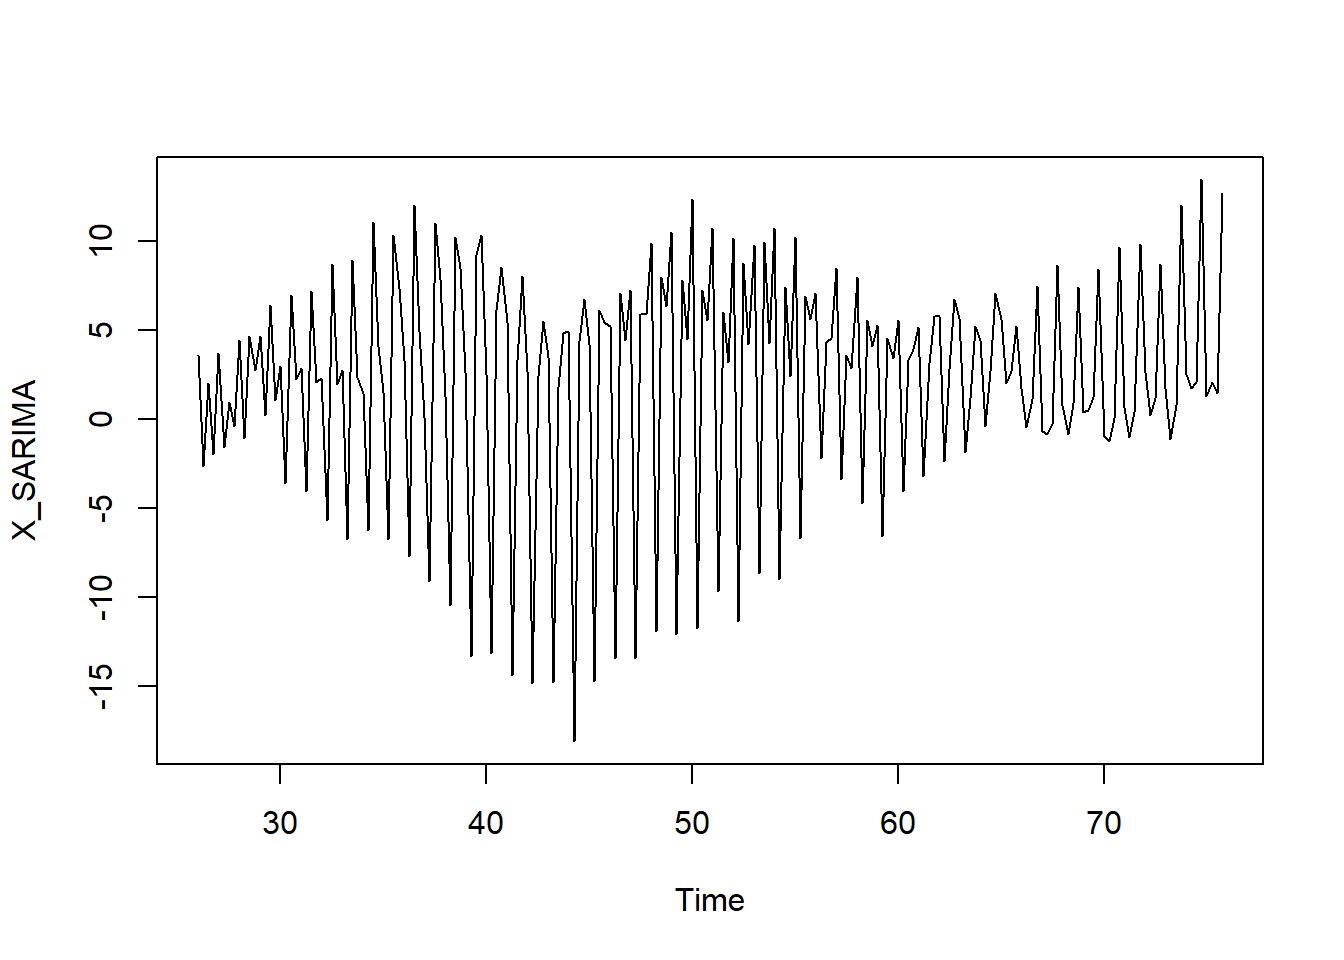
\includegraphics{index_files/figure-latex/unnamed-chunk-22-1.pdf}

\hypertarget{estimaciuxf3n-de-un-proceso-arima}{%
\subsection{Estimación de un proceso ARIMA}\label{estimaciuxf3n-de-un-proceso-arima}}

\begin{Shaded}
\begin{Highlighting}[]
\NormalTok{x}\OtherTok{\textless{}{-}}\FunctionTok{arima.sim}\NormalTok{(}\FunctionTok{list}\NormalTok{(}\AttributeTok{order=}\FunctionTok{c}\NormalTok{(}\DecValTok{0}\NormalTok{,}\DecValTok{0}\NormalTok{,}\DecValTok{2}\NormalTok{), }\AttributeTok{ma=}\FunctionTok{c}\NormalTok{(}\FloatTok{1.5}\NormalTok{,}\SpecialCharTok{{-}}\FloatTok{0.75}\NormalTok{)), }\AttributeTok{n=}\DecValTok{100}\NormalTok{)}\SpecialCharTok{+}\DecValTok{50}
\NormalTok{x\_fit}\OtherTok{\textless{}{-}}\FunctionTok{sarima}\NormalTok{(x, }\AttributeTok{p=}\DecValTok{2}\NormalTok{, }\AttributeTok{d=}\DecValTok{0}\NormalTok{, }\AttributeTok{q=}\DecValTok{0}\NormalTok{)}
\end{Highlighting}
\end{Shaded}

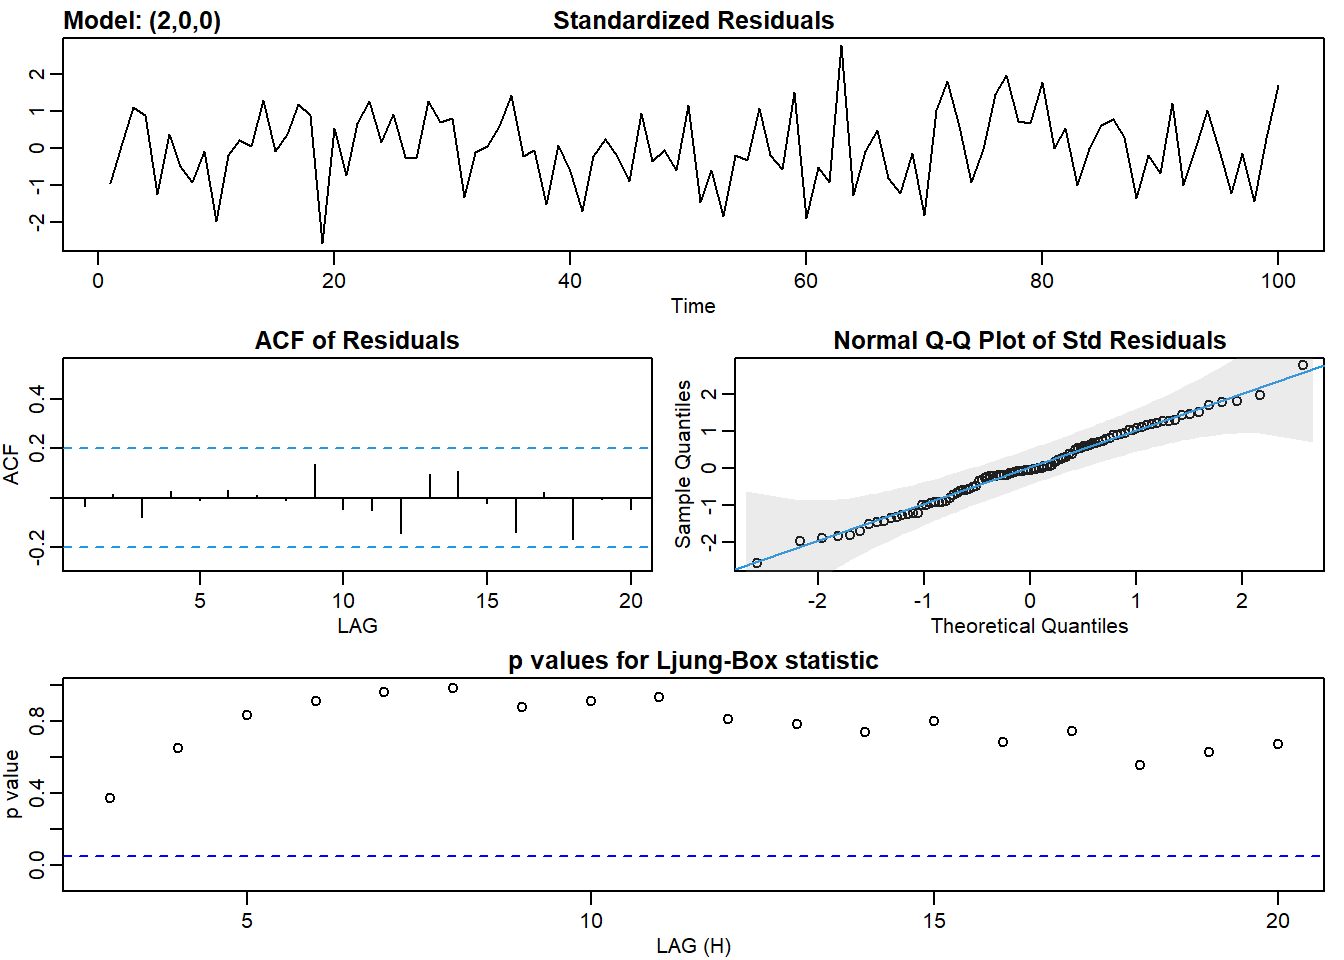
\includegraphics{index_files/figure-latex/unnamed-chunk-23-1.pdf}

\begin{Shaded}
\begin{Highlighting}[]
\NormalTok{x\_fit}\SpecialCharTok{$}\NormalTok{ttable}
\end{Highlighting}
\end{Shaded}

\hypertarget{pronuxf3sticos}{%
\chapter{Pronósticos}\label{pronuxf3sticos}}

\hypertarget{modelos-introductorios}{%
\section{Modelos introductorios}\label{modelos-introductorios}}

Pronósticos Naive del IMAE de Honduras vs data observada

\begin{Shaded}
\begin{Highlighting}[]
\NormalTok{imae}\OtherTok{\textless{}{-}}\FunctionTok{log}\NormalTok{(MES}\SpecialCharTok{$}\NormalTok{IMAE[}\StringTok{"2001{-}01{-}01/2010{-}12{-}01"}\NormalTok{])}
\NormalTok{IMAE\_NAIVE}\OtherTok{\textless{}{-}}\FunctionTok{naive}\NormalTok{(imae)}
\NormalTok{imaef}\OtherTok{\textless{}{-}}\FunctionTok{ts}\NormalTok{(}\FunctionTok{fitted}\NormalTok{(IMAE\_NAIVE), }\AttributeTok{frequency=}\DecValTok{12}\NormalTok{, }\AttributeTok{start=}\FunctionTok{c}\NormalTok{(}\DecValTok{2001}\SpecialCharTok{/}\DecValTok{01}\SpecialCharTok{/}\DecValTok{01}\NormalTok{))}
\NormalTok{imaef}\OtherTok{\textless{}{-}}\FunctionTok{as.xts}\NormalTok{(imaef)}
\FunctionTok{autoplot}\NormalTok{(}\FunctionTok{ts}\NormalTok{(}\FunctionTok{cbind}\NormalTok{(imae, imaef), }\AttributeTok{start =} \FunctionTok{c}\NormalTok{(}\DecValTok{2001}\SpecialCharTok{/}\DecValTok{01}\SpecialCharTok{/}\DecValTok{01}\NormalTok{), }\AttributeTok{frequency =} \DecValTok{12}\NormalTok{ ),}
         \AttributeTok{facets =} \ConstantTok{FALSE}\NormalTok{)}\SpecialCharTok{+}\FunctionTok{xlab}\NormalTok{(}\StringTok{"Years"}\NormalTok{)}
\end{Highlighting}
\end{Shaded}

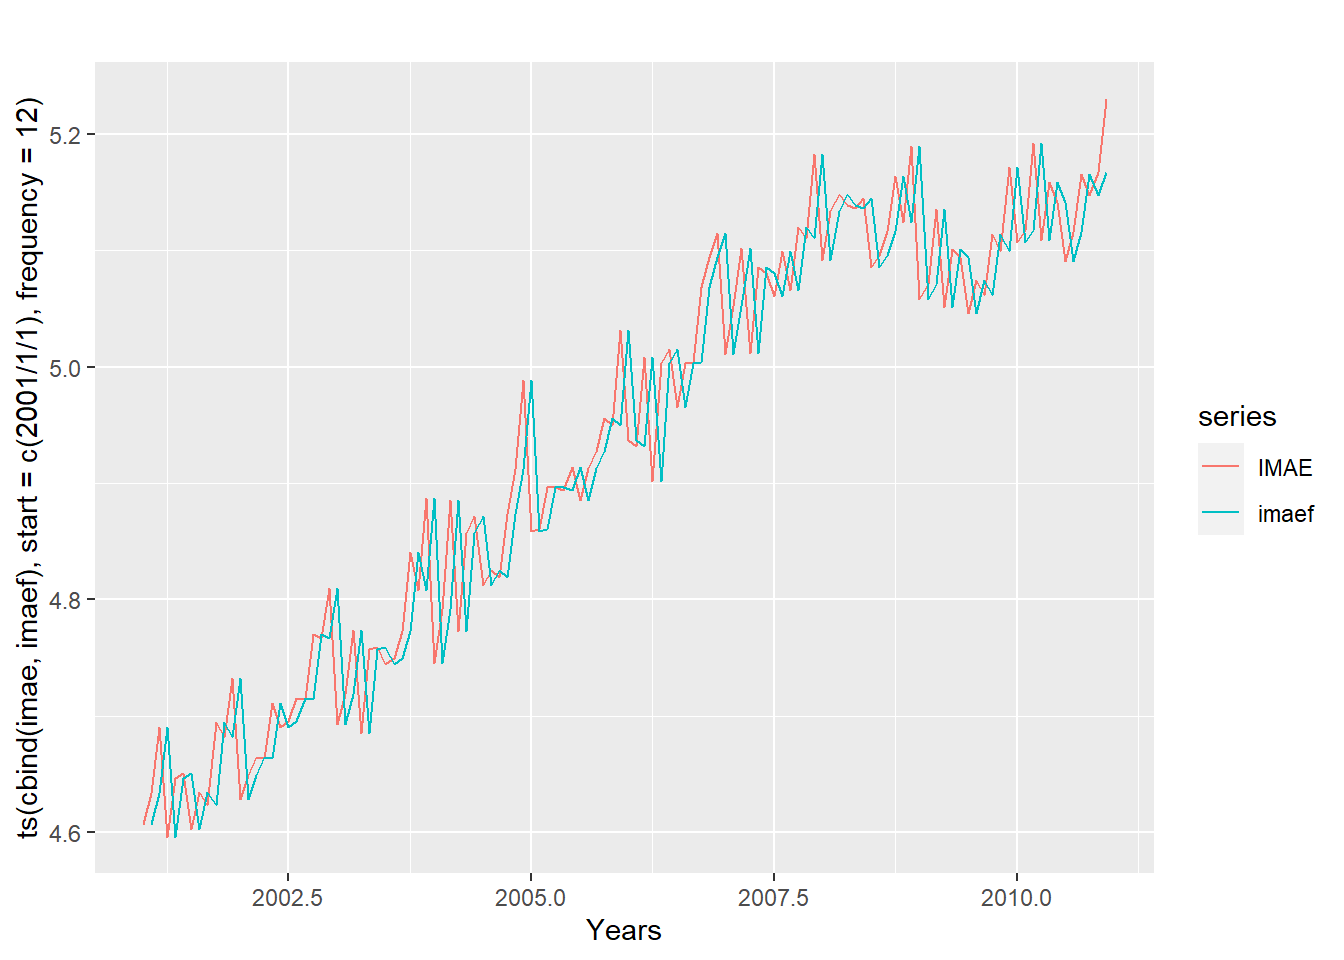
\includegraphics{index_files/figure-latex/unnamed-chunk-24-1.pdf}

Pronósticos del IMAE de Honduras 24 meses en adelante a partir de un proceso SARIMA(1,1,1)

\begin{Shaded}
\begin{Highlighting}[]
\NormalTok{imae}\OtherTok{\textless{}{-}}\NormalTok{IMAE[}\StringTok{"2001{-}01{-}01/2010{-}12{-}01"}\NormalTok{]}
\NormalTok{imaef}\OtherTok{\textless{}{-}}\NormalTok{IMAE[}\StringTok{"/2012{-}12{-}01"}\NormalTok{]}
\NormalTok{resultado}\OtherTok{\textless{}{-}}\FunctionTok{sarima.for}\NormalTok{(imae, }\AttributeTok{n.ahead=}\DecValTok{24}\NormalTok{,}\DecValTok{1}\NormalTok{,}\DecValTok{1}\NormalTok{,}\DecValTok{1}\NormalTok{)}
\end{Highlighting}
\end{Shaded}

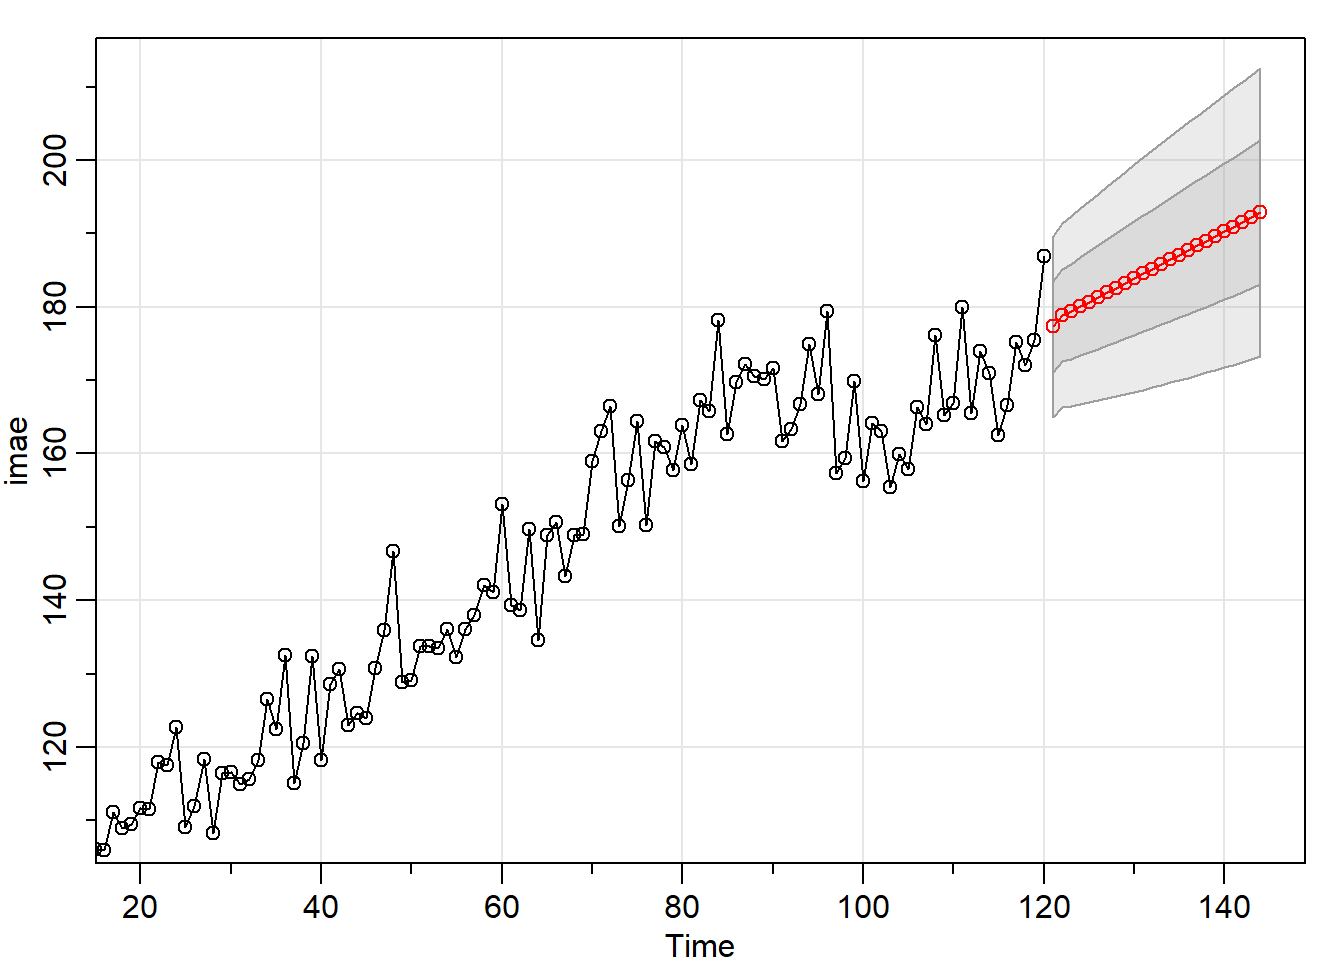
\includegraphics{index_files/figure-latex/unnamed-chunk-25-1.pdf}

\hypertarget{modelos-para-hacer-pronuxf3sticos-del-pib-de-honduras}{%
\section{Modelos para hacer pronósticos del PIB de Honduras}\label{modelos-para-hacer-pronuxf3sticos-del-pib-de-honduras}}

Modelo de regresión

\begin{Shaded}
\begin{Highlighting}[]
\FunctionTok{library}\NormalTok{(knitr)}
\FunctionTok{library}\NormalTok{(dplyr)}
\FunctionTok{library}\NormalTok{(broom) }
\FunctionTok{library}\NormalTok{(AER)}
\NormalTok{TRIM}\OtherTok{\textless{}{-}}\FunctionTok{as.xts}\NormalTok{(}\FunctionTok{read.zoo}\NormalTok{(}\StringTok{"FINAL\_HN\_P.csv"}\NormalTok{, }\AttributeTok{index.column =} \DecValTok{1}\NormalTok{, }\AttributeTok{sep =} \StringTok{";"}\NormalTok{, }\AttributeTok{header=}\ConstantTok{TRUE}\NormalTok{, }\AttributeTok{format =} \StringTok{"\%d/\%m/\%Y"}\NormalTok{))}
\NormalTok{M.ols }\OtherTok{\textless{}{-}} \FunctionTok{lm}\NormalTok{(}\FunctionTok{log}\NormalTok{(TRIM}\SpecialCharTok{$}\NormalTok{PIB) }\SpecialCharTok{\textasciitilde{}} \FunctionTok{log}\NormalTok{(TRIM}\SpecialCharTok{$}\NormalTok{PIB\_USA))}
\FunctionTok{kable}\NormalTok{(}\FunctionTok{tidy}\NormalTok{(M.ols), }\AttributeTok{digits=}\DecValTok{4}\NormalTok{, }\AttributeTok{align=}\StringTok{\textquotesingle{}c\textquotesingle{}}\NormalTok{,}\AttributeTok{caption=}\StringTok{"Regresión entre el nivel del PIB de Honduras con respecto al de USA"}\NormalTok{)}
\end{Highlighting}
\end{Shaded}

\begin{table}

\caption{\label{tab:unnamed-chunk-26}Regresión entre el nivel del PIB de Honduras con respecto al de USA}
\centering
\begin{tabular}[t]{c|c|c|c|c}
\hline
term & estimate & std.error & statistic & p.value\\
\hline
(Intercept) & -9.6056 & 0.4685 & -20.5041 & 0\\
\hline
log(TRIM\$PIB\_USA) & 2.0873 & 0.0485 & 43.0384 & 0\\
\hline
\end{tabular}
\end{table}

Modelo de regresión para el PIB de Honduras

\begin{Shaded}
\begin{Highlighting}[]
\NormalTok{INDEX  }\OtherTok{\textless{}{-}}\FunctionTok{factor}\NormalTok{(}\FunctionTok{index}\NormalTok{(TRIM))}
\NormalTok{dummies}\OtherTok{\textless{}{-}}\FunctionTok{model.matrix}\NormalTok{(}\SpecialCharTok{\textasciitilde{}}\NormalTok{INDEX)}
\NormalTok{TRIM   }\OtherTok{\textless{}{-}}\FunctionTok{merge}\NormalTok{(TRIM, dummies, }\AttributeTok{join=}\StringTok{"left"}\NormalTok{)}
\NormalTok{Y      }\OtherTok{\textless{}{-}}\FunctionTok{window}\NormalTok{(}\FunctionTok{diff}\NormalTok{(}\FunctionTok{log}\NormalTok{(TRIM}\SpecialCharTok{$}\NormalTok{PIB), }\AttributeTok{lag=}\DecValTok{4}\NormalTok{)}\SpecialCharTok{*}\DecValTok{100}\NormalTok{, }\AttributeTok{start=}\StringTok{"2004{-}03{-}01"}\NormalTok{, }\AttributeTok{end=}\StringTok{"2018{-}12{-}01"}\NormalTok{)}
\NormalTok{Y\_USA  }\OtherTok{\textless{}{-}}\FunctionTok{window}\NormalTok{(}\FunctionTok{diff}\NormalTok{(}\FunctionTok{log}\NormalTok{(TRIM}\SpecialCharTok{$}\NormalTok{PIB\_USA), }\AttributeTok{lag=}\DecValTok{4}\NormalTok{)}\SpecialCharTok{*}\DecValTok{100}\NormalTok{, }\AttributeTok{start=}\StringTok{"2004{-}03{-}01"}\NormalTok{, }\AttributeTok{end=}\StringTok{"2018{-}12{-}01"}\NormalTok{)}
\NormalTok{DUM\_HN }\OtherTok{\textless{}{-}}\FunctionTok{window}\NormalTok{(TRIM[, }\FunctionTok{c}\NormalTok{(}\StringTok{"INDEX2005.09.01"}\NormalTok{, }\StringTok{"INDEX2006.12.01"}\NormalTok{, }\StringTok{"INDEX2008.06.01"}\NormalTok{)], }\AttributeTok{start=}\StringTok{"2004{-}03{-}01"}\NormalTok{, }\AttributeTok{end=}\StringTok{"2018{-}12{-}01"}\NormalTok{)}
\NormalTok{i\_HN   }\OtherTok{\textless{}{-}}\FunctionTok{window}\NormalTok{(}\FunctionTok{diff}\NormalTok{(TRIM}\SpecialCharTok{$}\NormalTok{TASA\_P, }\AttributeTok{lag=}\DecValTok{1}\NormalTok{)}\SpecialCharTok{*}\DecValTok{100}\NormalTok{, }\AttributeTok{start=}\StringTok{"2004{-}03{-}01"}\NormalTok{, }\AttributeTok{end=}\StringTok{"2018{-}12{-}01"}\NormalTok{)}
\NormalTok{REG\_HN }\OtherTok{\textless{}{-}} \FunctionTok{merge}\NormalTok{(DUM\_HN, Y\_USA, }\AttributeTok{join=}\StringTok{"left"}\NormalTok{)}
\NormalTok{REG\_HN }\OtherTok{\textless{}{-}} \FunctionTok{merge}\NormalTok{(REG\_HN, i\_HN,  }\AttributeTok{join=}\StringTok{"left"}\NormalTok{)}
\NormalTok{PIB\_HN }\OtherTok{\textless{}{-}}\FunctionTok{sarima}\NormalTok{(Y, }\DecValTok{2}\NormalTok{,}\DecValTok{0}\NormalTok{,}\DecValTok{0}\NormalTok{,}\AttributeTok{P=}\DecValTok{1}\NormalTok{, }\AttributeTok{D=}\DecValTok{0}\NormalTok{, }\AttributeTok{Q=}\DecValTok{0}\NormalTok{, }\DecValTok{4}\NormalTok{, }\AttributeTok{xreg=}\NormalTok{REG\_HN)}
\end{Highlighting}
\end{Shaded}

\begin{verbatim}
## initial  value 0.542818 
## iter   2 value 0.399627
## iter   3 value 0.369226
## iter   4 value 0.292117
## iter   5 value 0.266433
## iter   6 value 0.252289
## iter   7 value 0.225647
## iter   8 value 0.225239
## iter   9 value 0.217205
## iter  10 value 0.210556
## iter  11 value 0.209208
## iter  12 value 0.204386
## iter  13 value 0.204299
## iter  14 value 0.204282
## iter  15 value 0.204281
## iter  16 value 0.204281
## iter  17 value 0.204281
## iter  18 value 0.204281
## iter  19 value 0.204281
## iter  19 value 0.204281
## iter  19 value 0.204281
## final  value 0.204281 
## converged
## initial  value 0.186966 
## iter   2 value 0.186057
## iter   3 value 0.185621
## iter   4 value 0.185490
## iter   5 value 0.185264
## iter   6 value 0.185174
## iter   7 value 0.185124
## iter   8 value 0.185091
## iter   9 value 0.185069
## iter  10 value 0.185068
## iter  11 value 0.185068
## iter  12 value 0.185068
## iter  13 value 0.185068
## iter  13 value 0.185068
## iter  13 value 0.185068
## final  value 0.185068 
## converged
\end{verbatim}

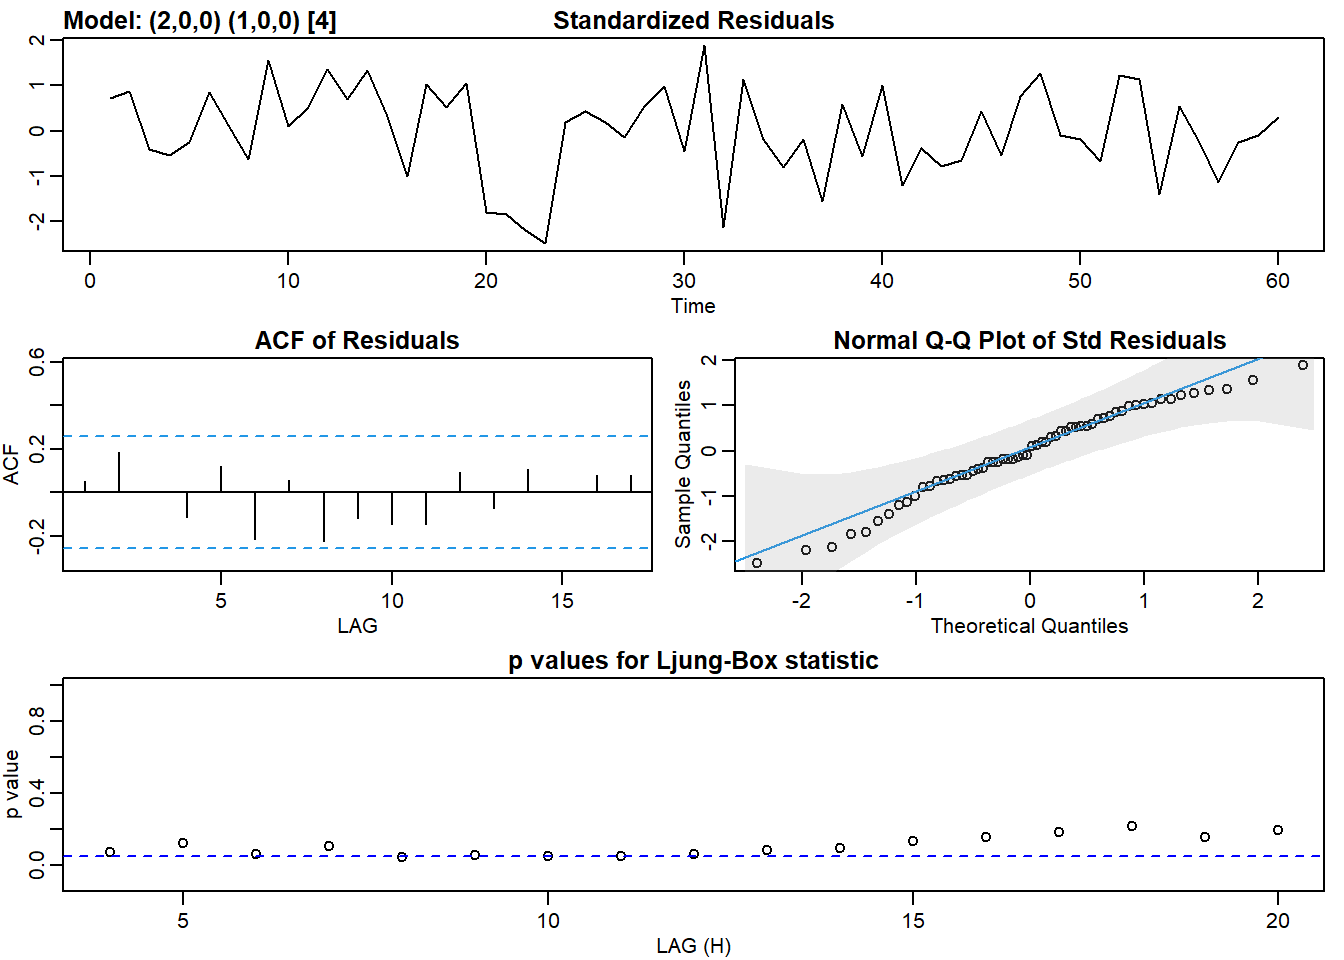
\includegraphics{index_files/figure-latex/unnamed-chunk-27-1.pdf}

\begin{Shaded}
\begin{Highlighting}[]
\NormalTok{PIB\_HN}\SpecialCharTok{$}\NormalTok{ttable}
\end{Highlighting}
\end{Shaded}

\begin{verbatim}
##                 Estimate     SE t.value p.value
## ar1               0.5867 0.1333  4.4015  0.0001
## ar2               0.2160 0.1364  1.5839  0.1194
## sar1             -0.3799 0.1277 -2.9750  0.0045
## intercept         2.4738 0.6710  3.6869  0.0006
## INDEX2005.09.01   3.3296 0.9658  3.4473  0.0011
## INDEX2006.12.01   2.0824 1.0148  2.0521  0.0453
## INDEX2008.06.01   2.2639 1.0536  2.1487  0.0364
## PIB_USA           0.7381 0.1920  3.8438  0.0003
## TASA_P            0.0056 0.0028  1.9794  0.0532
\end{verbatim}

Modelo de regresión para el PIB de USA

\begin{Shaded}
\begin{Highlighting}[]
\NormalTok{Y\_USA     }\OtherTok{\textless{}{-}}\FunctionTok{window}\NormalTok{(}\FunctionTok{diff}\NormalTok{(}\FunctionTok{log}\NormalTok{(TRIM}\SpecialCharTok{$}\NormalTok{PIB\_USA), }\AttributeTok{lag=}\DecValTok{4}\NormalTok{)}\SpecialCharTok{*}\DecValTok{100}\NormalTok{, }\AttributeTok{start=}\StringTok{"1990{-}03{-}01"}\NormalTok{, }\AttributeTok{end=}\StringTok{"2018{-}12{-}01"}\NormalTok{)}
\NormalTok{DUM\_USA   }\OtherTok{\textless{}{-}}\FunctionTok{window}\NormalTok{(TRIM[, }\FunctionTok{c}\NormalTok{(}\StringTok{"INDEX2008.12.01"}\NormalTok{, }\StringTok{"INDEX2009.12.01"}\NormalTok{)], }\AttributeTok{start=}\StringTok{"1990{-}03{-}01"}\NormalTok{, }\AttributeTok{end=}\StringTok{"2018{-}12{-}01"}\NormalTok{)}
\NormalTok{PIB\_USA   }\OtherTok{\textless{}{-}}\FunctionTok{sarima}\NormalTok{(Y\_USA, }\DecValTok{2}\NormalTok{,}\DecValTok{0}\NormalTok{,}\DecValTok{0}\NormalTok{,}\AttributeTok{P=}\DecValTok{1}\NormalTok{, }\AttributeTok{D=}\DecValTok{0}\NormalTok{, }\AttributeTok{Q=}\DecValTok{0}\NormalTok{, }\DecValTok{4}\NormalTok{, }\AttributeTok{xreg=}\NormalTok{DUM\_USA )}
\end{Highlighting}
\end{Shaded}

\begin{verbatim}
## initial  value 0.434672 
## iter   2 value 0.189957
## iter   3 value 0.021610
## iter   4 value -0.116248
## iter   5 value -0.251754
## iter   6 value -0.332615
## iter   7 value -0.410324
## iter   8 value -0.433150
## iter   9 value -0.436896
## iter  10 value -0.439417
## iter  11 value -0.440979
## iter  12 value -0.441051
## iter  13 value -0.441096
## iter  14 value -0.441109
## iter  15 value -0.441110
## iter  16 value -0.441110
## iter  17 value -0.441111
## iter  18 value -0.441115
## iter  19 value -0.441117
## iter  20 value -0.441118
## iter  21 value -0.441119
## iter  22 value -0.441119
## iter  22 value -0.441119
## iter  22 value -0.441119
## final  value -0.441119 
## converged
\end{verbatim}

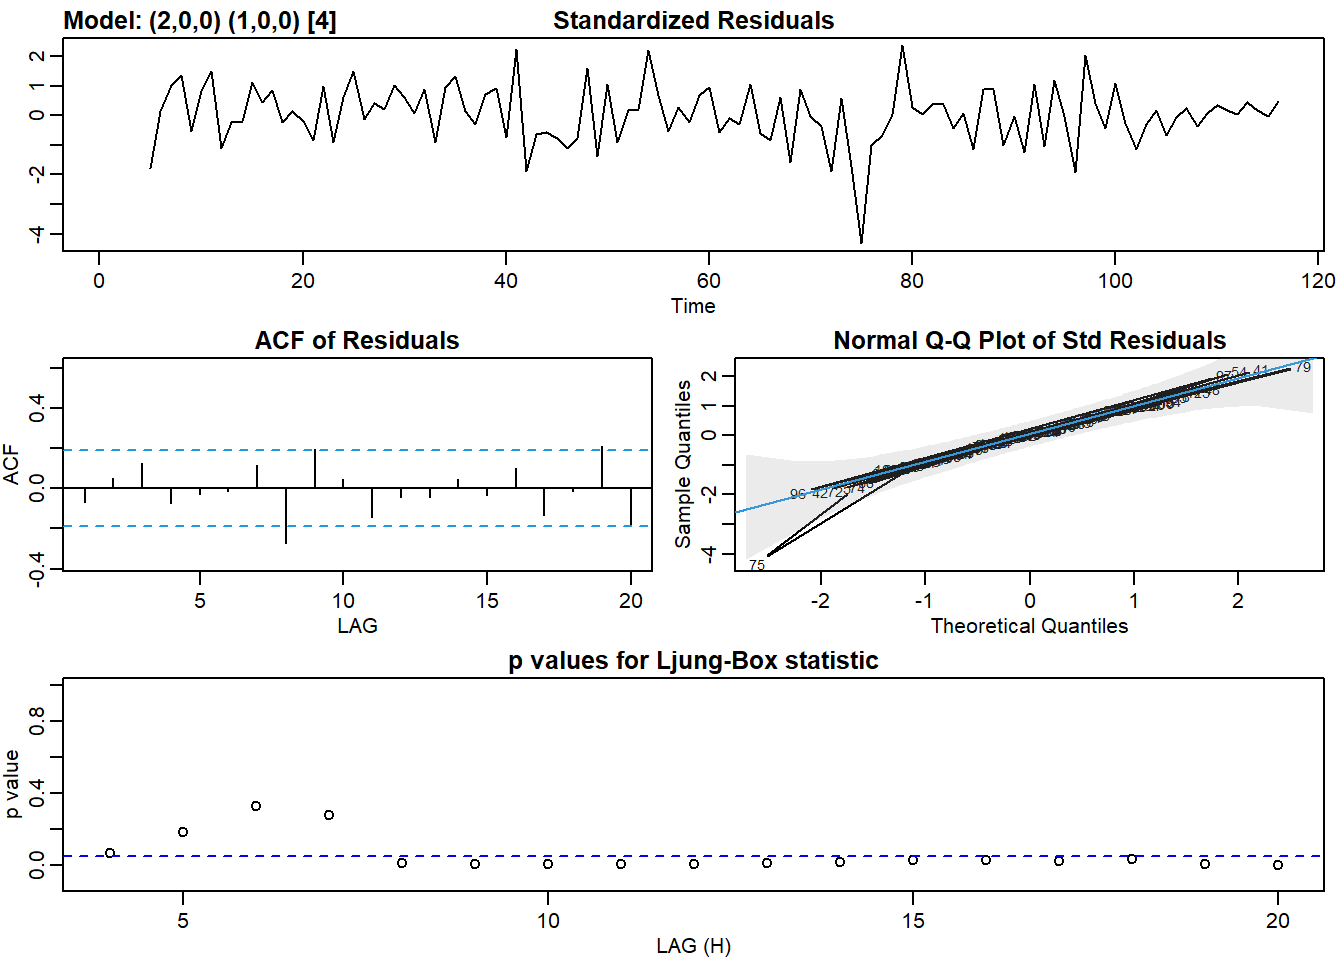
\includegraphics{index_files/figure-latex/unnamed-chunk-28-1.pdf}

\begin{Shaded}
\begin{Highlighting}[]
\NormalTok{PIB\_USA}\SpecialCharTok{$}\NormalTok{ttable}
\end{Highlighting}
\end{Shaded}

\begin{verbatim}
##                 Estimate     SE t.value p.value
## ar1               1.2831 0.0888 14.4513  0.0000
## ar2              -0.3694 0.0899 -4.1111  0.0001
## sar1             -0.3721 0.0925 -4.0228  0.0001
## intercept         2.4027 0.4862  4.9417  0.0000
## INDEX2008.12.01   0.3768 0.3851  0.9784  0.3301
## INDEX2009.12.01  -0.1896 0.3823 -0.4958  0.6210
\end{verbatim}

Pronóstico del PIB de USA

\begin{Shaded}
\begin{Highlighting}[]
\NormalTok{DUM\_USA\_N }\OtherTok{\textless{}{-}}\FunctionTok{window}\NormalTok{(TRIM[, }\FunctionTok{c}\NormalTok{(}\StringTok{"INDEX2008.12.01"}\NormalTok{, }\StringTok{"INDEX2009.12.01"}\NormalTok{)], }\AttributeTok{start=}\StringTok{"2019{-}03{-}01"}\NormalTok{, }\AttributeTok{end=}\StringTok{"2022{-}12{-}01"}\NormalTok{)}
\NormalTok{Y\_USA\_N   }\OtherTok{\textless{}{-}}\FunctionTok{sarima.for}\NormalTok{(Y\_USA,}\DecValTok{16}\NormalTok{,}\DecValTok{2}\NormalTok{,}\DecValTok{0}\NormalTok{,}\DecValTok{0}\NormalTok{,}\DecValTok{1}\NormalTok{,}\DecValTok{0}\NormalTok{,}\DecValTok{0}\NormalTok{,}\DecValTok{4}\NormalTok{, }\AttributeTok{xreg=}\NormalTok{DUM\_USA, }\AttributeTok{newxreg=}\NormalTok{DUM\_USA\_N) }
\end{Highlighting}
\end{Shaded}

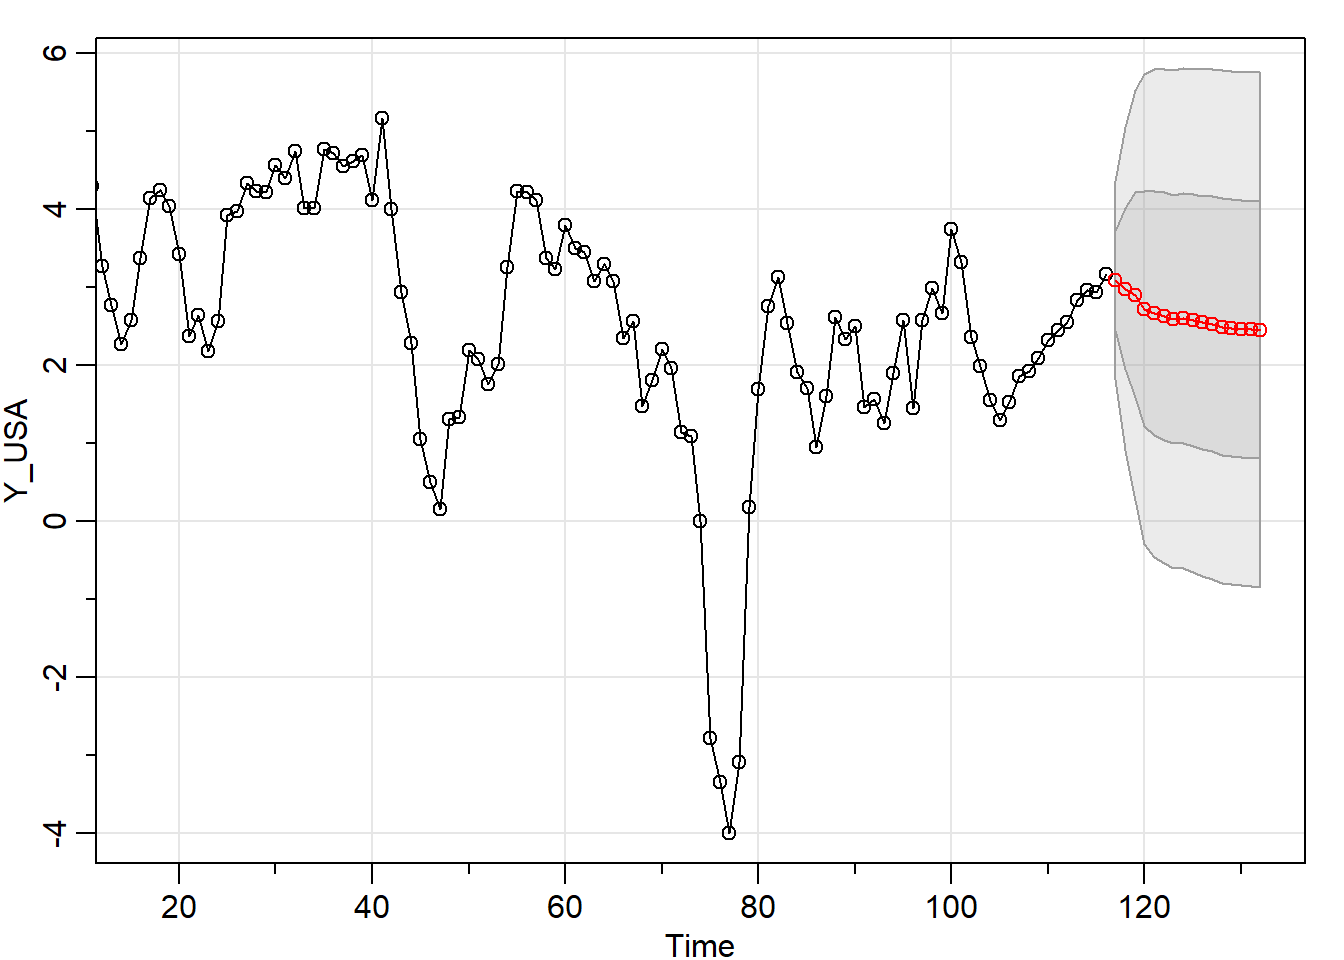
\includegraphics{index_files/figure-latex/unnamed-chunk-29-1.pdf}

Pronóstico del PIB de Honduras

\begin{Shaded}
\begin{Highlighting}[]
\NormalTok{dates }\OtherTok{\textless{}{-}} \FunctionTok{seq}\NormalTok{(}\FunctionTok{as.Date}\NormalTok{(}\StringTok{"2019{-}03{-}01"}\NormalTok{), }\AttributeTok{length =} \DecValTok{16}\NormalTok{, }\AttributeTok{by =} \StringTok{"quarter"}\NormalTok{)}
\NormalTok{DUM\_HN\_N }\OtherTok{\textless{}{-}}\FunctionTok{window}\NormalTok{(TRIM[, }\FunctionTok{c}\NormalTok{(}\StringTok{"INDEX2005.09.01"}\NormalTok{, }\StringTok{"INDEX2006.12.01"}\NormalTok{, }\StringTok{"INDEX2008.06.01"}\NormalTok{)], }\AttributeTok{start=}\StringTok{"2019{-}03{-}01"}\NormalTok{, }\AttributeTok{end=}\StringTok{"2022{-}12{-}01"}\NormalTok{)}
\NormalTok{Y\_USA\_N   }\OtherTok{\textless{}{-}} \FunctionTok{xts}\NormalTok{(}\AttributeTok{x=}\NormalTok{Y\_USA\_N}\SpecialCharTok{$}\NormalTok{pred, }\AttributeTok{order.by =}\NormalTok{ dates)}
\NormalTok{REG\_HN\_N}\OtherTok{\textless{}{-}} \FunctionTok{merge}\NormalTok{(DUM\_HN\_N, Y\_USA\_N, }\AttributeTok{join=}\StringTok{"left"}\NormalTok{)}
\NormalTok{data }\OtherTok{\textless{}{-}} \FunctionTok{rep}\NormalTok{(}\DecValTok{1}\NormalTok{, }\DecValTok{16}\NormalTok{)}
\NormalTok{i\_HN\_N }\OtherTok{=} \FunctionTok{xts}\NormalTok{(}\AttributeTok{x =}\NormalTok{ data, }\AttributeTok{order.by =}\NormalTok{ dates)}
\NormalTok{REG\_HN\_N}\OtherTok{\textless{}{-}} \FunctionTok{merge}\NormalTok{(REG\_HN\_N, i\_HN\_N, }\AttributeTok{join=}\StringTok{"left"}\NormalTok{)}
\NormalTok{Y\_N}\OtherTok{\textless{}{-}}\FunctionTok{sarima.for}\NormalTok{(Y,}\DecValTok{16}\NormalTok{,}\DecValTok{2}\NormalTok{,}\DecValTok{0}\NormalTok{,}\DecValTok{0}\NormalTok{,}\DecValTok{1}\NormalTok{,}\DecValTok{0}\NormalTok{,}\DecValTok{0}\NormalTok{,}\DecValTok{4}\NormalTok{, }\AttributeTok{xreg=}\NormalTok{REG\_HN, }\AttributeTok{newxreg=}\NormalTok{REG\_HN\_N) }
\end{Highlighting}
\end{Shaded}

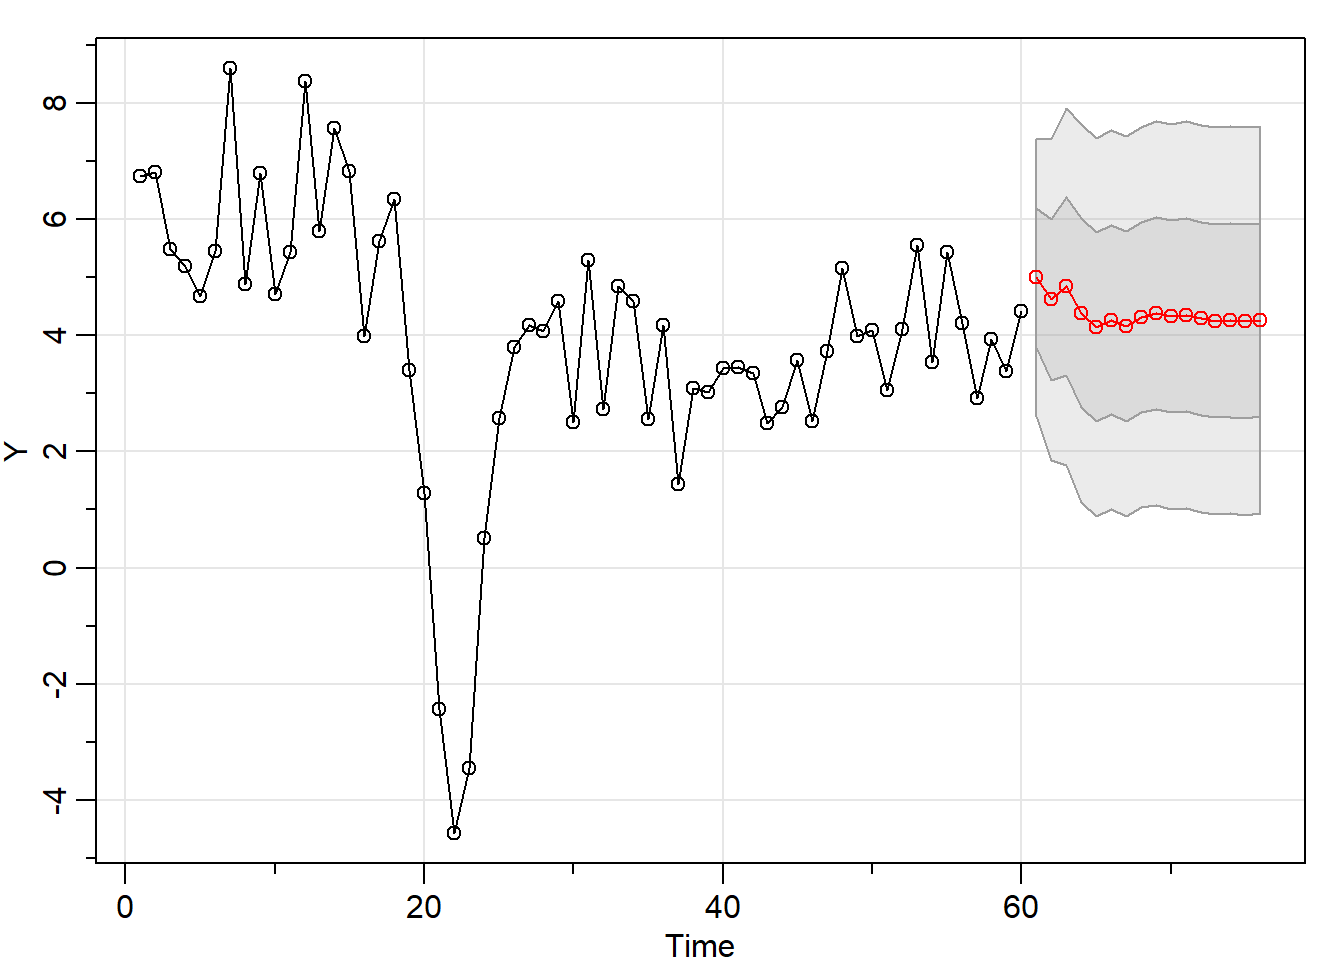
\includegraphics{index_files/figure-latex/unnamed-chunk-30-1.pdf}

\hypertarget{simulaciuxf3n-de-shock-en-el-pib-de-usa}{%
\section{Simulación de shock en el PIB de USA}\label{simulaciuxf3n-de-shock-en-el-pib-de-usa}}

Simulación

\begin{Shaded}
\begin{Highlighting}[]
\NormalTok{dates }\OtherTok{\textless{}{-}} \FunctionTok{seq}\NormalTok{(}\FunctionTok{as.Date}\NormalTok{(}\StringTok{"2019{-}03{-}01"}\NormalTok{), }\AttributeTok{length =} \DecValTok{16}\NormalTok{, }\AttributeTok{by =} \StringTok{"quarter"}\NormalTok{)}
\NormalTok{shock }\OtherTok{\textless{}{-}}\FunctionTok{c}\NormalTok{()}
\NormalTok{shock[}\DecValTok{1}\NormalTok{]}\OtherTok{\textless{}{-}} \DecValTok{0}
\NormalTok{shock[}\DecValTok{2}\NormalTok{]}\OtherTok{\textless{}{-}} \SpecialCharTok{{-}}\DecValTok{3}\SpecialCharTok{*}\NormalTok{(}\DecValTok{1}\SpecialCharTok{/{-}}\FloatTok{0.1896}\NormalTok{)}
\ControlFlowTok{for}\NormalTok{(i }\ControlFlowTok{in} \DecValTok{3}\SpecialCharTok{:}\DecValTok{16}\NormalTok{ )\{}
\NormalTok{  shock[i]}\OtherTok{\textless{}{-}}\FloatTok{0.85}\SpecialCharTok{*}\NormalTok{shock[i}\DecValTok{{-}1}\NormalTok{]}
\NormalTok{\}}
\NormalTok{shock\_Y\_USA}\OtherTok{=} \FunctionTok{xts}\NormalTok{(}\AttributeTok{x =}\NormalTok{ shock, }\AttributeTok{order.by =}\NormalTok{ dates) }
\NormalTok{REG\_SHOCK}\OtherTok{\textless{}{-}}\FunctionTok{window}\NormalTok{(TRIM[, }\FunctionTok{c}\NormalTok{(}\StringTok{"INDEX2008.12.01"}\NormalTok{)], }\AttributeTok{start=}\StringTok{"2019{-}03{-}01"}\NormalTok{, }\AttributeTok{end=}\StringTok{"2022{-}12{-}01"}\NormalTok{)}
\NormalTok{REG\_SHOCK}\OtherTok{\textless{}{-}} \FunctionTok{merge}\NormalTok{(REG\_SHOCK, shock\_Y\_USA, }\AttributeTok{join=}\StringTok{"left"}\NormalTok{)}
\NormalTok{Y\_USA\_SHOCK}\OtherTok{\textless{}{-}}\FunctionTok{sarima.for}\NormalTok{(Y\_USA,}\DecValTok{16}\NormalTok{,}\DecValTok{2}\NormalTok{,}\DecValTok{0}\NormalTok{,}\DecValTok{0}\NormalTok{,}\DecValTok{1}\NormalTok{,}\DecValTok{0}\NormalTok{,}\DecValTok{0}\NormalTok{,}\DecValTok{4}\NormalTok{, }\AttributeTok{xreg=}\NormalTok{DUM\_USA, }\AttributeTok{newxreg=}\NormalTok{REG\_SHOCK) }
\end{Highlighting}
\end{Shaded}

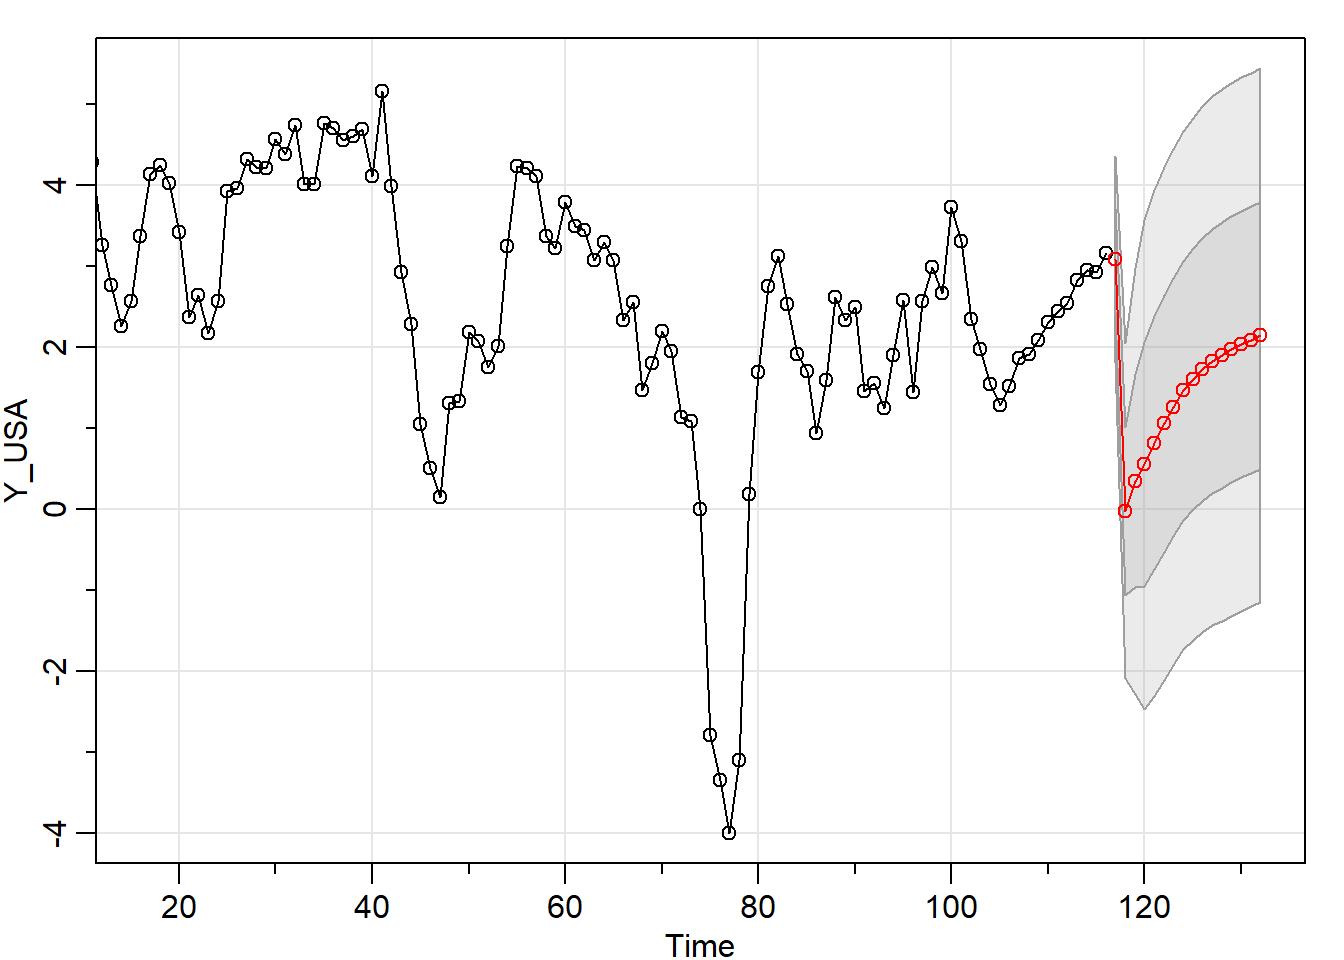
\includegraphics{index_files/figure-latex/unnamed-chunk-31-1.pdf}

Transimisión del shock al PIB de Honduras

\begin{Shaded}
\begin{Highlighting}[]
\NormalTok{Y\_USA\_S }\OtherTok{\textless{}{-}} \FunctionTok{xts}\NormalTok{(}\AttributeTok{x=}\NormalTok{Y\_USA\_SHOCK}\SpecialCharTok{$}\NormalTok{pred, }\AttributeTok{order.by =}\NormalTok{ dates)}
\NormalTok{REG\_HN\_S}\OtherTok{\textless{}{-}} \FunctionTok{merge}\NormalTok{(DUM\_HN\_N, Y\_USA\_S, }\AttributeTok{join=}\StringTok{"left"}\NormalTok{)}
\NormalTok{REG\_HN\_S}\OtherTok{\textless{}{-}} \FunctionTok{merge}\NormalTok{(REG\_HN\_S, i\_HN\_N, }\AttributeTok{join=}\StringTok{"left"}\NormalTok{)}
\NormalTok{Y\_S}\OtherTok{\textless{}{-}}      \FunctionTok{sarima.for}\NormalTok{(Y,}\DecValTok{16}\NormalTok{,}\DecValTok{2}\NormalTok{,}\DecValTok{0}\NormalTok{,}\DecValTok{0}\NormalTok{,}\DecValTok{1}\NormalTok{,}\DecValTok{0}\NormalTok{,}\DecValTok{0}\NormalTok{,}\DecValTok{4}\NormalTok{, }\AttributeTok{xreg=}\NormalTok{REG\_HN, }\AttributeTok{newxreg=}\NormalTok{REG\_HN\_S) }
\end{Highlighting}
\end{Shaded}

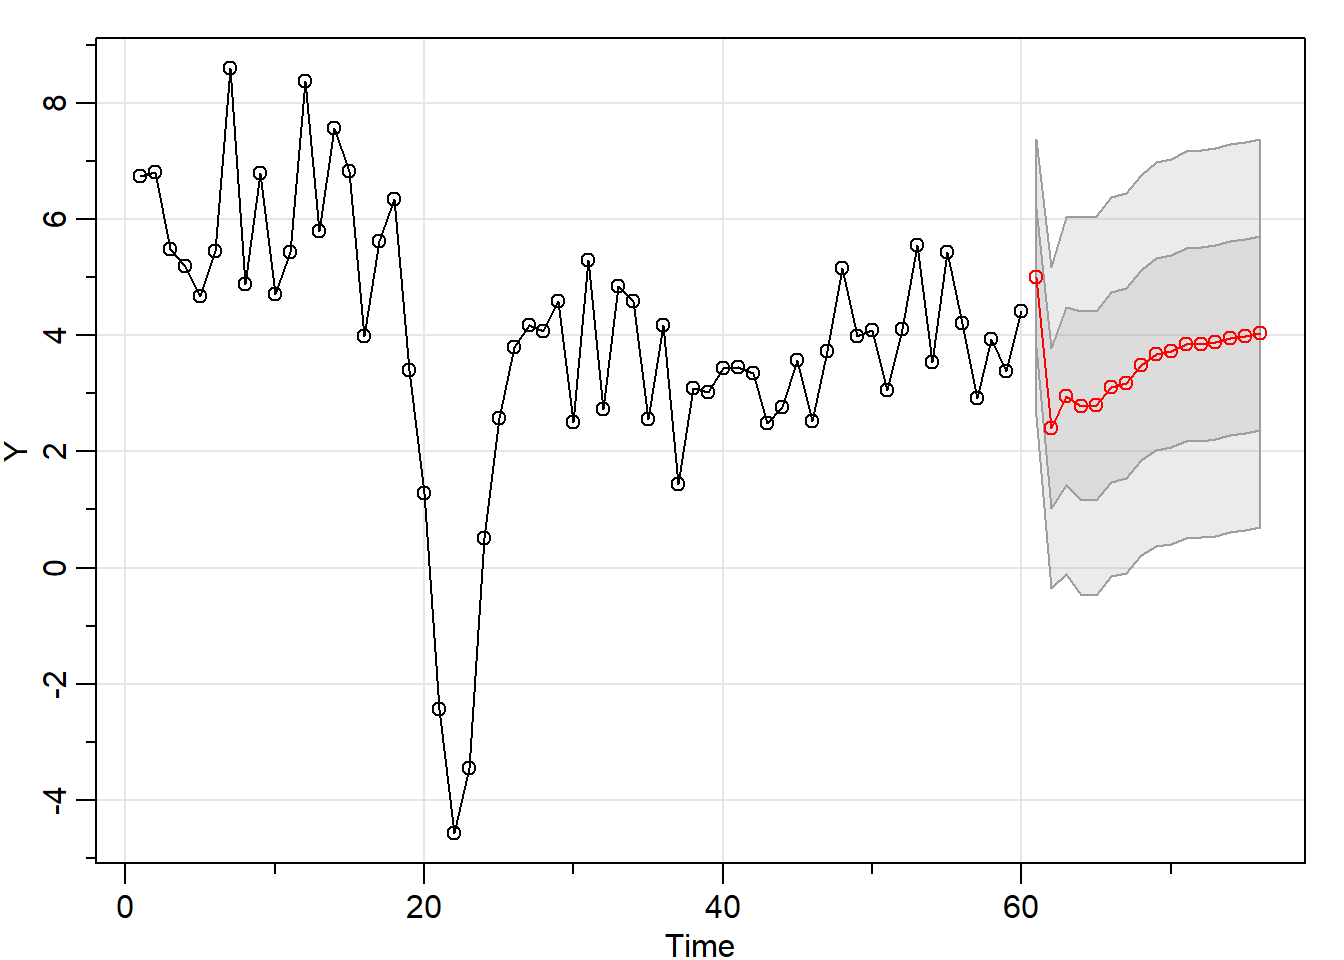
\includegraphics{index_files/figure-latex/unnamed-chunk-32-1.pdf}

\hypertarget{ejercicio-fuera-de-muestra}{%
\chapter{Ejercicio fuera de muestra}\label{ejercicio-fuera-de-muestra}}

\hypertarget{aplicaciuxf3n-sobre-la-inflaciuxf3n-de-honduras}{%
\section{Aplicación sobre la inflación de Honduras}\label{aplicaciuxf3n-sobre-la-inflaciuxf3n-de-honduras}}

Los pronósticos de inflación a determinado horizonte h, realizados en el momento t a partir de una determinada especificación econométrica j (\(\hat{\pi}_{t+h\mid t}^{j}\)) son comparados con los datos efectivos (\(\pi_{t+h}\)), deduciendo los errores de pronósticos (\(E_{t+h}^{j}\)) en conformidad a la ecuación \label{eq:1} la cual aplica para cualquier tipo de ventana \(h\).

\begin{equation} 
 ECM_{h}^{j}=\frac{\sum\limits_{n=0}^{N=g_{h}-1} (E_{t+h+n}^{j})^{2}}{g_{h}}
 \label{eq:1}
\end{equation}

En el siguiente código, se seleccionará la mejor específicación según el criterio de información Akaike (AIC) para la inflación de Honduras tomando como muestra enero 1994 a diciembre 2006.

\begin{Shaded}
\begin{Highlighting}[]
\FunctionTok{library}\NormalTok{(}\StringTok{"xts"}\NormalTok{) }
\FunctionTok{library}\NormalTok{(}\StringTok{"zoo"}\NormalTok{)}
\FunctionTok{library}\NormalTok{(}\StringTok{"astsa"}\NormalTok{)}
\FunctionTok{library}\NormalTok{(}\StringTok{"forecast"}\NormalTok{)}
\FunctionTok{library}\NormalTok{(}\StringTok{"ggplot2"}\NormalTok{)}
\FunctionTok{library}\NormalTok{(}\StringTok{"forecast"}\NormalTok{)}
\FunctionTok{library}\NormalTok{(}\StringTok{"ggfortify"}\NormalTok{)}
\FunctionTok{library}\NormalTok{(}\StringTok{"stargazer"}\NormalTok{)}
\FunctionTok{library}\NormalTok{(}\StringTok{"urca"}\NormalTok{)}
\FunctionTok{library}\NormalTok{(}\StringTok{"dynlm"}\NormalTok{)}
\FunctionTok{library}\NormalTok{(}\StringTok{"scales"}\NormalTok{)}
\FunctionTok{library}\NormalTok{(}\StringTok{"quantmod"}\NormalTok{)}
\FunctionTok{library}\NormalTok{(}\StringTok{"dplyr"}\NormalTok{)}
\FunctionTok{library}\NormalTok{(}\StringTok{"sandwich"}\NormalTok{)}
\FunctionTok{library}\NormalTok{(}\StringTok{"knitr"}\NormalTok{) }
\FunctionTok{library}\NormalTok{(}\StringTok{"dynlm"}\NormalTok{)}
\FunctionTok{library}\NormalTok{(}\StringTok{"stargazer"}\NormalTok{)}
\NormalTok{MES}\OtherTok{\textless{}{-}}\FunctionTok{as.xts}\NormalTok{(}\FunctionTok{read.zoo}\NormalTok{(}\StringTok{"MES\_HN.csv"}\NormalTok{, }\AttributeTok{index.column =} \DecValTok{1}\NormalTok{, }\AttributeTok{sep =} \StringTok{";"}\NormalTok{, }\AttributeTok{header=}\ConstantTok{TRUE}\NormalTok{, }\AttributeTok{format =} \StringTok{"\%d/\%m/\%Y"}\NormalTok{))}
\NormalTok{INFLA }\OtherTok{\textless{}{-}}\NormalTok{(}\FunctionTok{log}\NormalTok{(MES}\SpecialCharTok{$}\NormalTok{IPC)}\SpecialCharTok{{-}}\NormalTok{stats}\SpecialCharTok{::}\FunctionTok{lag}\NormalTok{(}\FunctionTok{log}\NormalTok{(MES}\SpecialCharTok{$}\NormalTok{IPC), }\AttributeTok{n=}\DecValTok{12}\NormalTok{))}\SpecialCharTok{/}\NormalTok{stats}\SpecialCharTok{::}\FunctionTok{lag}\NormalTok{(}\FunctionTok{log}\NormalTok{(MES}\SpecialCharTok{$}\NormalTok{IPC), }\AttributeTok{n=}\DecValTok{12}\NormalTok{)}
\NormalTok{INFLA1}\OtherTok{\textless{}{-}}\NormalTok{INFLA[}\StringTok{"1994{-}01{-}01/2006{-}12{-}01"}\NormalTok{]}
\NormalTok{INFLA\_fit }\OtherTok{\textless{}{-}}\FunctionTok{auto.arima}\NormalTok{(INFLA1, }\AttributeTok{ic =} \FunctionTok{c}\NormalTok{(}\StringTok{"aic"}\NormalTok{))}
\NormalTok{INFLA\_fit}
\end{Highlighting}
\end{Shaded}

\begin{verbatim}
## Series: INFLA1 
## ARIMA(1,1,2) with drift 
## 
## Coefficients:
##           ar1      ma1      ma2  drift
##       -0.6503  -0.1120  -0.7132  0e+00
## s.e.   0.1504   0.1212   0.1035  1e-04
## 
## sigma^2 estimated as 2.125e-06:  log likelihood=793.57
## AIC=-1577.13   AICc=-1576.73   BIC=-1561.91
\end{verbatim}

La mejor específicación seleccionada es un a ARIMA(1,1,2). El que formalmente puede escribirse como:

\begin{equation} 
\Phi(L)(1-L)\pi_{t}=\Theta(L)\epsilon_{t}
\label{eq:3}
\end{equation}

Donde \(\Phi(L)=(1+0.65L),\) \(\Theta(L)=(1-0.11L-0.71L^{2})\).

Luego de tener esa específicación podemos comparar su desempeño predictivo con respecto a los datos observados que se encuentran \emph{fuera de la muestra de estimación}.

Para ejemplificar se selecciona como horizonte predictivo 3 meses.

\begin{Shaded}
\begin{Highlighting}[]
\NormalTok{FECHA            }\OtherTok{\textless{}{-}}\FunctionTok{index}\NormalTok{(MES)}
\NormalTok{t\_inicial        }\OtherTok{\textless{}{-}}\FunctionTok{first}\NormalTok{(FECHA,}\StringTok{\textquotesingle{}1 month\textquotesingle{}}\NormalTok{)}
\NormalTok{index\_final      }\OtherTok{\textless{}{-}}\FunctionTok{last}\NormalTok{(}\FunctionTok{index}\NormalTok{(FECHA))}
\NormalTok{fecha\_contador   }\OtherTok{\textless{}{-}}\FunctionTok{seq}\NormalTok{(}\FunctionTok{as.Date}\NormalTok{(t\_inicial), }\AttributeTok{length =}\NormalTok{index\_final, }\AttributeTok{by =} \StringTok{"months"}\NormalTok{)}
\NormalTok{counter          }\OtherTok{\textless{}{-}}\FunctionTok{c}\NormalTok{(}\DecValTok{1}\SpecialCharTok{:}\NormalTok{index\_final)  }
\NormalTok{contador         }\OtherTok{\textless{}{-}}\FunctionTok{xts}\NormalTok{(}\AttributeTok{x=}\NormalTok{counter, }\AttributeTok{order.by =}\NormalTok{ fecha\_contador)}
\NormalTok{inicio\_estimacion}\OtherTok{\textless{}{-}}\FunctionTok{coredata}\NormalTok{(contador[}\StringTok{"1994{-}01{-}01"}\NormalTok{])[}\DecValTok{1}\NormalTok{]}
\NormalTok{final\_estimacion }\OtherTok{\textless{}{-}}\FunctionTok{coredata}\NormalTok{(contador[}\StringTok{"2006{-}12{-}01"}\NormalTok{])[}\DecValTok{1}\NormalTok{]}
\NormalTok{final\_muestra    }\OtherTok{\textless{}{-}}\FunctionTok{coredata}\NormalTok{(contador[}\StringTok{"2019{-}02{-}01"}\NormalTok{])[}\DecValTok{1}\NormalTok{]}
\NormalTok{H                }\OtherTok{\textless{}{-}}\DecValTok{3} \CommentTok{\#Horizonte predictivo}
\NormalTok{DENTRO           }\OtherTok{\textless{}{-}} \FunctionTok{seq}\NormalTok{(}\FunctionTok{as.Date}\NormalTok{(FECHA[inicio\_estimacion]), }
\AttributeTok{length =}\NormalTok{final\_estimacion}\SpecialCharTok{+}\NormalTok{H}\SpecialCharTok{{-}}\NormalTok{inicio\_estimacion, }\AttributeTok{by =} \StringTok{"months"}\NormalTok{)}
\NormalTok{FUERA            }\OtherTok{\textless{}{-}} \FunctionTok{seq}\NormalTok{(}\FunctionTok{as.Date}\NormalTok{(FECHA[final\_estimacion}\SpecialCharTok{+}\DecValTok{1}\NormalTok{]), }
\AttributeTok{length =}\NormalTok{final\_muestra}\SpecialCharTok{{-}}\NormalTok{H}\SpecialCharTok{{-}}\NormalTok{final\_estimacion, }\AttributeTok{by =} \StringTok{"months"}\NormalTok{)}
\FunctionTok{assign}\NormalTok{(}\FunctionTok{paste}\NormalTok{(}\StringTok{\textquotesingle{}PI\_\textquotesingle{}}\NormalTok{, H, }\AttributeTok{sep=}\StringTok{\textquotesingle{}\textquotesingle{}}\NormalTok{), }\FunctionTok{xts}\NormalTok{(}\AttributeTok{x=}\FunctionTok{window}\NormalTok{(INFLA, }\AttributeTok{start=}\NormalTok{FECHA[inicio\_estimacion], }\AttributeTok{end=}\NormalTok{FECHA[final\_estimacion}\SpecialCharTok{+}\NormalTok{H}\DecValTok{{-}1}\NormalTok{]),}
\AttributeTok{order.by =}\NormalTok{ DENTRO))}
\NormalTok{Y }\OtherTok{\textless{}{-}}\FunctionTok{window}\NormalTok{(INFLA, }\AttributeTok{start=}\NormalTok{FECHA[inicio\_estimacion], }\AttributeTok{end=}\NormalTok{FECHA[final\_estimacion])}
\ControlFlowTok{for}\NormalTok{(i }\ControlFlowTok{in} \DecValTok{1}\SpecialCharTok{:}\FunctionTok{length}\NormalTok{(FUERA))\{}
\NormalTok{Y\_F}\OtherTok{\textless{}{-}}\FunctionTok{sarima.for}\NormalTok{(Y,H,}\DecValTok{1}\NormalTok{,}\DecValTok{1}\NormalTok{,}\DecValTok{2}\NormalTok{, }\AttributeTok{xreg=}\ConstantTok{NULL}\NormalTok{, }
                \AttributeTok{newxreg=}\ConstantTok{NULL}\NormalTok{, }\AttributeTok{plot=} \ConstantTok{FALSE}\NormalTok{) }
\NormalTok{dates\_out}\OtherTok{\textless{}{-}}\FunctionTok{as.Date}\NormalTok{(FECHA[final\_estimacion}\SpecialCharTok{+}\NormalTok{i}\SpecialCharTok{+}\NormalTok{H}\DecValTok{{-}1}\NormalTok{])}
\NormalTok{Y\_F\_P}\OtherTok{\textless{}{-}}\FunctionTok{xts}\NormalTok{(}\AttributeTok{x=}\NormalTok{Y\_F}\SpecialCharTok{$}\NormalTok{pred[H], }\AttributeTok{order.by =}\NormalTok{ dates\_out)}
\NormalTok{DENTRO}\OtherTok{\textless{}{-}}\FunctionTok{seq}\NormalTok{(}\FunctionTok{as.Date}\NormalTok{(FECHA[inicio\_estimacion]), }
\AttributeTok{length =}\NormalTok{final\_estimacion}\SpecialCharTok{+}\DecValTok{1}\SpecialCharTok{+}\NormalTok{i}\SpecialCharTok{{-}}\NormalTok{inicio\_estimacion, }\AttributeTok{by =} \StringTok{"months"}\NormalTok{)}
\NormalTok{Y }\OtherTok{\textless{}{-}}\FunctionTok{window}\NormalTok{(INFLA, }\AttributeTok{start=}\NormalTok{FECHA[inicio\_estimacion], }\AttributeTok{end=}\NormalTok{FECHA[final\_estimacion}\SpecialCharTok{+}\NormalTok{i])}
\FunctionTok{assign}\NormalTok{(}\FunctionTok{paste}\NormalTok{(}\StringTok{\textquotesingle{}PI\_\textquotesingle{}}\NormalTok{, H, }\AttributeTok{sep=}\StringTok{\textquotesingle{}\textquotesingle{}}\NormalTok{),}\FunctionTok{rbind}\NormalTok{(}\FunctionTok{get}\NormalTok{(}\FunctionTok{paste}\NormalTok{(}\StringTok{\textquotesingle{}PI\_\textquotesingle{}}\NormalTok{, H, }\AttributeTok{sep=}\StringTok{\textquotesingle{}\textquotesingle{}}\NormalTok{)), }
\NormalTok{Y\_F\_P))}
\NormalTok{\}}
\end{Highlighting}
\end{Shaded}

\includegraphics{03_EJERCICIOS_files/figure-latex/unnamed-chunk-2-1.pdf} 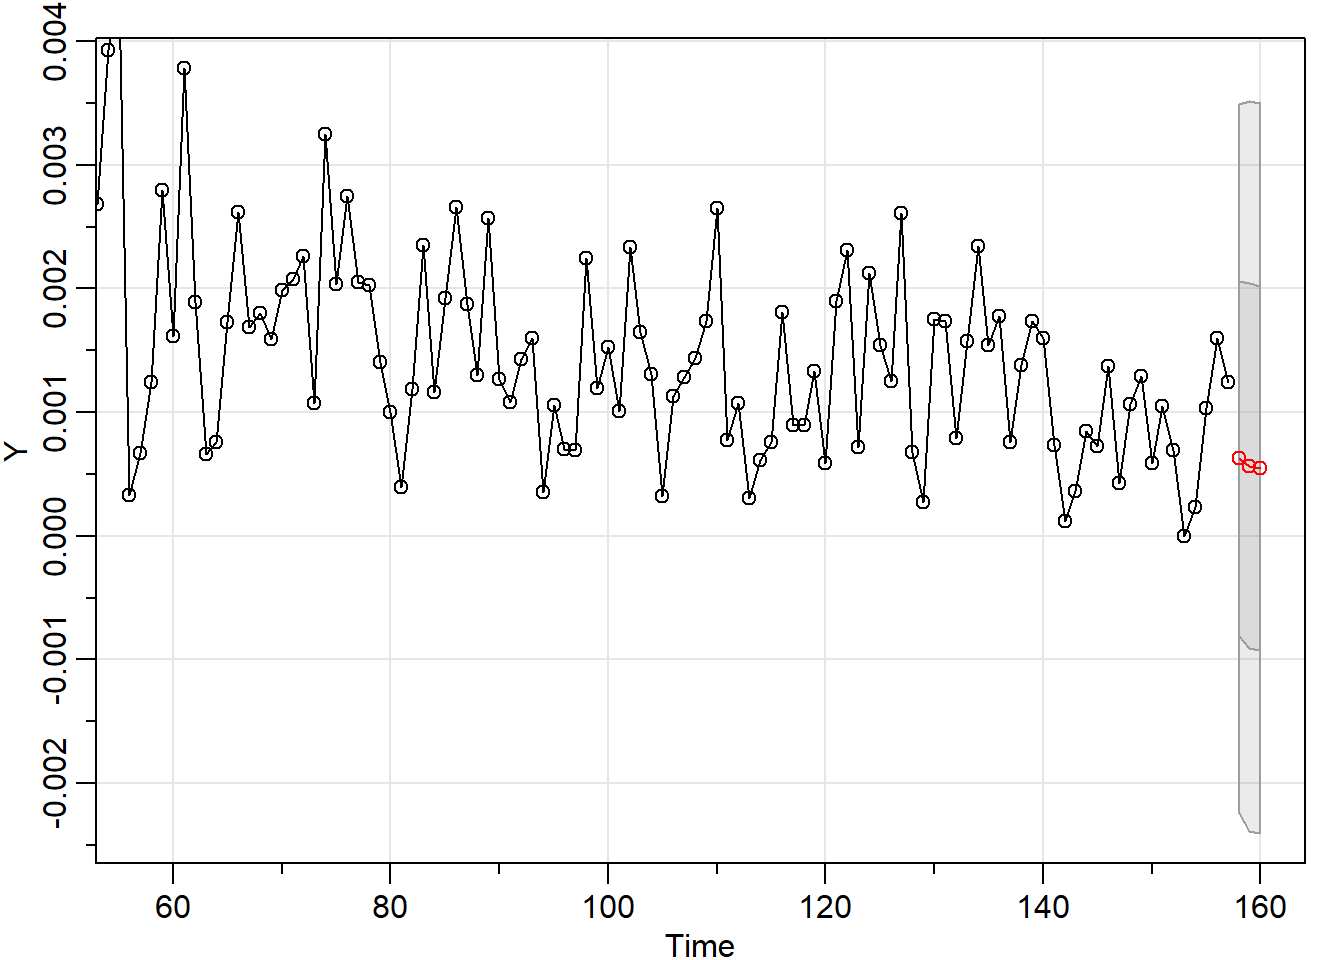
\includegraphics{03_EJERCICIOS_files/figure-latex/unnamed-chunk-2-2.pdf} 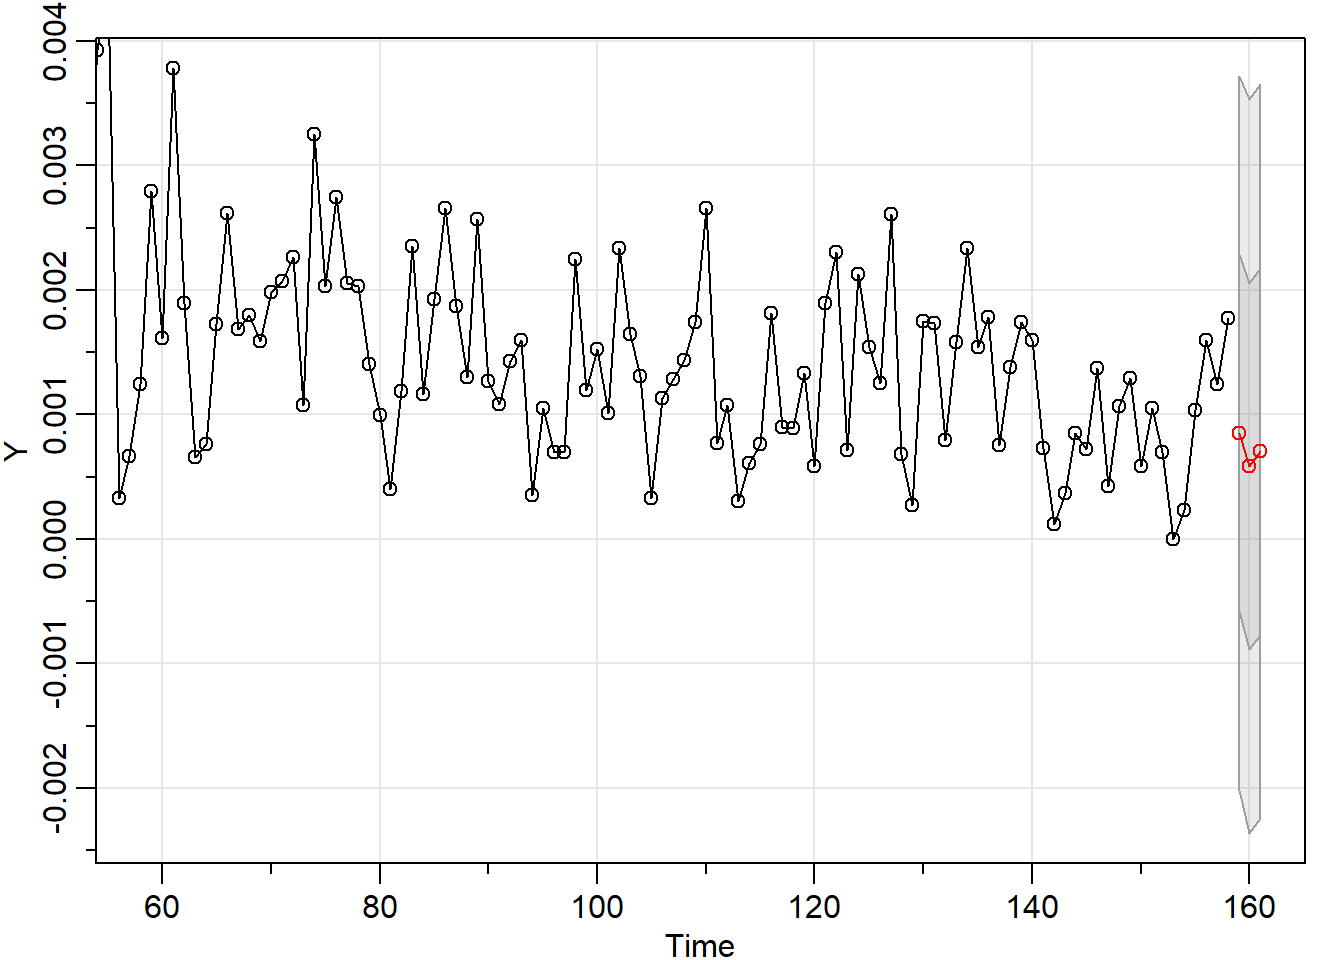
\includegraphics{03_EJERCICIOS_files/figure-latex/unnamed-chunk-2-3.pdf} 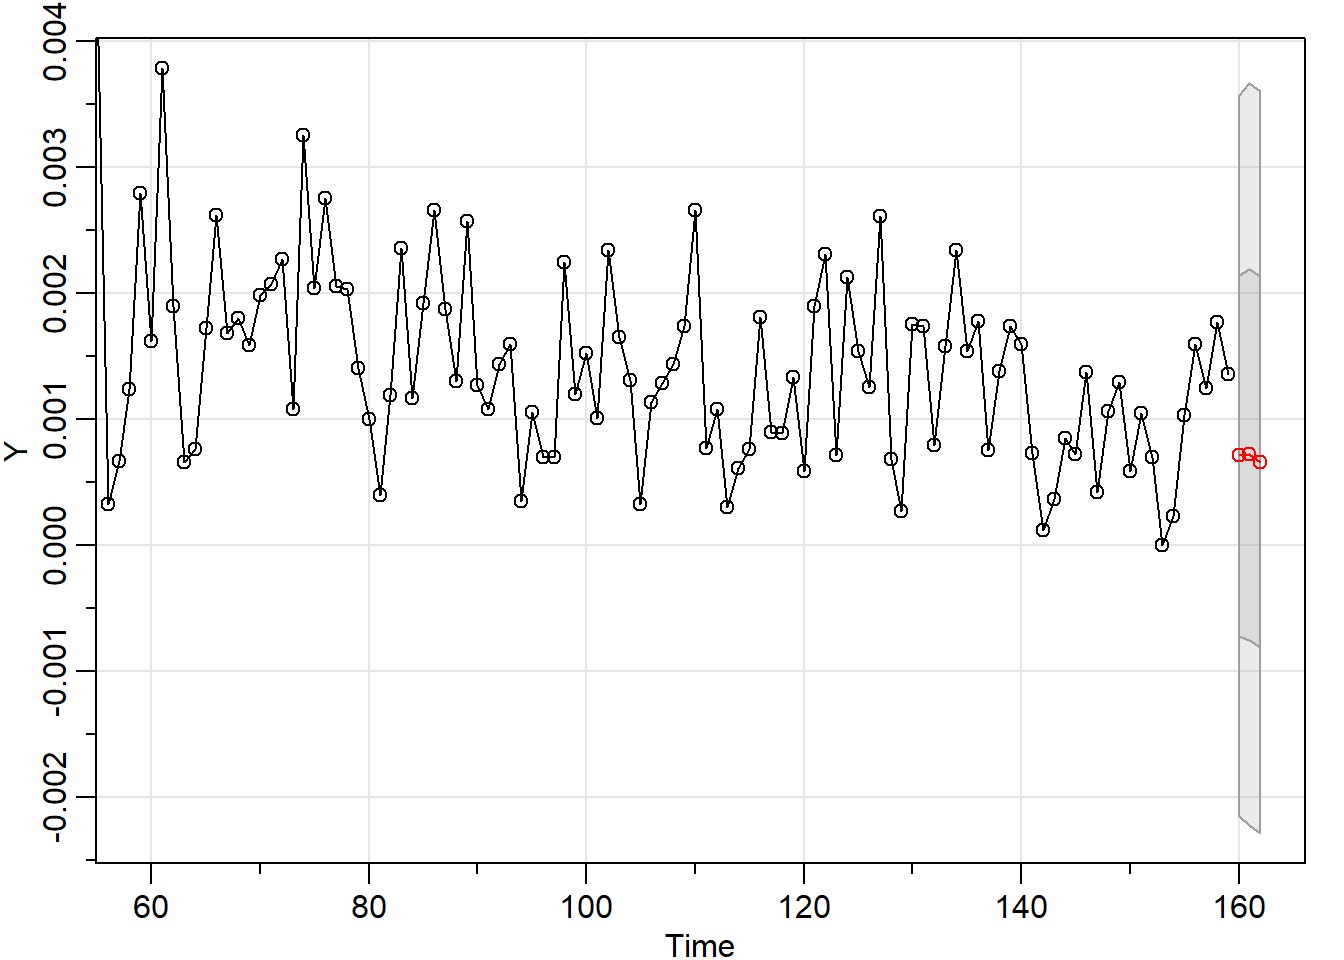
\includegraphics{03_EJERCICIOS_files/figure-latex/unnamed-chunk-2-4.pdf} 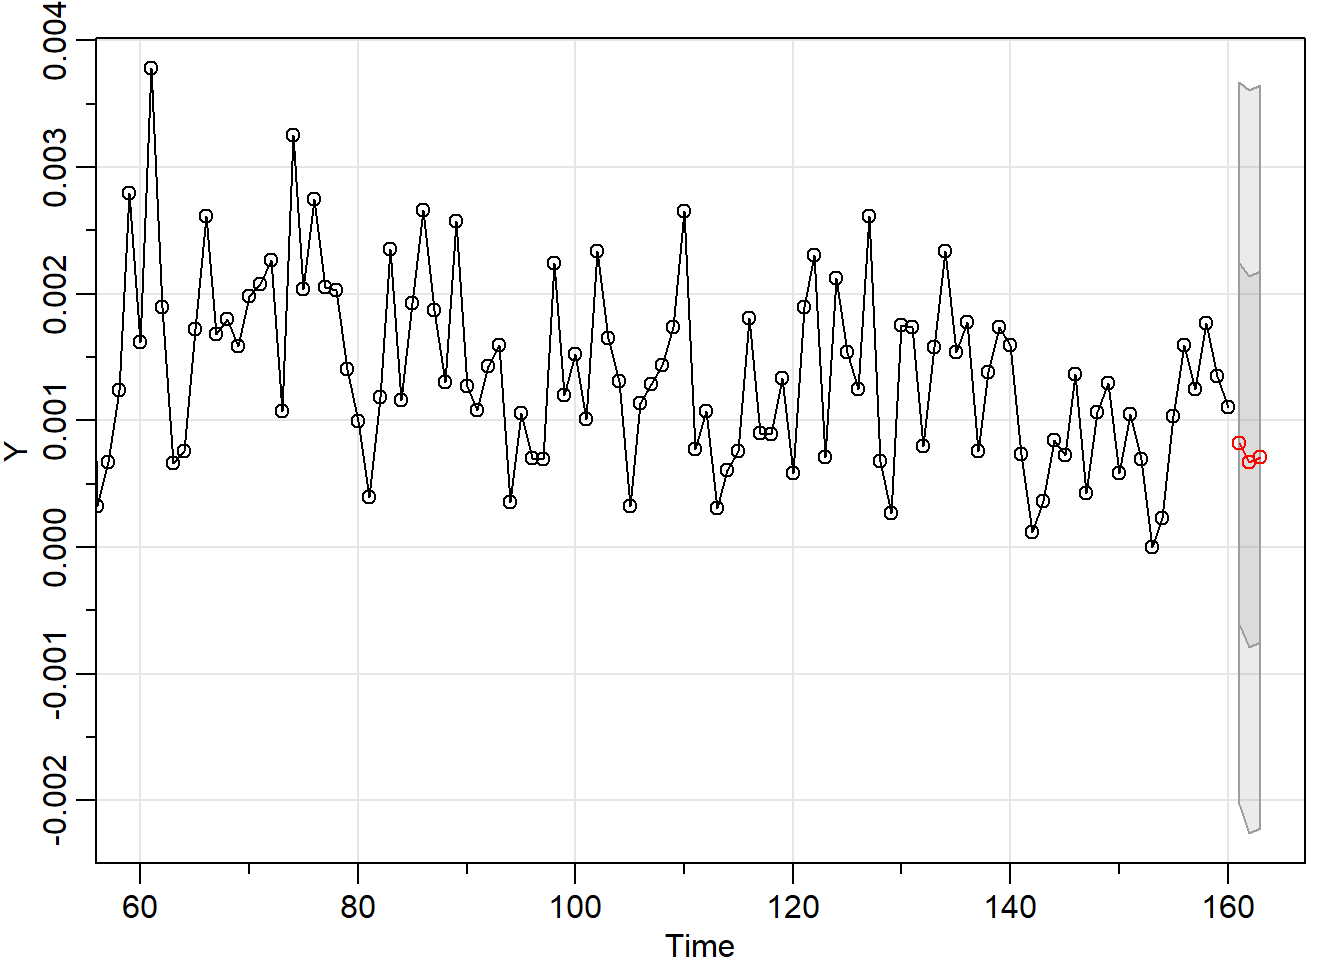
\includegraphics{03_EJERCICIOS_files/figure-latex/unnamed-chunk-2-5.pdf} 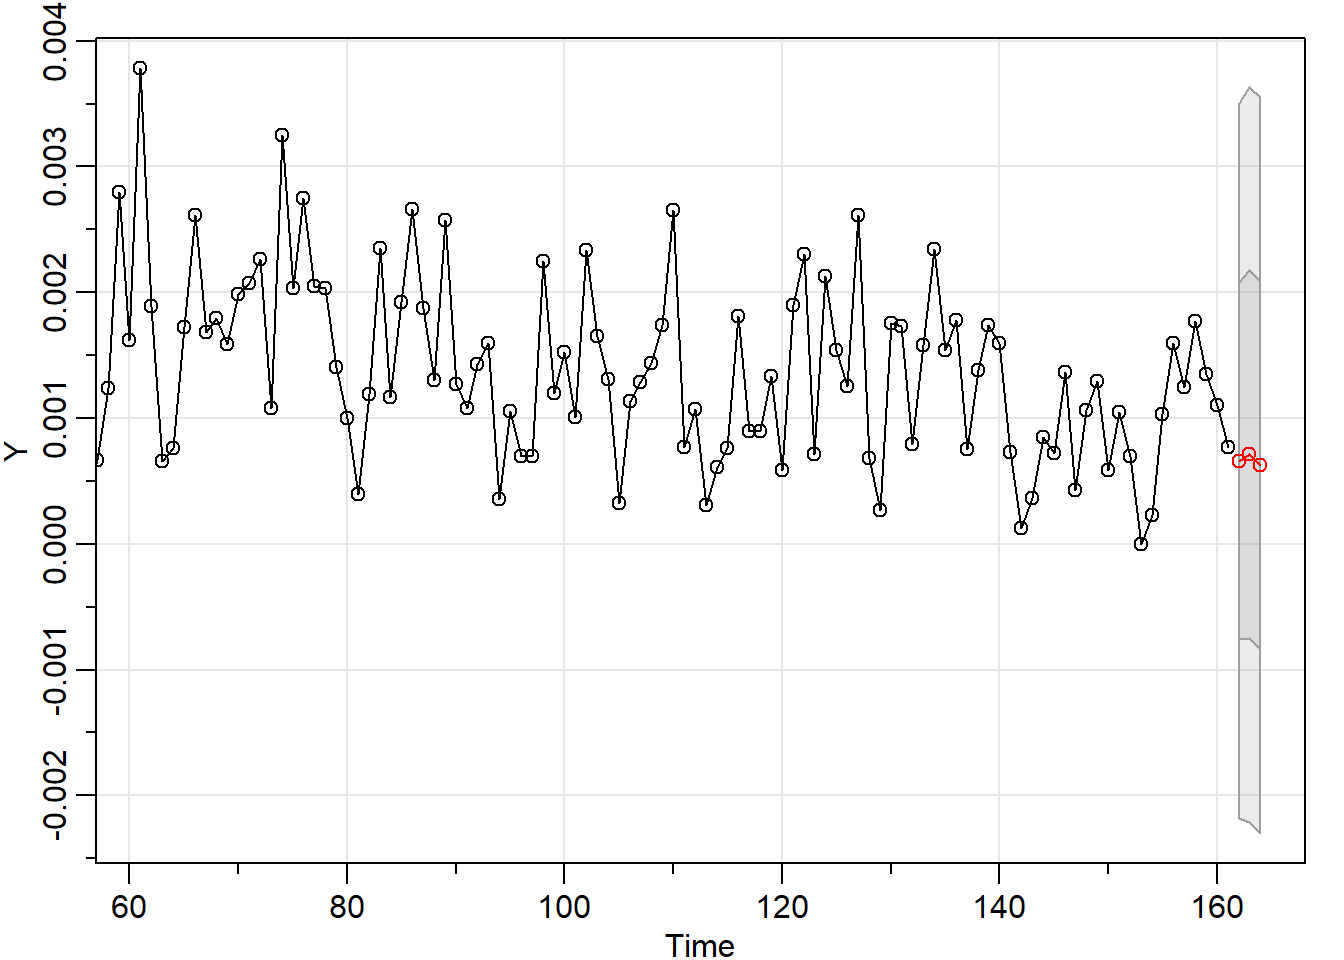
\includegraphics{03_EJERCICIOS_files/figure-latex/unnamed-chunk-2-6.pdf} 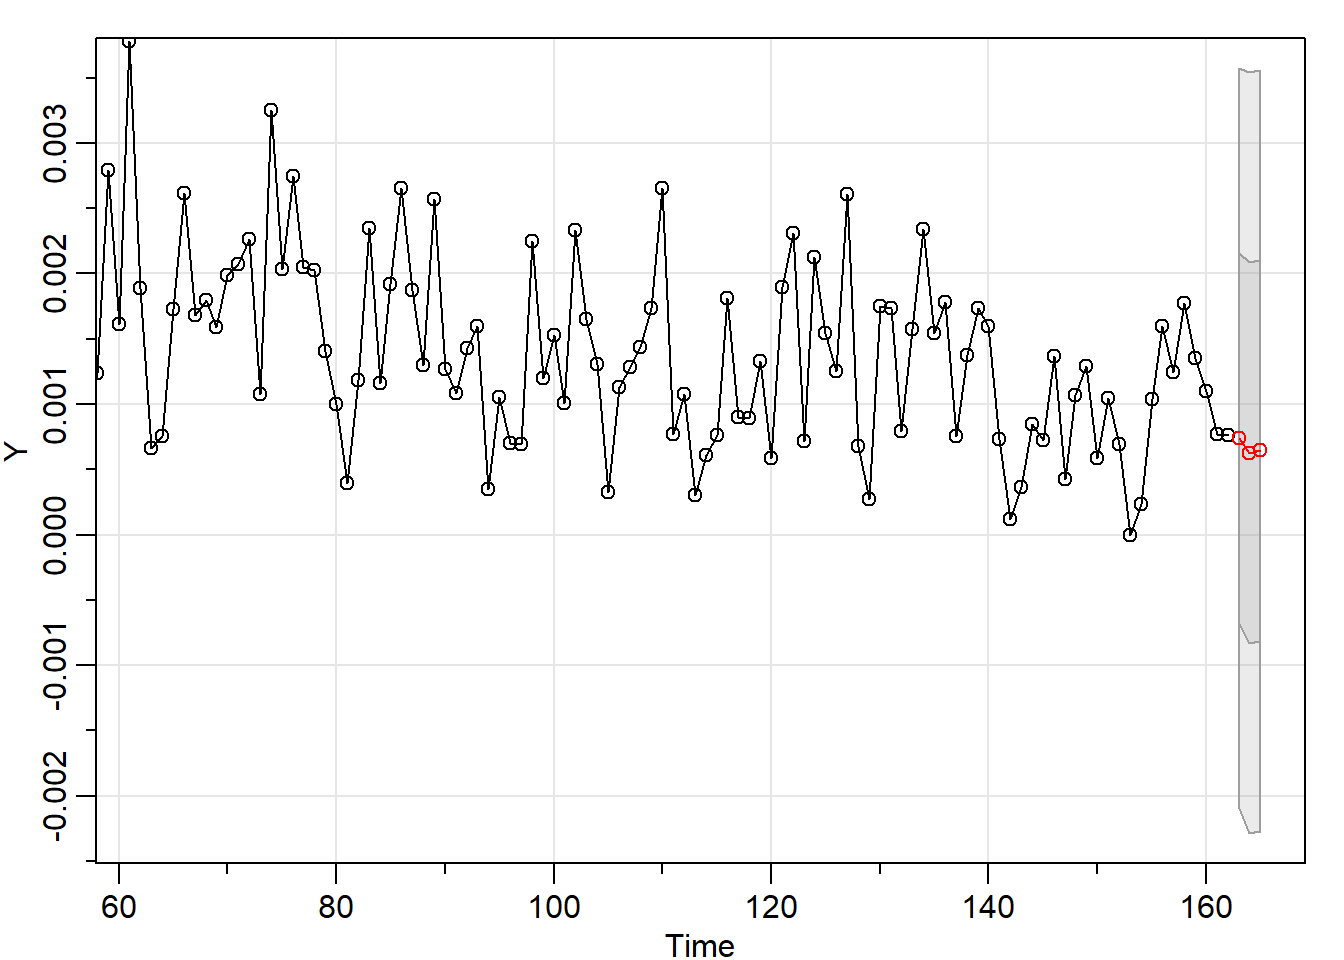
\includegraphics{03_EJERCICIOS_files/figure-latex/unnamed-chunk-2-7.pdf} 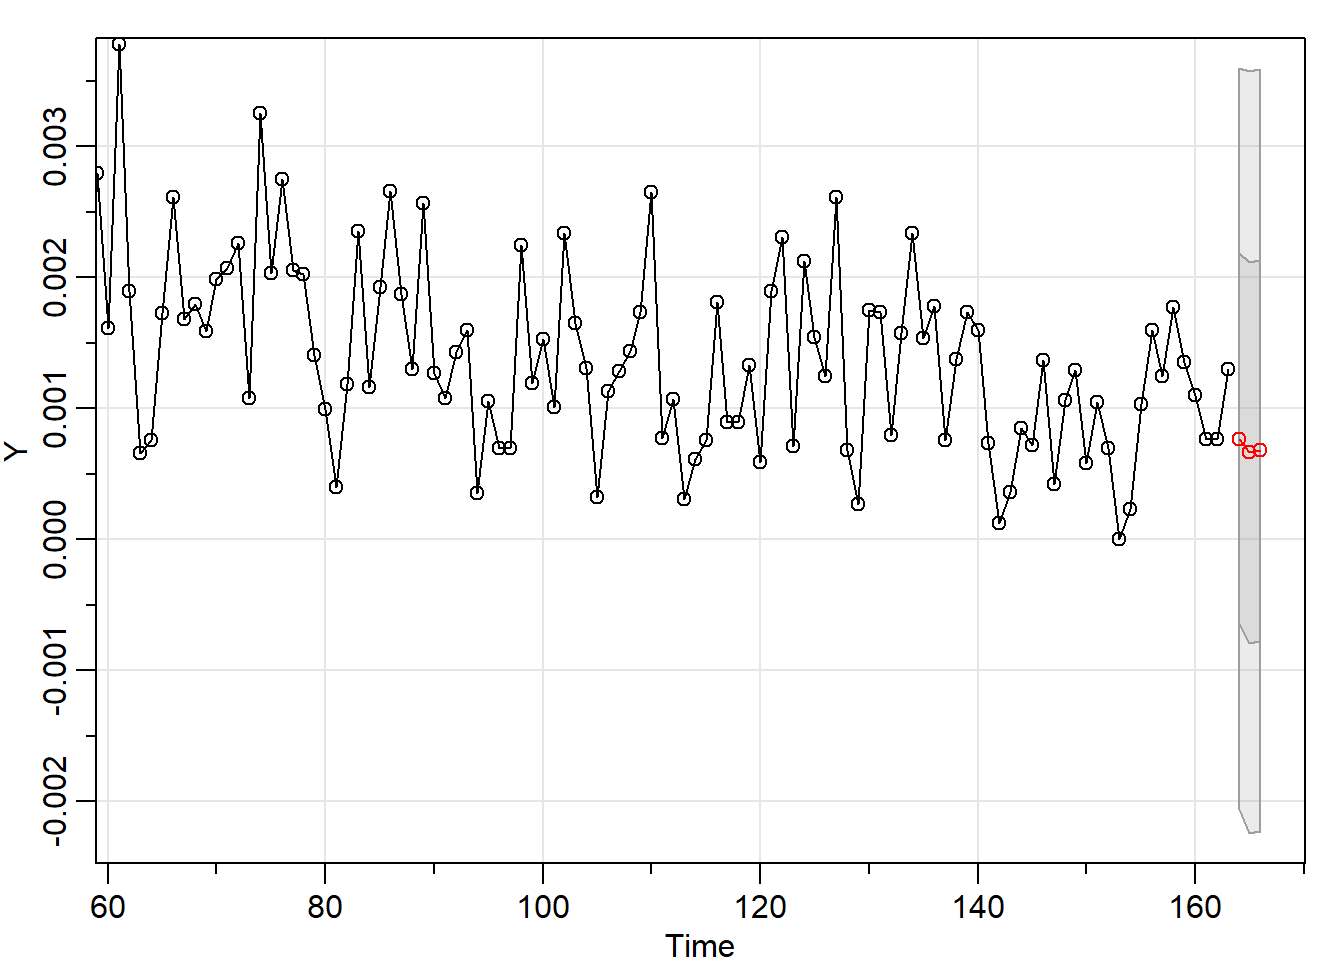
\includegraphics{03_EJERCICIOS_files/figure-latex/unnamed-chunk-2-8.pdf} 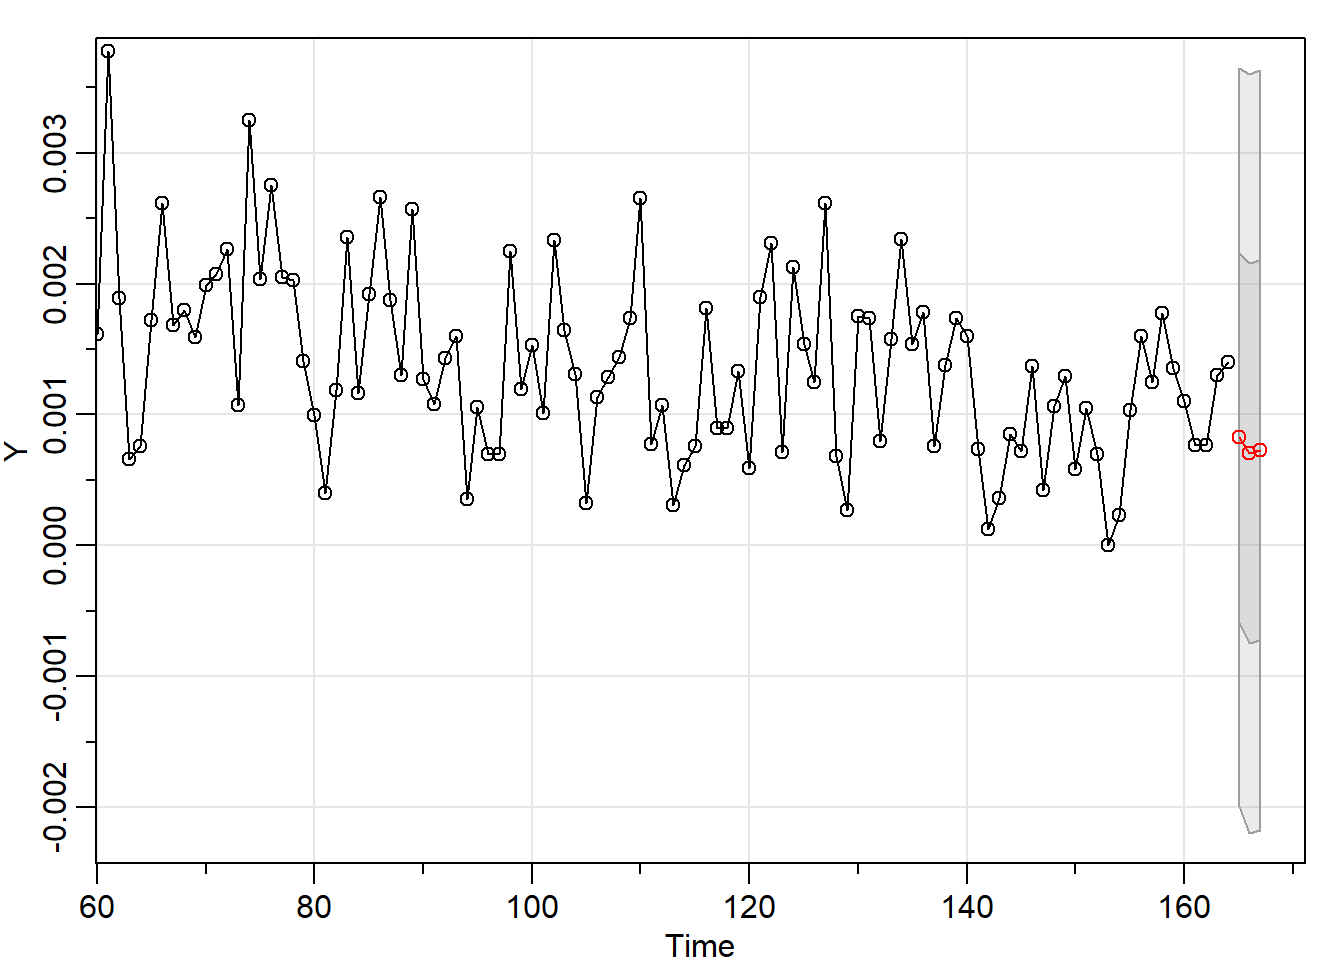
\includegraphics{03_EJERCICIOS_files/figure-latex/unnamed-chunk-2-9.pdf} 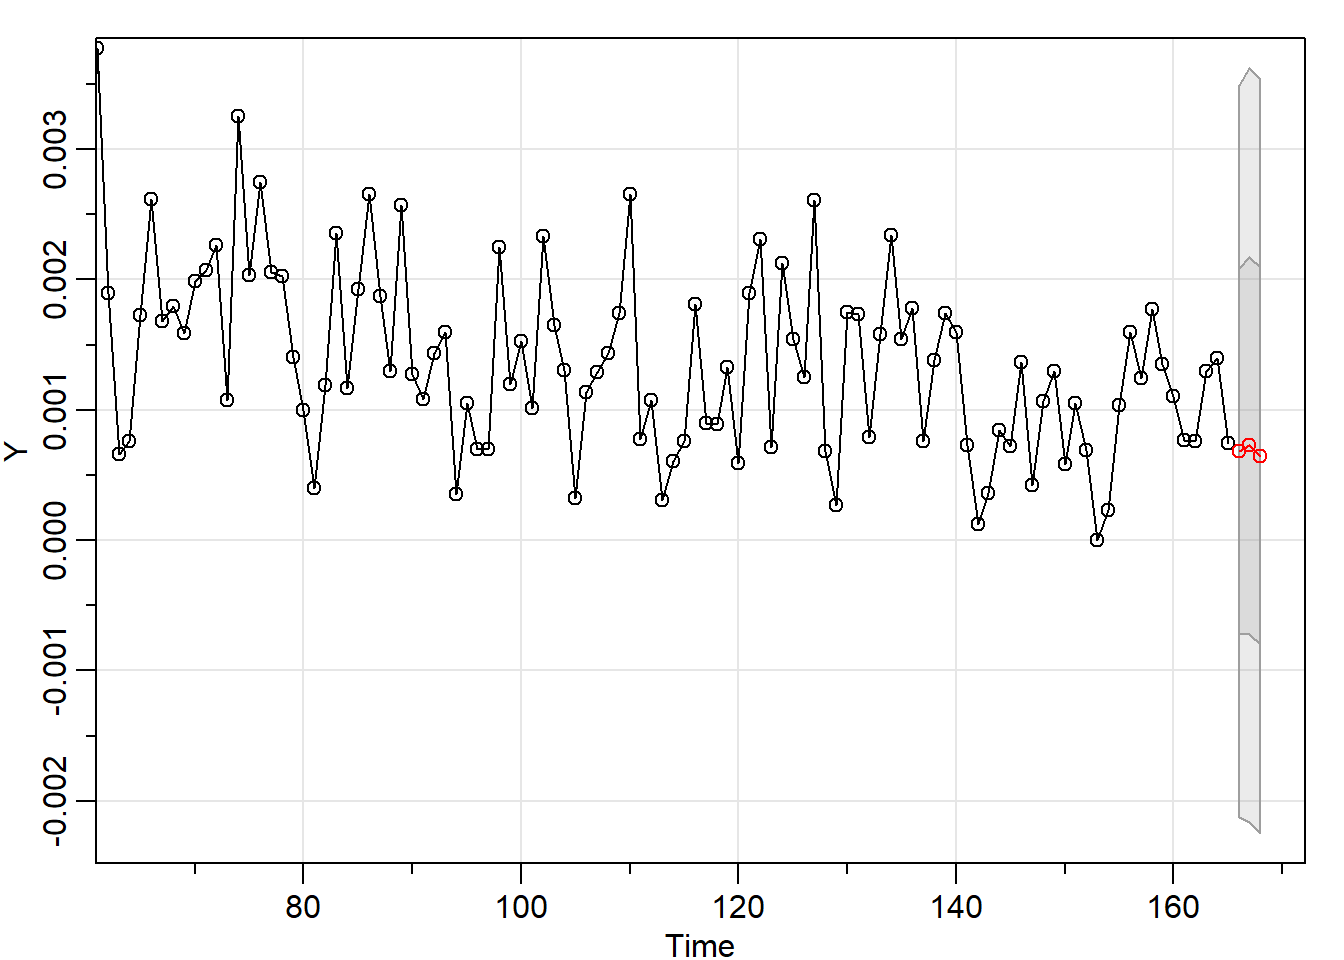
\includegraphics{03_EJERCICIOS_files/figure-latex/unnamed-chunk-2-10.pdf} 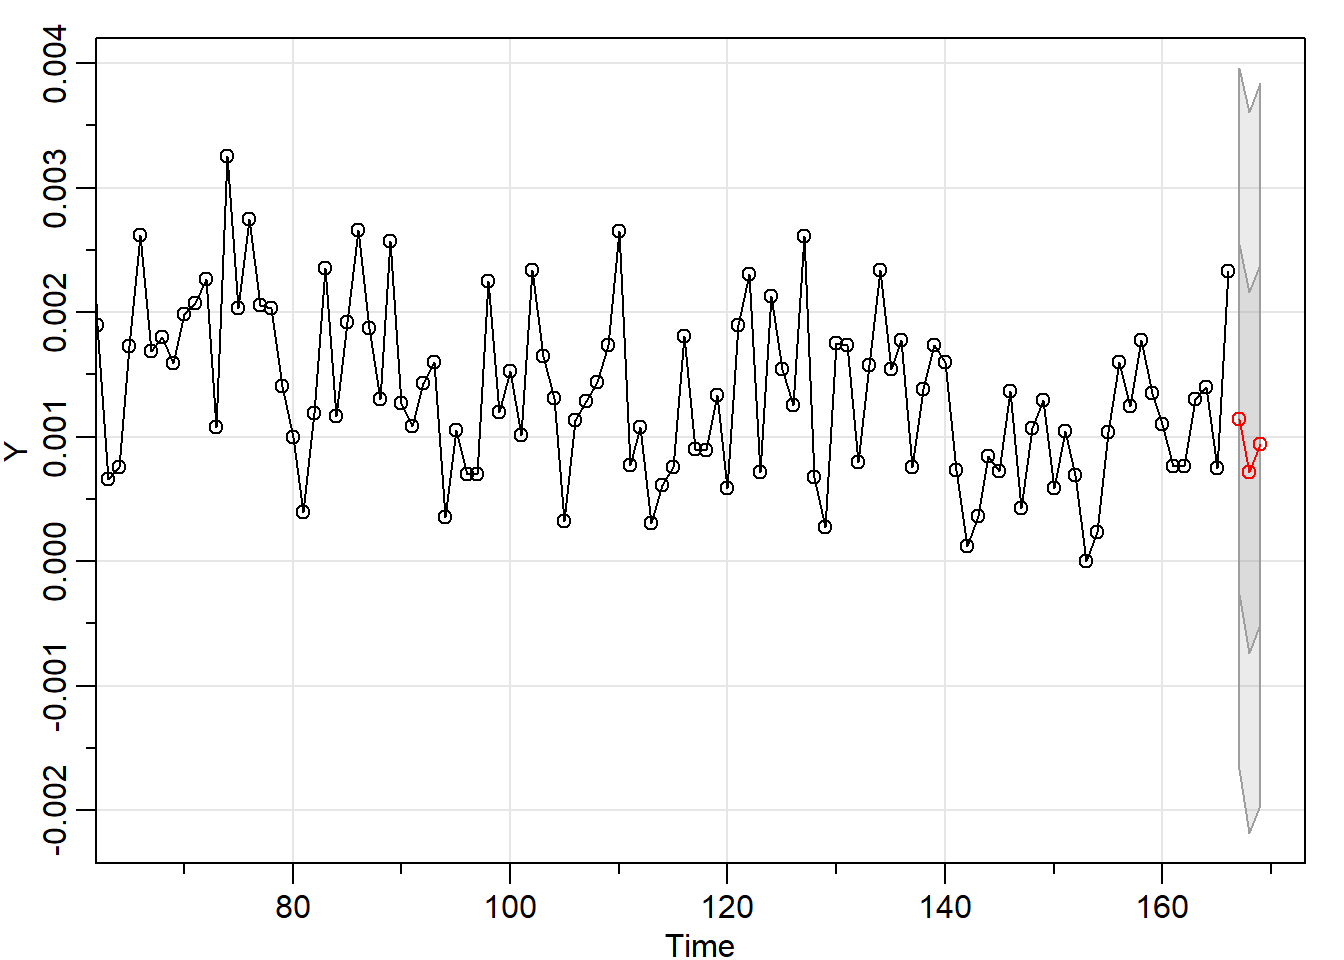
\includegraphics{03_EJERCICIOS_files/figure-latex/unnamed-chunk-2-11.pdf} 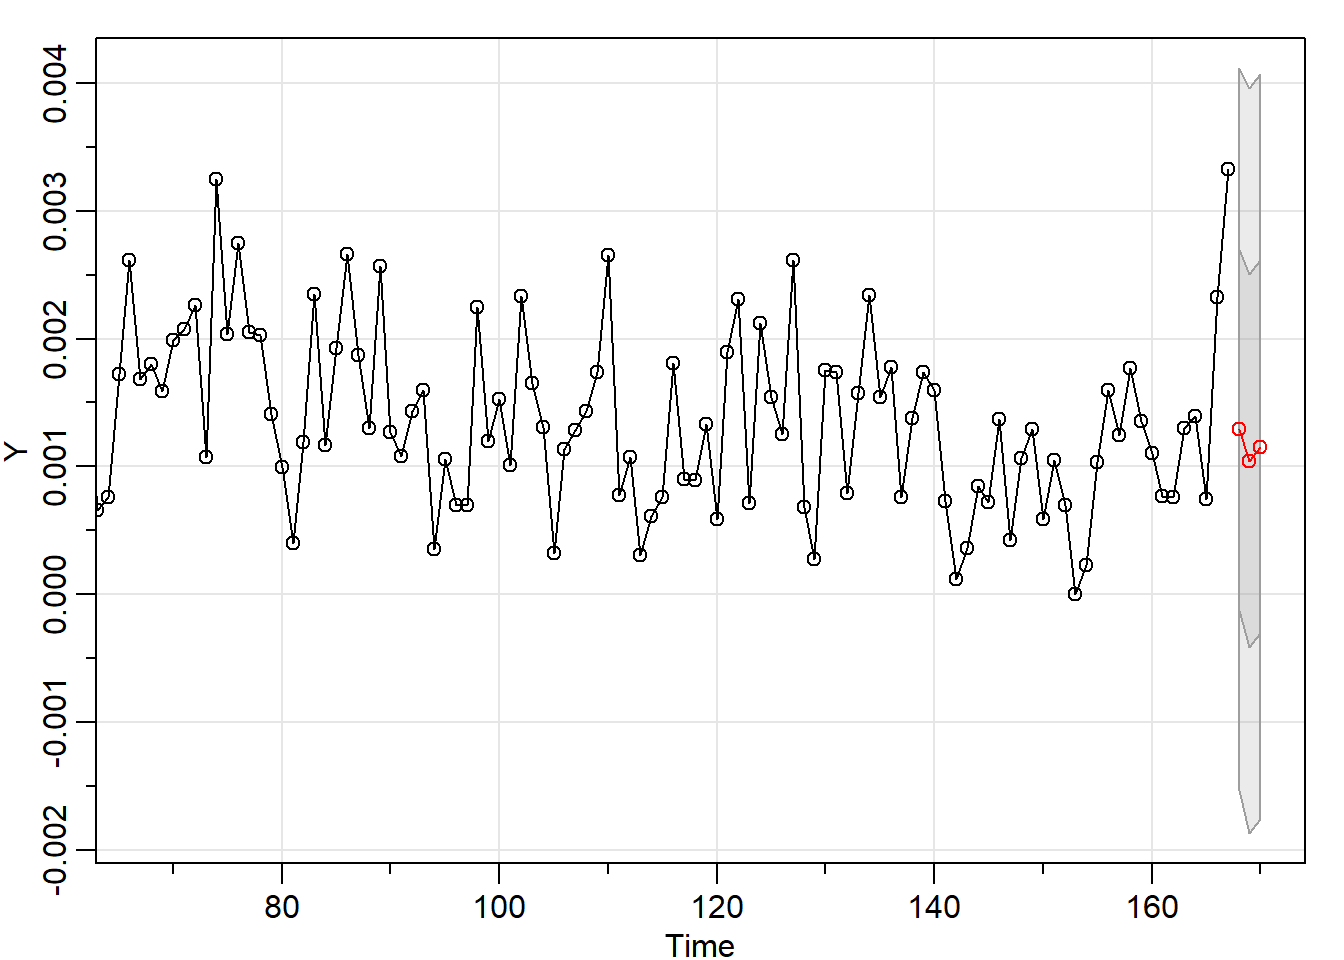
\includegraphics{03_EJERCICIOS_files/figure-latex/unnamed-chunk-2-12.pdf} 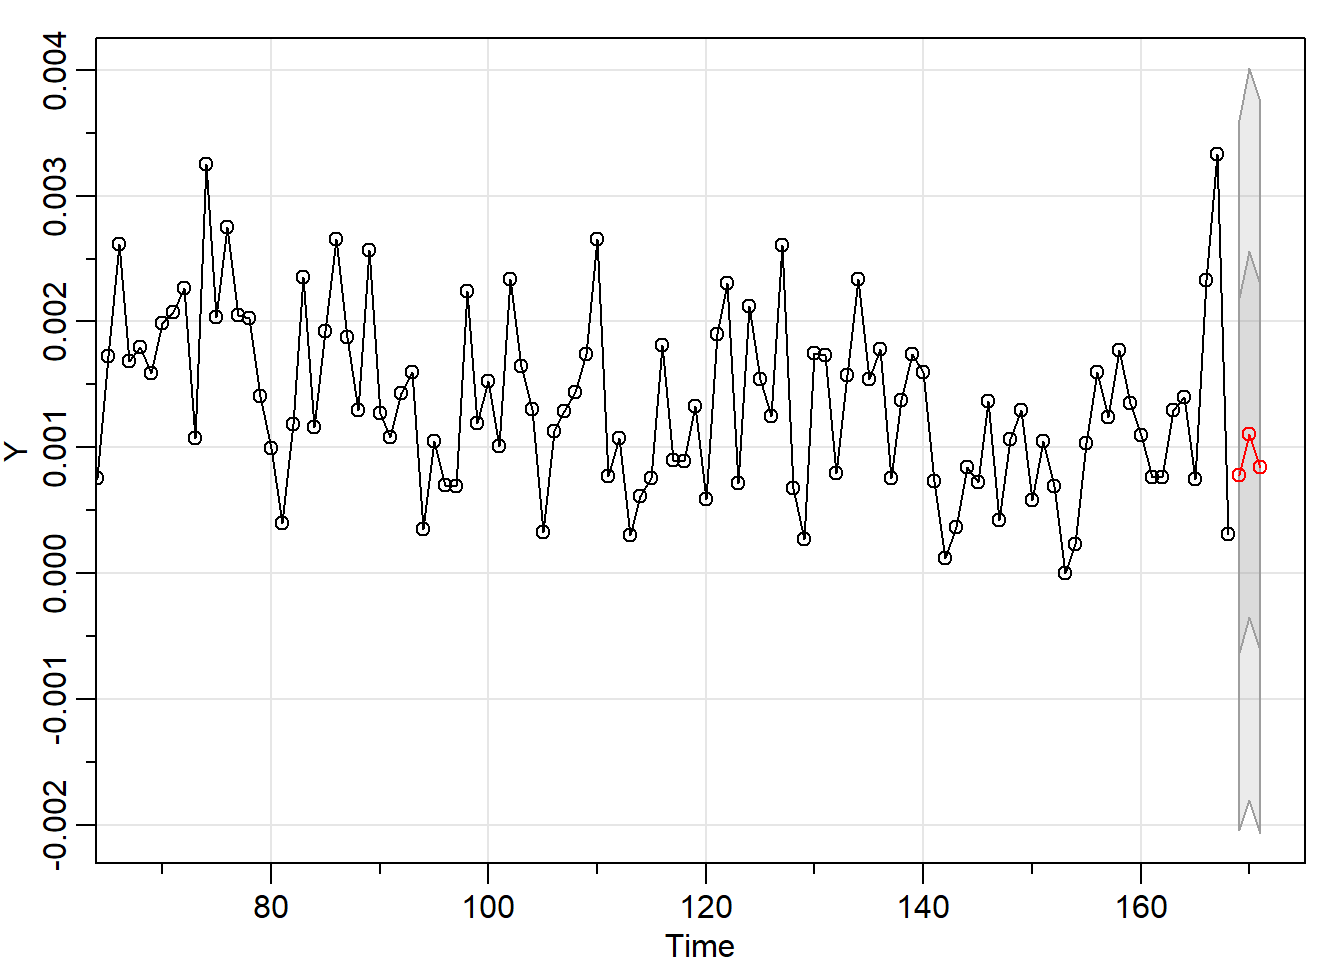
\includegraphics{03_EJERCICIOS_files/figure-latex/unnamed-chunk-2-13.pdf} 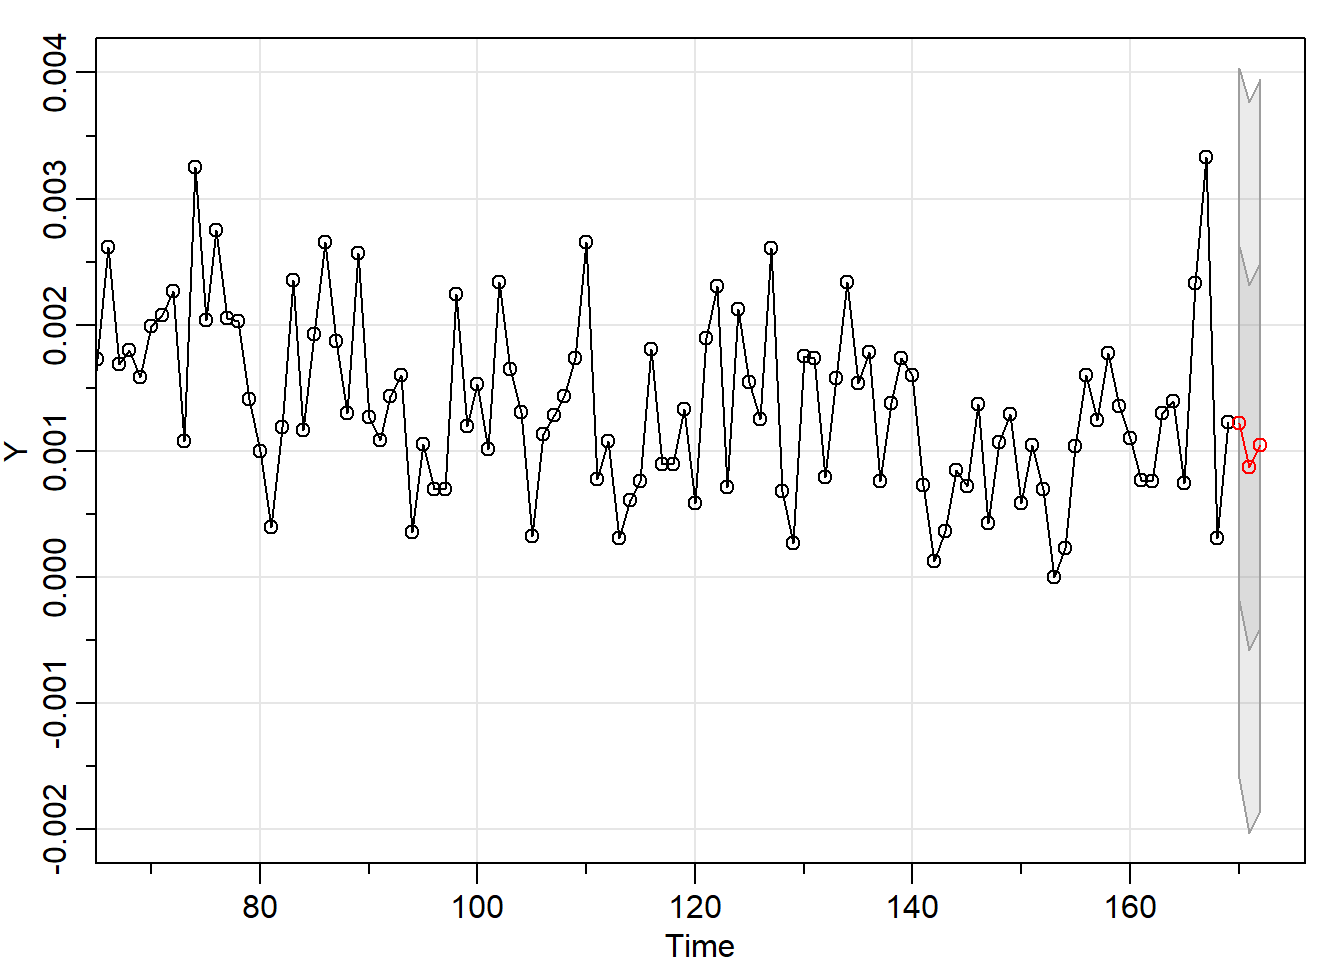
\includegraphics{03_EJERCICIOS_files/figure-latex/unnamed-chunk-2-14.pdf} 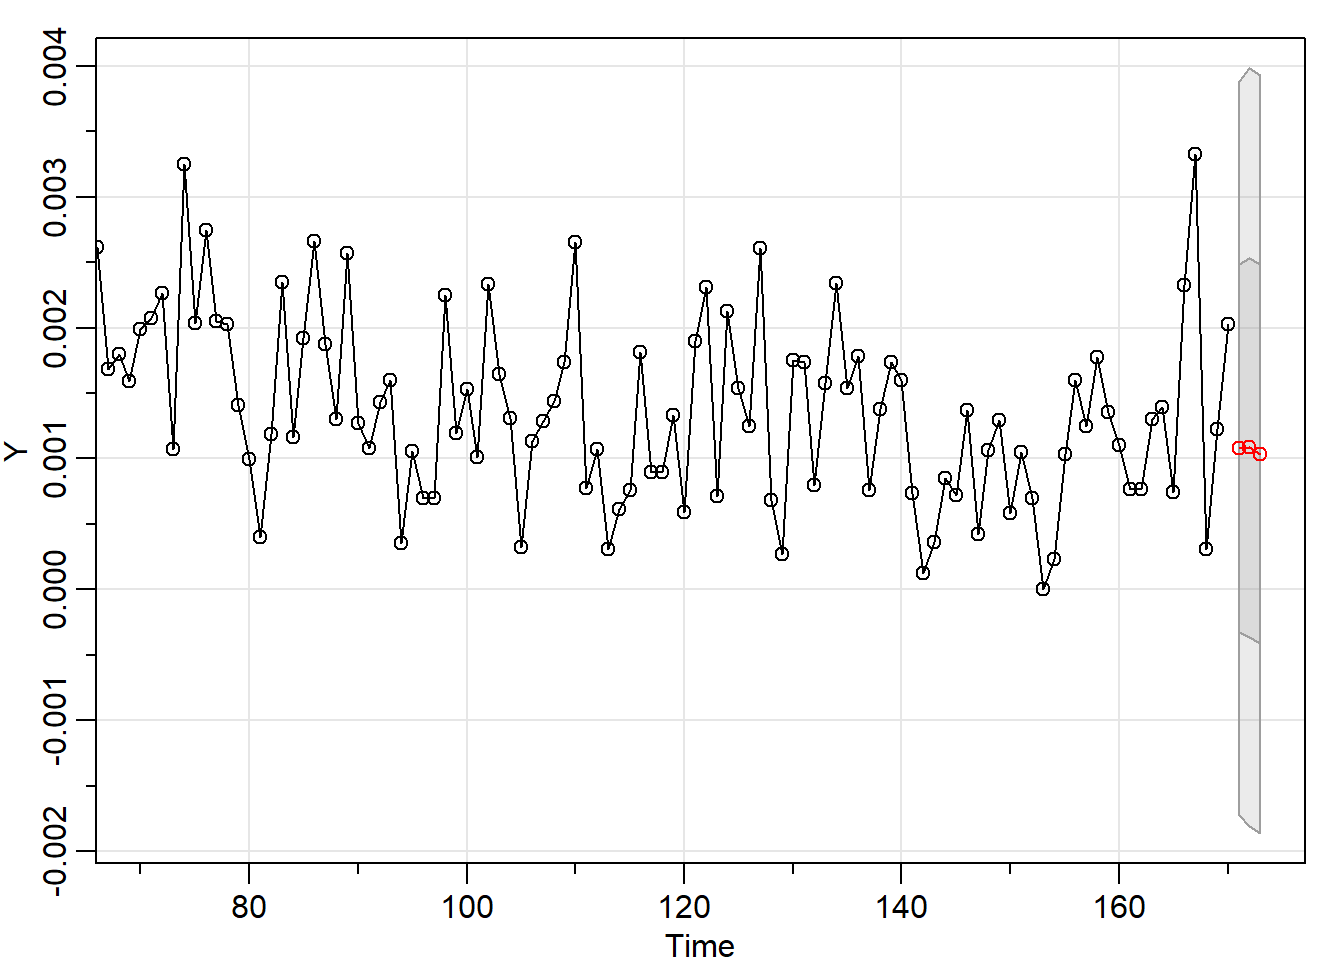
\includegraphics{03_EJERCICIOS_files/figure-latex/unnamed-chunk-2-15.pdf} 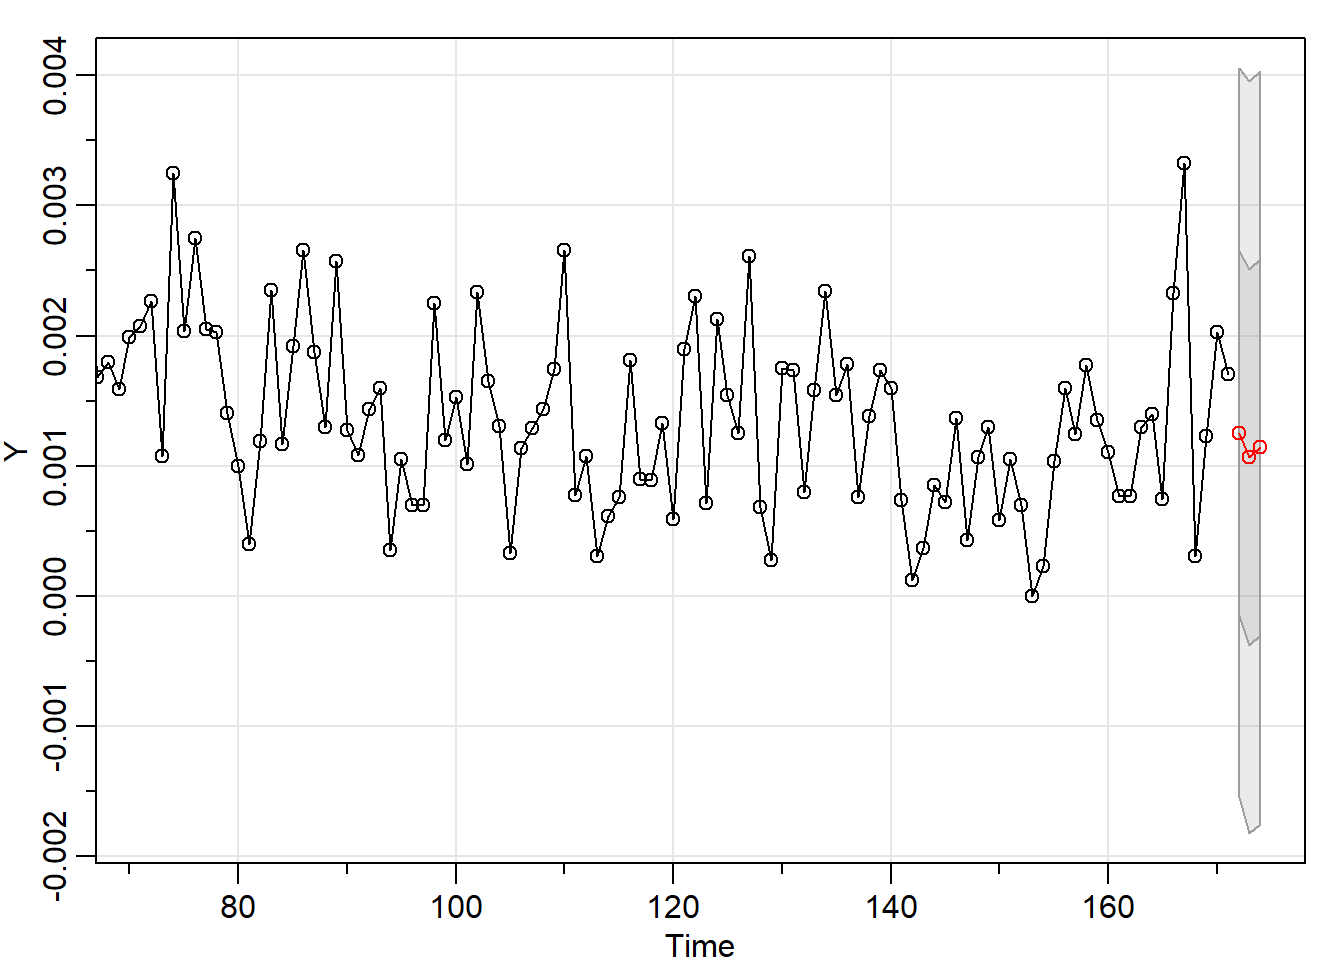
\includegraphics{03_EJERCICIOS_files/figure-latex/unnamed-chunk-2-16.pdf} 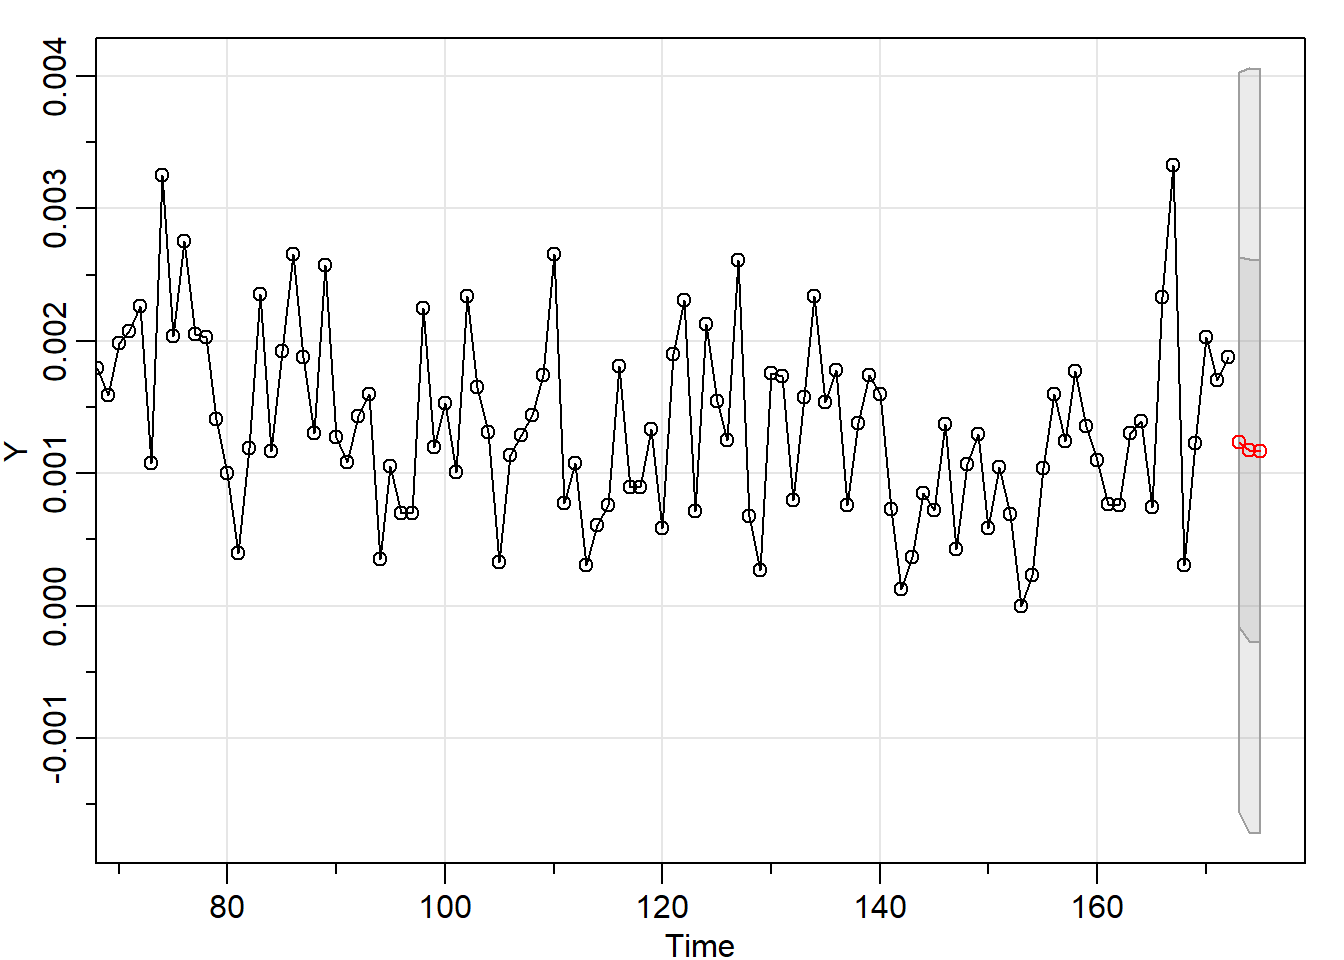
\includegraphics{03_EJERCICIOS_files/figure-latex/unnamed-chunk-2-17.pdf} 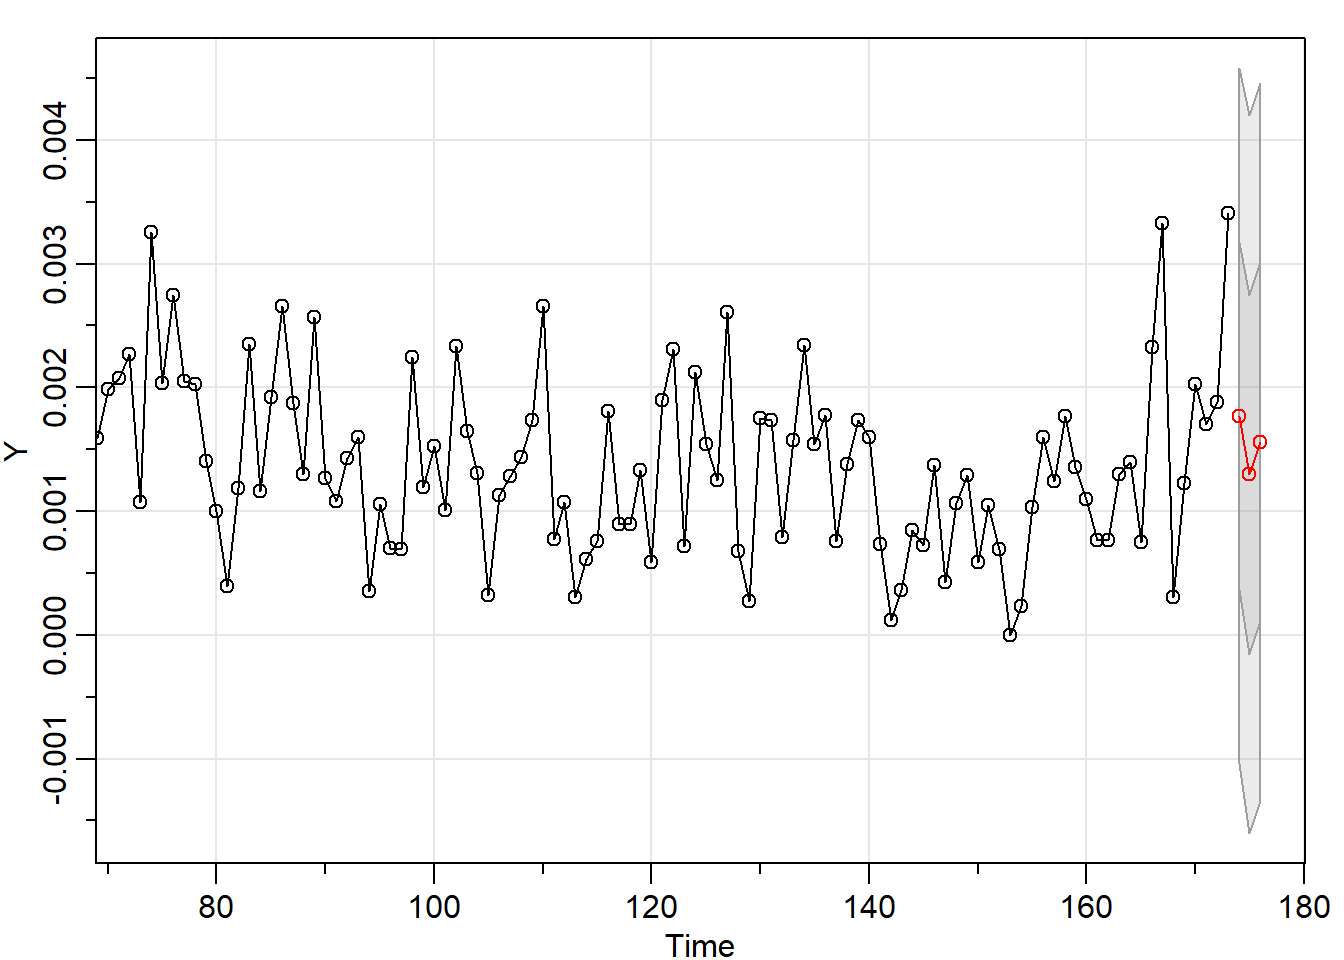
\includegraphics{03_EJERCICIOS_files/figure-latex/unnamed-chunk-2-18.pdf} 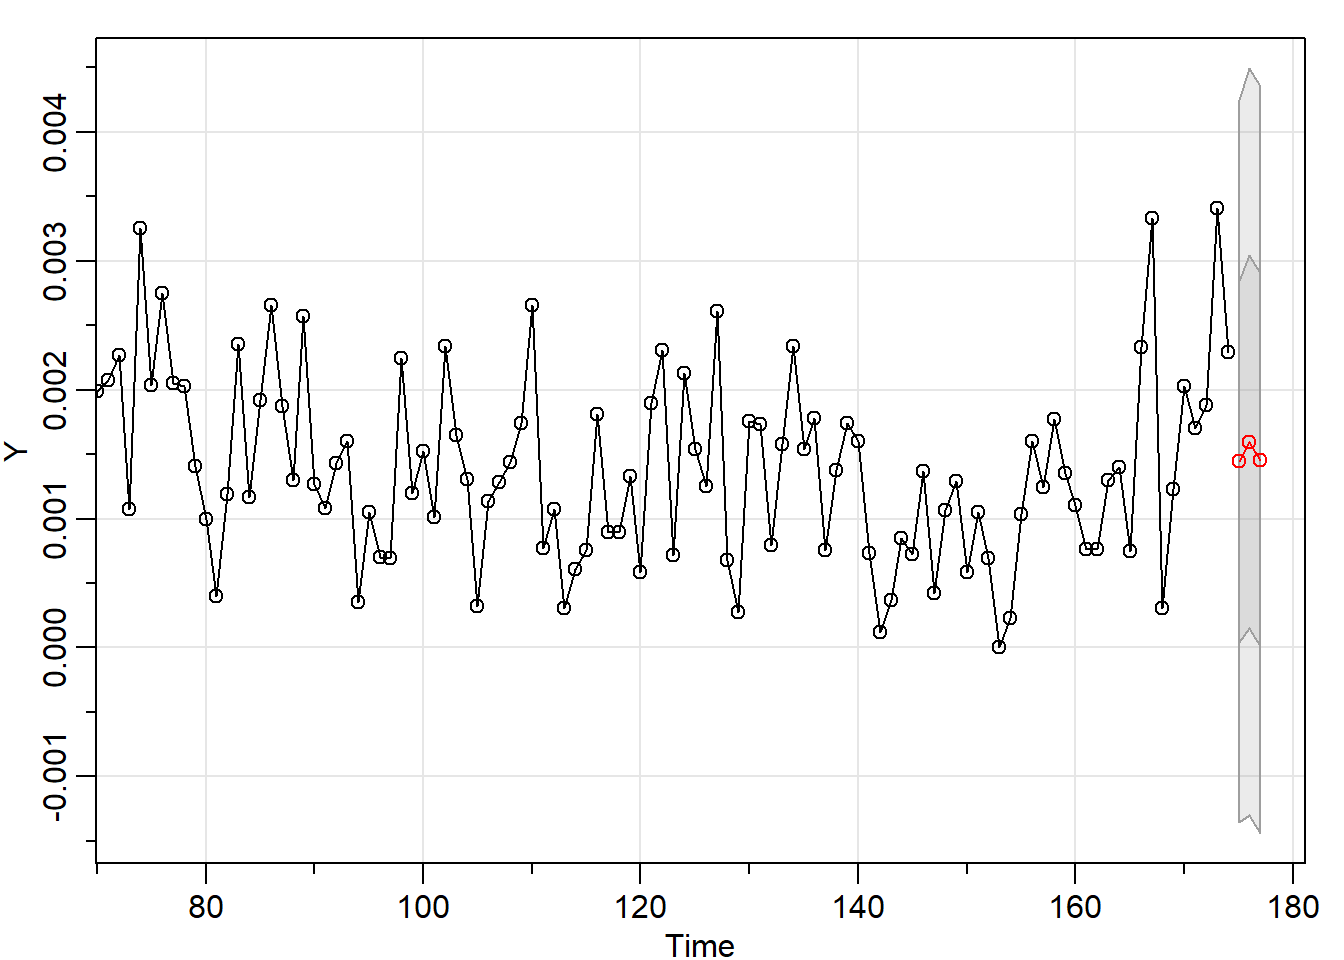
\includegraphics{03_EJERCICIOS_files/figure-latex/unnamed-chunk-2-19.pdf} 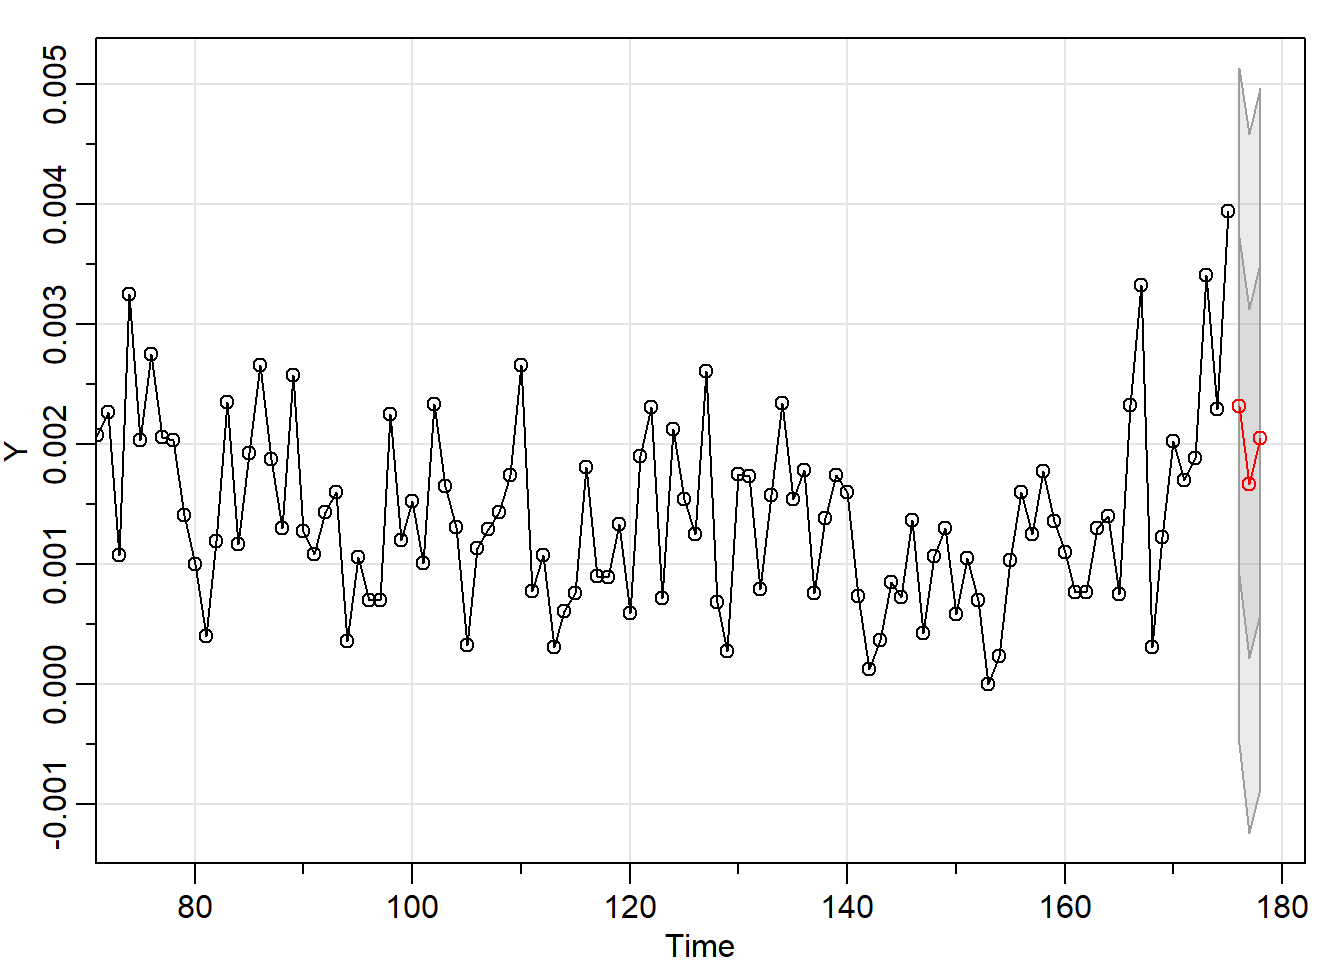
\includegraphics{03_EJERCICIOS_files/figure-latex/unnamed-chunk-2-20.pdf} 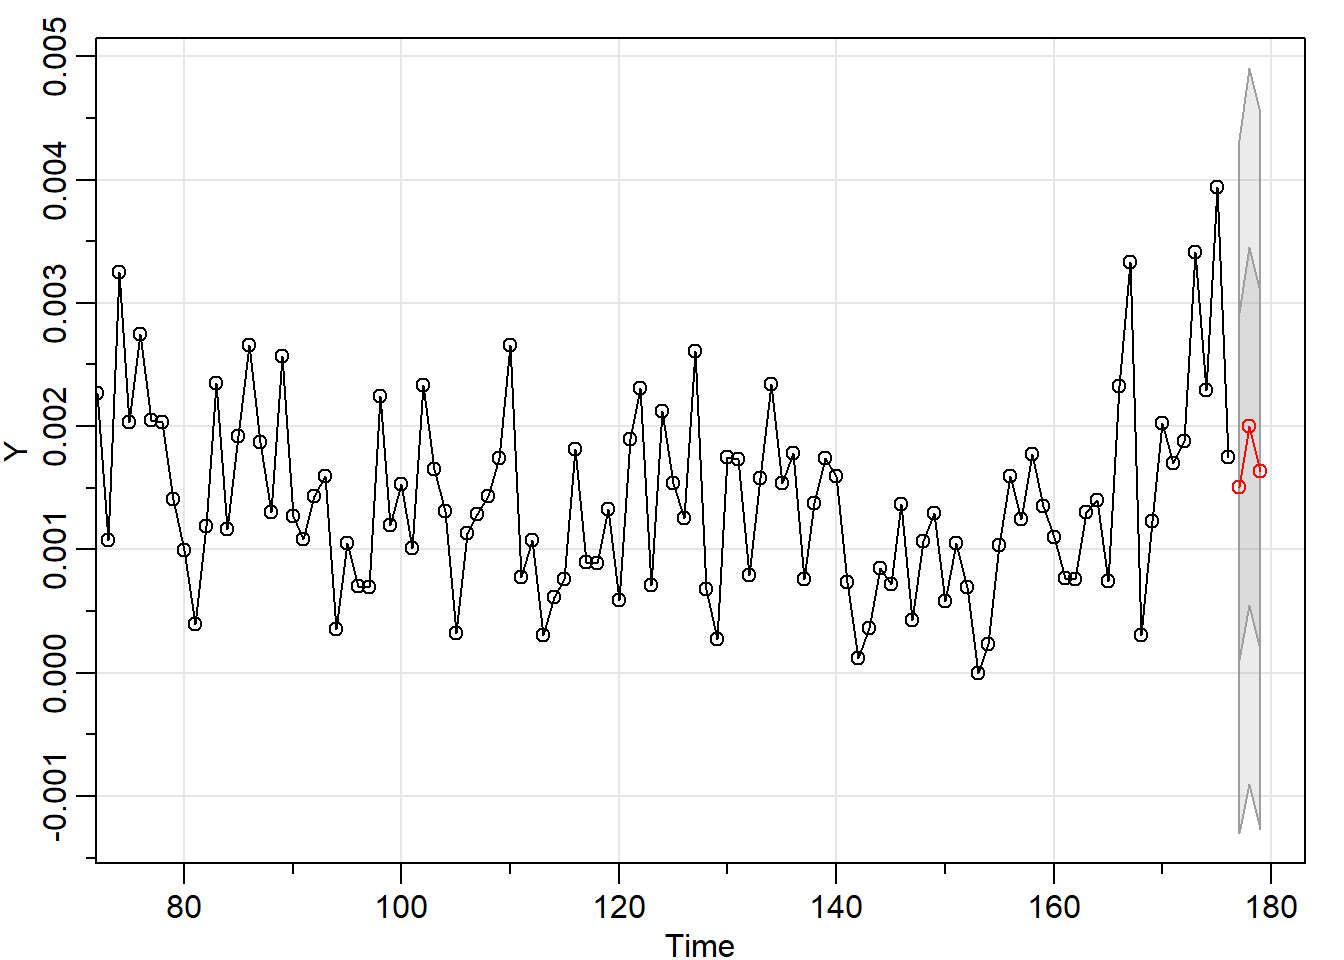
\includegraphics{03_EJERCICIOS_files/figure-latex/unnamed-chunk-2-21.pdf} 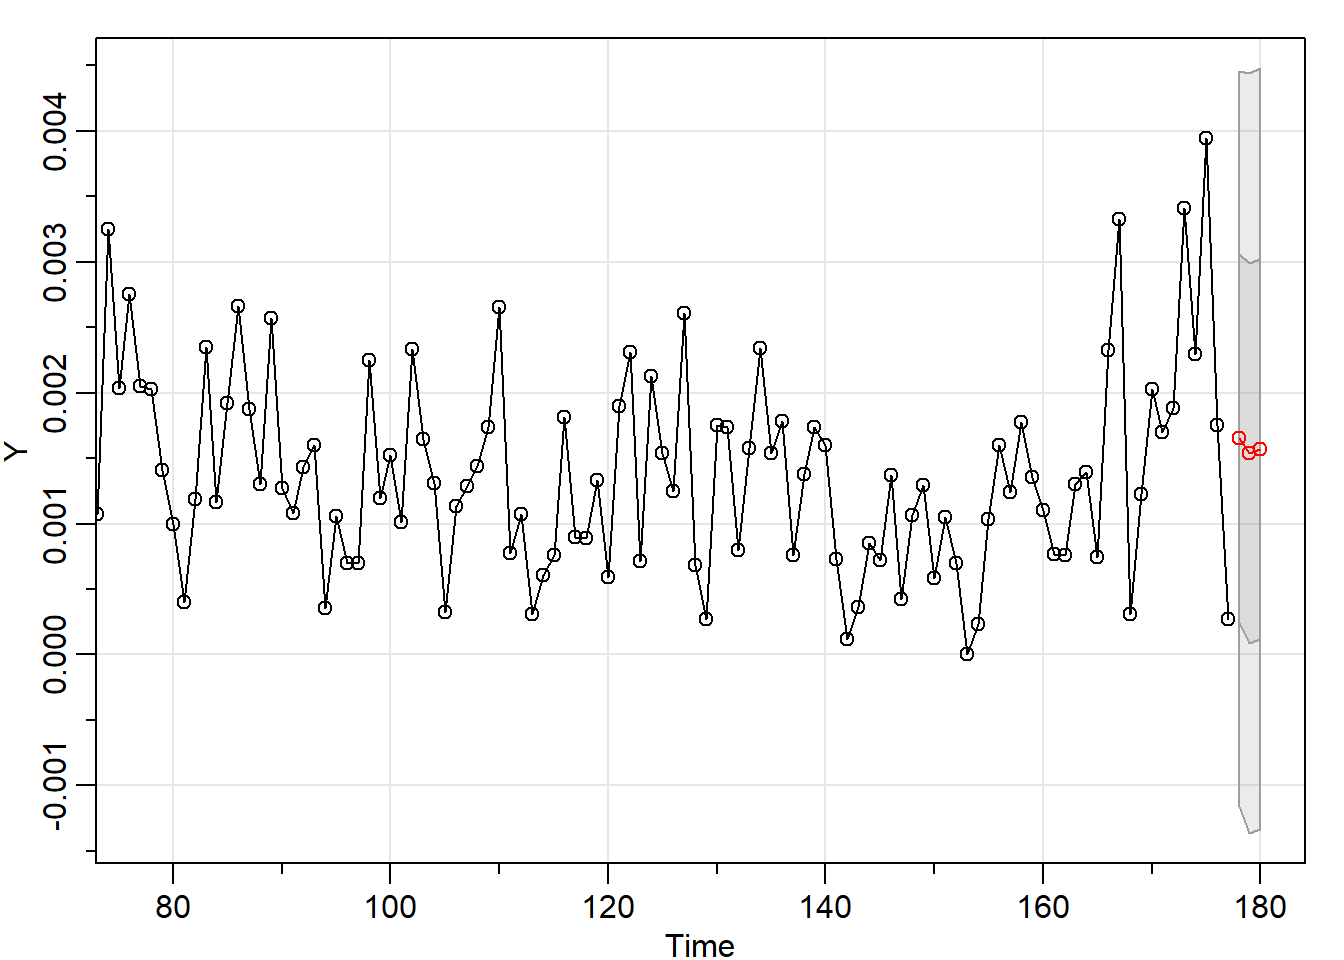
\includegraphics{03_EJERCICIOS_files/figure-latex/unnamed-chunk-2-22.pdf} \includegraphics{03_EJERCICIOS_files/figure-latex/unnamed-chunk-2-23.pdf} \includegraphics{03_EJERCICIOS_files/figure-latex/unnamed-chunk-2-24.pdf} \includegraphics{03_EJERCICIOS_files/figure-latex/unnamed-chunk-2-25.pdf} \includegraphics{03_EJERCICIOS_files/figure-latex/unnamed-chunk-2-26.pdf} \includegraphics{03_EJERCICIOS_files/figure-latex/unnamed-chunk-2-27.pdf} \includegraphics{03_EJERCICIOS_files/figure-latex/unnamed-chunk-2-28.pdf} \includegraphics{03_EJERCICIOS_files/figure-latex/unnamed-chunk-2-29.pdf} \includegraphics{03_EJERCICIOS_files/figure-latex/unnamed-chunk-2-30.pdf} \includegraphics{03_EJERCICIOS_files/figure-latex/unnamed-chunk-2-31.pdf} \includegraphics{03_EJERCICIOS_files/figure-latex/unnamed-chunk-2-32.pdf} \includegraphics{03_EJERCICIOS_files/figure-latex/unnamed-chunk-2-33.pdf} \includegraphics{03_EJERCICIOS_files/figure-latex/unnamed-chunk-2-34.pdf} \includegraphics{03_EJERCICIOS_files/figure-latex/unnamed-chunk-2-35.pdf} \includegraphics{03_EJERCICIOS_files/figure-latex/unnamed-chunk-2-36.pdf} \includegraphics{03_EJERCICIOS_files/figure-latex/unnamed-chunk-2-37.pdf} \includegraphics{03_EJERCICIOS_files/figure-latex/unnamed-chunk-2-38.pdf} \includegraphics{03_EJERCICIOS_files/figure-latex/unnamed-chunk-2-39.pdf} \includegraphics{03_EJERCICIOS_files/figure-latex/unnamed-chunk-2-40.pdf} \includegraphics{03_EJERCICIOS_files/figure-latex/unnamed-chunk-2-41.pdf} \includegraphics{03_EJERCICIOS_files/figure-latex/unnamed-chunk-2-42.pdf} \includegraphics{03_EJERCICIOS_files/figure-latex/unnamed-chunk-2-43.pdf} \includegraphics{03_EJERCICIOS_files/figure-latex/unnamed-chunk-2-44.pdf} \includegraphics{03_EJERCICIOS_files/figure-latex/unnamed-chunk-2-45.pdf} \includegraphics{03_EJERCICIOS_files/figure-latex/unnamed-chunk-2-46.pdf} \includegraphics{03_EJERCICIOS_files/figure-latex/unnamed-chunk-2-47.pdf} \includegraphics{03_EJERCICIOS_files/figure-latex/unnamed-chunk-2-48.pdf} \includegraphics{03_EJERCICIOS_files/figure-latex/unnamed-chunk-2-49.pdf} \includegraphics{03_EJERCICIOS_files/figure-latex/unnamed-chunk-2-50.pdf} \includegraphics{03_EJERCICIOS_files/figure-latex/unnamed-chunk-2-51.pdf} \includegraphics{03_EJERCICIOS_files/figure-latex/unnamed-chunk-2-52.pdf} \includegraphics{03_EJERCICIOS_files/figure-latex/unnamed-chunk-2-53.pdf} \includegraphics{03_EJERCICIOS_files/figure-latex/unnamed-chunk-2-54.pdf} \includegraphics{03_EJERCICIOS_files/figure-latex/unnamed-chunk-2-55.pdf} \includegraphics{03_EJERCICIOS_files/figure-latex/unnamed-chunk-2-56.pdf} \includegraphics{03_EJERCICIOS_files/figure-latex/unnamed-chunk-2-57.pdf} \includegraphics{03_EJERCICIOS_files/figure-latex/unnamed-chunk-2-58.pdf} \includegraphics{03_EJERCICIOS_files/figure-latex/unnamed-chunk-2-59.pdf} \includegraphics{03_EJERCICIOS_files/figure-latex/unnamed-chunk-2-60.pdf} \includegraphics{03_EJERCICIOS_files/figure-latex/unnamed-chunk-2-61.pdf} \includegraphics{03_EJERCICIOS_files/figure-latex/unnamed-chunk-2-62.pdf} \includegraphics{03_EJERCICIOS_files/figure-latex/unnamed-chunk-2-63.pdf} \includegraphics{03_EJERCICIOS_files/figure-latex/unnamed-chunk-2-64.pdf} \includegraphics{03_EJERCICIOS_files/figure-latex/unnamed-chunk-2-65.pdf} \includegraphics{03_EJERCICIOS_files/figure-latex/unnamed-chunk-2-66.pdf} \includegraphics{03_EJERCICIOS_files/figure-latex/unnamed-chunk-2-67.pdf} \includegraphics{03_EJERCICIOS_files/figure-latex/unnamed-chunk-2-68.pdf} \includegraphics{03_EJERCICIOS_files/figure-latex/unnamed-chunk-2-69.pdf} \includegraphics{03_EJERCICIOS_files/figure-latex/unnamed-chunk-2-70.pdf} \includegraphics{03_EJERCICIOS_files/figure-latex/unnamed-chunk-2-71.pdf} \includegraphics{03_EJERCICIOS_files/figure-latex/unnamed-chunk-2-72.pdf} \includegraphics{03_EJERCICIOS_files/figure-latex/unnamed-chunk-2-73.pdf} \includegraphics{03_EJERCICIOS_files/figure-latex/unnamed-chunk-2-74.pdf} \includegraphics{03_EJERCICIOS_files/figure-latex/unnamed-chunk-2-75.pdf} \includegraphics{03_EJERCICIOS_files/figure-latex/unnamed-chunk-2-76.pdf} \includegraphics{03_EJERCICIOS_files/figure-latex/unnamed-chunk-2-77.pdf} \includegraphics{03_EJERCICIOS_files/figure-latex/unnamed-chunk-2-78.pdf} \includegraphics{03_EJERCICIOS_files/figure-latex/unnamed-chunk-2-79.pdf} \includegraphics{03_EJERCICIOS_files/figure-latex/unnamed-chunk-2-80.pdf} \includegraphics{03_EJERCICIOS_files/figure-latex/unnamed-chunk-2-81.pdf} \includegraphics{03_EJERCICIOS_files/figure-latex/unnamed-chunk-2-82.pdf} \includegraphics{03_EJERCICIOS_files/figure-latex/unnamed-chunk-2-83.pdf} \includegraphics{03_EJERCICIOS_files/figure-latex/unnamed-chunk-2-84.pdf} \includegraphics{03_EJERCICIOS_files/figure-latex/unnamed-chunk-2-85.pdf} \includegraphics{03_EJERCICIOS_files/figure-latex/unnamed-chunk-2-86.pdf} \includegraphics{03_EJERCICIOS_files/figure-latex/unnamed-chunk-2-87.pdf} \includegraphics{03_EJERCICIOS_files/figure-latex/unnamed-chunk-2-88.pdf} \includegraphics{03_EJERCICIOS_files/figure-latex/unnamed-chunk-2-89.pdf} \includegraphics{03_EJERCICIOS_files/figure-latex/unnamed-chunk-2-90.pdf} \includegraphics{03_EJERCICIOS_files/figure-latex/unnamed-chunk-2-91.pdf} \includegraphics{03_EJERCICIOS_files/figure-latex/unnamed-chunk-2-92.pdf} \includegraphics{03_EJERCICIOS_files/figure-latex/unnamed-chunk-2-93.pdf} \includegraphics{03_EJERCICIOS_files/figure-latex/unnamed-chunk-2-94.pdf} \includegraphics{03_EJERCICIOS_files/figure-latex/unnamed-chunk-2-95.pdf} \includegraphics{03_EJERCICIOS_files/figure-latex/unnamed-chunk-2-96.pdf} \includegraphics{03_EJERCICIOS_files/figure-latex/unnamed-chunk-2-97.pdf} \includegraphics{03_EJERCICIOS_files/figure-latex/unnamed-chunk-2-98.pdf} \includegraphics{03_EJERCICIOS_files/figure-latex/unnamed-chunk-2-99.pdf} \includegraphics{03_EJERCICIOS_files/figure-latex/unnamed-chunk-2-100.pdf} \includegraphics{03_EJERCICIOS_files/figure-latex/unnamed-chunk-2-101.pdf} \includegraphics{03_EJERCICIOS_files/figure-latex/unnamed-chunk-2-102.pdf} \includegraphics{03_EJERCICIOS_files/figure-latex/unnamed-chunk-2-103.pdf} \includegraphics{03_EJERCICIOS_files/figure-latex/unnamed-chunk-2-104.pdf} \includegraphics{03_EJERCICIOS_files/figure-latex/unnamed-chunk-2-105.pdf} \includegraphics{03_EJERCICIOS_files/figure-latex/unnamed-chunk-2-106.pdf} \includegraphics{03_EJERCICIOS_files/figure-latex/unnamed-chunk-2-107.pdf} \includegraphics{03_EJERCICIOS_files/figure-latex/unnamed-chunk-2-108.pdf} \includegraphics{03_EJERCICIOS_files/figure-latex/unnamed-chunk-2-109.pdf} \includegraphics{03_EJERCICIOS_files/figure-latex/unnamed-chunk-2-110.pdf} \includegraphics{03_EJERCICIOS_files/figure-latex/unnamed-chunk-2-111.pdf} \includegraphics{03_EJERCICIOS_files/figure-latex/unnamed-chunk-2-112.pdf} \includegraphics{03_EJERCICIOS_files/figure-latex/unnamed-chunk-2-113.pdf} \includegraphics{03_EJERCICIOS_files/figure-latex/unnamed-chunk-2-114.pdf} \includegraphics{03_EJERCICIOS_files/figure-latex/unnamed-chunk-2-115.pdf} \includegraphics{03_EJERCICIOS_files/figure-latex/unnamed-chunk-2-116.pdf} \includegraphics{03_EJERCICIOS_files/figure-latex/unnamed-chunk-2-117.pdf} \includegraphics{03_EJERCICIOS_files/figure-latex/unnamed-chunk-2-118.pdf} \includegraphics{03_EJERCICIOS_files/figure-latex/unnamed-chunk-2-119.pdf} \includegraphics{03_EJERCICIOS_files/figure-latex/unnamed-chunk-2-120.pdf} \includegraphics{03_EJERCICIOS_files/figure-latex/unnamed-chunk-2-121.pdf} \includegraphics{03_EJERCICIOS_files/figure-latex/unnamed-chunk-2-122.pdf} \includegraphics{03_EJERCICIOS_files/figure-latex/unnamed-chunk-2-123.pdf} \includegraphics{03_EJERCICIOS_files/figure-latex/unnamed-chunk-2-124.pdf} \includegraphics{03_EJERCICIOS_files/figure-latex/unnamed-chunk-2-125.pdf} \includegraphics{03_EJERCICIOS_files/figure-latex/unnamed-chunk-2-126.pdf} \includegraphics{03_EJERCICIOS_files/figure-latex/unnamed-chunk-2-127.pdf} \includegraphics{03_EJERCICIOS_files/figure-latex/unnamed-chunk-2-128.pdf} \includegraphics{03_EJERCICIOS_files/figure-latex/unnamed-chunk-2-129.pdf} \includegraphics{03_EJERCICIOS_files/figure-latex/unnamed-chunk-2-130.pdf} \includegraphics{03_EJERCICIOS_files/figure-latex/unnamed-chunk-2-131.pdf} \includegraphics{03_EJERCICIOS_files/figure-latex/unnamed-chunk-2-132.pdf} \includegraphics{03_EJERCICIOS_files/figure-latex/unnamed-chunk-2-133.pdf} \includegraphics{03_EJERCICIOS_files/figure-latex/unnamed-chunk-2-134.pdf} \includegraphics{03_EJERCICIOS_files/figure-latex/unnamed-chunk-2-135.pdf} \includegraphics{03_EJERCICIOS_files/figure-latex/unnamed-chunk-2-136.pdf} \includegraphics{03_EJERCICIOS_files/figure-latex/unnamed-chunk-2-137.pdf} \includegraphics{03_EJERCICIOS_files/figure-latex/unnamed-chunk-2-138.pdf} \includegraphics{03_EJERCICIOS_files/figure-latex/unnamed-chunk-2-139.pdf} \includegraphics{03_EJERCICIOS_files/figure-latex/unnamed-chunk-2-140.pdf} \includegraphics{03_EJERCICIOS_files/figure-latex/unnamed-chunk-2-141.pdf} \includegraphics{03_EJERCICIOS_files/figure-latex/unnamed-chunk-2-142.pdf} \includegraphics{03_EJERCICIOS_files/figure-latex/unnamed-chunk-2-143.pdf}

\begin{Shaded}
\begin{Highlighting}[]
\NormalTok{compara}\OtherTok{\textless{}{-}}\FunctionTok{merge}\NormalTok{(INFLA,}\FunctionTok{get}\NormalTok{(}\FunctionTok{paste}\NormalTok{(}\StringTok{\textquotesingle{}PI\_\textquotesingle{}}\NormalTok{, H, }\AttributeTok{sep=}\StringTok{\textquotesingle{}\textquotesingle{}}\NormalTok{)),}\AttributeTok{join=}\StringTok{\textquotesingle{}inner\textquotesingle{}}\NormalTok{) }
\NormalTok{compara}\OtherTok{\textless{}{-}}\FunctionTok{data.frame}\NormalTok{(}\AttributeTok{date=}\FunctionTok{index}\NormalTok{(compara), }\FunctionTok{coredata}\NormalTok{(compara))}
\NormalTok{compara}\SpecialCharTok{$}\NormalTok{date}\OtherTok{\textless{}{-}}\FunctionTok{as.Date}\NormalTok{(compara}\SpecialCharTok{$}\NormalTok{date)}
\NormalTok{compara}\OtherTok{\textless{}{-}}\FunctionTok{filter}\NormalTok{(compara, date}\SpecialCharTok{\textgreater{}=}\StringTok{"2007{-}03{-}01"} \SpecialCharTok{\&}\NormalTok{ date}\SpecialCharTok{\textless{}=}\StringTok{"2019{-}02{-}01"}\NormalTok{)}
\NormalTok{compara}\OtherTok{\textless{}{-}}\FunctionTok{mutate}\NormalTok{(compara, }\AttributeTok{DIFF =}\NormalTok{(IPC}\SpecialCharTok{{-}}\NormalTok{IPC}\FloatTok{.1}\NormalTok{)}\SpecialCharTok{\^{}}\DecValTok{2}\NormalTok{)}
\NormalTok{ECM\_1}\OtherTok{\textless{}{-}}\FunctionTok{mean}\NormalTok{(compara}\SpecialCharTok{$}\NormalTok{DIFF)}
\NormalTok{ECM\_1}
\end{Highlighting}
\end{Shaded}

\begin{verbatim}
## [1] 5.891045e-07
\end{verbatim}

Luego de tener esa específicación podemos comparar su desempeño predictivo con respecto a otra específicación. De acuerdo a la literura un benchmark natural es un simple \emph{random walk} (ver \citet{Ohanian2001} y \citet{Rogoff1983} entre otros).

En efecto, con un modelo \emph{random walk} podemos calcular para el mismo horizonte de pronóstico (3) su ECM y compararlo con el obtenido por el modelo ARIMA(1,1,2).

\begin{Shaded}
\begin{Highlighting}[]
\NormalTok{DENTRO}\OtherTok{\textless{}{-}} \FunctionTok{seq}\NormalTok{(}\FunctionTok{as.Date}\NormalTok{(FECHA[inicio\_estimacion]), }
\AttributeTok{length =}\NormalTok{final\_estimacion}\SpecialCharTok{+}\NormalTok{H}\SpecialCharTok{{-}}\NormalTok{inicio\_estimacion, }\AttributeTok{by =} \StringTok{"months"}\NormalTok{)}
\FunctionTok{assign}\NormalTok{(}\FunctionTok{paste}\NormalTok{(}\StringTok{\textquotesingle{}PI\_\textquotesingle{}}\NormalTok{, H, }\AttributeTok{sep=}\StringTok{\textquotesingle{}\textquotesingle{}}\NormalTok{), }\FunctionTok{xts}\NormalTok{(}\AttributeTok{x=}\FunctionTok{window}\NormalTok{(INFLA, }\AttributeTok{start=}\NormalTok{FECHA[inicio\_estimacion], }\AttributeTok{end=}\NormalTok{FECHA[final\_estimacion}\SpecialCharTok{+}\NormalTok{H}\DecValTok{{-}1}\NormalTok{]),}
\AttributeTok{order.by =}\NormalTok{ DENTRO))}
\NormalTok{Y }\OtherTok{\textless{}{-}}\FunctionTok{window}\NormalTok{(INFLA, }\AttributeTok{start=}\NormalTok{FECHA[inicio\_estimacion], }\AttributeTok{end=}\NormalTok{FECHA[final\_estimacion])}
\ControlFlowTok{for}\NormalTok{(i }\ControlFlowTok{in} \DecValTok{1}\SpecialCharTok{:}\FunctionTok{length}\NormalTok{(FUERA))\{}
\NormalTok{Y\_F}\OtherTok{\textless{}{-}}\FunctionTok{sarima.for}\NormalTok{(Y,H,}\DecValTok{1}\NormalTok{,}\DecValTok{0}\NormalTok{,}\DecValTok{0}\NormalTok{, }\AttributeTok{xreg=}\ConstantTok{NULL}\NormalTok{, }
                \AttributeTok{newxreg=}\ConstantTok{NULL}\NormalTok{, }\AttributeTok{plot=} \ConstantTok{FALSE}\NormalTok{) }
\NormalTok{dates\_out}\OtherTok{\textless{}{-}}\FunctionTok{as.Date}\NormalTok{(FECHA[final\_estimacion}\SpecialCharTok{+}\NormalTok{i}\SpecialCharTok{+}\NormalTok{H}\DecValTok{{-}1}\NormalTok{])}
\NormalTok{Y\_F\_P}\OtherTok{\textless{}{-}}\FunctionTok{xts}\NormalTok{(}\AttributeTok{x=}\NormalTok{Y\_F}\SpecialCharTok{$}\NormalTok{pred[H], }\AttributeTok{order.by =}\NormalTok{ dates\_out)}
\NormalTok{DENTRO}\OtherTok{\textless{}{-}}\FunctionTok{seq}\NormalTok{(}\FunctionTok{as.Date}\NormalTok{(FECHA[inicio\_estimacion]), }
\AttributeTok{length =}\NormalTok{final\_estimacion}\SpecialCharTok{+}\DecValTok{1}\SpecialCharTok{+}\NormalTok{i}\SpecialCharTok{{-}}\NormalTok{inicio\_estimacion, }\AttributeTok{by =} \StringTok{"months"}\NormalTok{)}
\NormalTok{Y }\OtherTok{\textless{}{-}}\FunctionTok{window}\NormalTok{(INFLA, }\AttributeTok{start=}\NormalTok{FECHA[inicio\_estimacion], }\AttributeTok{end=}\NormalTok{FECHA[final\_estimacion}\SpecialCharTok{+}\NormalTok{i])}
\FunctionTok{assign}\NormalTok{(}\FunctionTok{paste}\NormalTok{(}\StringTok{\textquotesingle{}PI\_\textquotesingle{}}\NormalTok{, H, }\AttributeTok{sep=}\StringTok{\textquotesingle{}\textquotesingle{}}\NormalTok{),}\FunctionTok{rbind}\NormalTok{(}\FunctionTok{get}\NormalTok{(}\FunctionTok{paste}\NormalTok{(}\StringTok{\textquotesingle{}PI\_\textquotesingle{}}\NormalTok{, H, }\AttributeTok{sep=}\StringTok{\textquotesingle{}\textquotesingle{}}\NormalTok{)), }
\NormalTok{Y\_F\_P))}
\NormalTok{\}}
\end{Highlighting}
\end{Shaded}

\includegraphics{03_EJERCICIOS_files/figure-latex/unnamed-chunk-3-1.pdf} \includegraphics{03_EJERCICIOS_files/figure-latex/unnamed-chunk-3-2.pdf} \includegraphics{03_EJERCICIOS_files/figure-latex/unnamed-chunk-3-3.pdf} \includegraphics{03_EJERCICIOS_files/figure-latex/unnamed-chunk-3-4.pdf} \includegraphics{03_EJERCICIOS_files/figure-latex/unnamed-chunk-3-5.pdf} \includegraphics{03_EJERCICIOS_files/figure-latex/unnamed-chunk-3-6.pdf} \includegraphics{03_EJERCICIOS_files/figure-latex/unnamed-chunk-3-7.pdf} \includegraphics{03_EJERCICIOS_files/figure-latex/unnamed-chunk-3-8.pdf} \includegraphics{03_EJERCICIOS_files/figure-latex/unnamed-chunk-3-9.pdf} \includegraphics{03_EJERCICIOS_files/figure-latex/unnamed-chunk-3-10.pdf} \includegraphics{03_EJERCICIOS_files/figure-latex/unnamed-chunk-3-11.pdf} \includegraphics{03_EJERCICIOS_files/figure-latex/unnamed-chunk-3-12.pdf} \includegraphics{03_EJERCICIOS_files/figure-latex/unnamed-chunk-3-13.pdf} \includegraphics{03_EJERCICIOS_files/figure-latex/unnamed-chunk-3-14.pdf} \includegraphics{03_EJERCICIOS_files/figure-latex/unnamed-chunk-3-15.pdf} \includegraphics{03_EJERCICIOS_files/figure-latex/unnamed-chunk-3-16.pdf} \includegraphics{03_EJERCICIOS_files/figure-latex/unnamed-chunk-3-17.pdf} \includegraphics{03_EJERCICIOS_files/figure-latex/unnamed-chunk-3-18.pdf} \includegraphics{03_EJERCICIOS_files/figure-latex/unnamed-chunk-3-19.pdf} \includegraphics{03_EJERCICIOS_files/figure-latex/unnamed-chunk-3-20.pdf} \includegraphics{03_EJERCICIOS_files/figure-latex/unnamed-chunk-3-21.pdf} \includegraphics{03_EJERCICIOS_files/figure-latex/unnamed-chunk-3-22.pdf} \includegraphics{03_EJERCICIOS_files/figure-latex/unnamed-chunk-3-23.pdf} \includegraphics{03_EJERCICIOS_files/figure-latex/unnamed-chunk-3-24.pdf} \includegraphics{03_EJERCICIOS_files/figure-latex/unnamed-chunk-3-25.pdf} \includegraphics{03_EJERCICIOS_files/figure-latex/unnamed-chunk-3-26.pdf} \includegraphics{03_EJERCICIOS_files/figure-latex/unnamed-chunk-3-27.pdf} \includegraphics{03_EJERCICIOS_files/figure-latex/unnamed-chunk-3-28.pdf} \includegraphics{03_EJERCICIOS_files/figure-latex/unnamed-chunk-3-29.pdf} \includegraphics{03_EJERCICIOS_files/figure-latex/unnamed-chunk-3-30.pdf} \includegraphics{03_EJERCICIOS_files/figure-latex/unnamed-chunk-3-31.pdf} \includegraphics{03_EJERCICIOS_files/figure-latex/unnamed-chunk-3-32.pdf} \includegraphics{03_EJERCICIOS_files/figure-latex/unnamed-chunk-3-33.pdf} \includegraphics{03_EJERCICIOS_files/figure-latex/unnamed-chunk-3-34.pdf} \includegraphics{03_EJERCICIOS_files/figure-latex/unnamed-chunk-3-35.pdf} \includegraphics{03_EJERCICIOS_files/figure-latex/unnamed-chunk-3-36.pdf} \includegraphics{03_EJERCICIOS_files/figure-latex/unnamed-chunk-3-37.pdf} \includegraphics{03_EJERCICIOS_files/figure-latex/unnamed-chunk-3-38.pdf} \includegraphics{03_EJERCICIOS_files/figure-latex/unnamed-chunk-3-39.pdf} \includegraphics{03_EJERCICIOS_files/figure-latex/unnamed-chunk-3-40.pdf} \includegraphics{03_EJERCICIOS_files/figure-latex/unnamed-chunk-3-41.pdf} \includegraphics{03_EJERCICIOS_files/figure-latex/unnamed-chunk-3-42.pdf} \includegraphics{03_EJERCICIOS_files/figure-latex/unnamed-chunk-3-43.pdf} \includegraphics{03_EJERCICIOS_files/figure-latex/unnamed-chunk-3-44.pdf} \includegraphics{03_EJERCICIOS_files/figure-latex/unnamed-chunk-3-45.pdf} \includegraphics{03_EJERCICIOS_files/figure-latex/unnamed-chunk-3-46.pdf} \includegraphics{03_EJERCICIOS_files/figure-latex/unnamed-chunk-3-47.pdf} \includegraphics{03_EJERCICIOS_files/figure-latex/unnamed-chunk-3-48.pdf} \includegraphics{03_EJERCICIOS_files/figure-latex/unnamed-chunk-3-49.pdf} \includegraphics{03_EJERCICIOS_files/figure-latex/unnamed-chunk-3-50.pdf} \includegraphics{03_EJERCICIOS_files/figure-latex/unnamed-chunk-3-51.pdf} \includegraphics{03_EJERCICIOS_files/figure-latex/unnamed-chunk-3-52.pdf} \includegraphics{03_EJERCICIOS_files/figure-latex/unnamed-chunk-3-53.pdf} \includegraphics{03_EJERCICIOS_files/figure-latex/unnamed-chunk-3-54.pdf} \includegraphics{03_EJERCICIOS_files/figure-latex/unnamed-chunk-3-55.pdf} \includegraphics{03_EJERCICIOS_files/figure-latex/unnamed-chunk-3-56.pdf} \includegraphics{03_EJERCICIOS_files/figure-latex/unnamed-chunk-3-57.pdf} \includegraphics{03_EJERCICIOS_files/figure-latex/unnamed-chunk-3-58.pdf} \includegraphics{03_EJERCICIOS_files/figure-latex/unnamed-chunk-3-59.pdf} \includegraphics{03_EJERCICIOS_files/figure-latex/unnamed-chunk-3-60.pdf} \includegraphics{03_EJERCICIOS_files/figure-latex/unnamed-chunk-3-61.pdf} \includegraphics{03_EJERCICIOS_files/figure-latex/unnamed-chunk-3-62.pdf} \includegraphics{03_EJERCICIOS_files/figure-latex/unnamed-chunk-3-63.pdf} \includegraphics{03_EJERCICIOS_files/figure-latex/unnamed-chunk-3-64.pdf} \includegraphics{03_EJERCICIOS_files/figure-latex/unnamed-chunk-3-65.pdf} \includegraphics{03_EJERCICIOS_files/figure-latex/unnamed-chunk-3-66.pdf} \includegraphics{03_EJERCICIOS_files/figure-latex/unnamed-chunk-3-67.pdf} \includegraphics{03_EJERCICIOS_files/figure-latex/unnamed-chunk-3-68.pdf} \includegraphics{03_EJERCICIOS_files/figure-latex/unnamed-chunk-3-69.pdf} \includegraphics{03_EJERCICIOS_files/figure-latex/unnamed-chunk-3-70.pdf} \includegraphics{03_EJERCICIOS_files/figure-latex/unnamed-chunk-3-71.pdf} \includegraphics{03_EJERCICIOS_files/figure-latex/unnamed-chunk-3-72.pdf} \includegraphics{03_EJERCICIOS_files/figure-latex/unnamed-chunk-3-73.pdf} \includegraphics{03_EJERCICIOS_files/figure-latex/unnamed-chunk-3-74.pdf} \includegraphics{03_EJERCICIOS_files/figure-latex/unnamed-chunk-3-75.pdf} \includegraphics{03_EJERCICIOS_files/figure-latex/unnamed-chunk-3-76.pdf} \includegraphics{03_EJERCICIOS_files/figure-latex/unnamed-chunk-3-77.pdf} \includegraphics{03_EJERCICIOS_files/figure-latex/unnamed-chunk-3-78.pdf} \includegraphics{03_EJERCICIOS_files/figure-latex/unnamed-chunk-3-79.pdf} \includegraphics{03_EJERCICIOS_files/figure-latex/unnamed-chunk-3-80.pdf} \includegraphics{03_EJERCICIOS_files/figure-latex/unnamed-chunk-3-81.pdf} \includegraphics{03_EJERCICIOS_files/figure-latex/unnamed-chunk-3-82.pdf} \includegraphics{03_EJERCICIOS_files/figure-latex/unnamed-chunk-3-83.pdf} \includegraphics{03_EJERCICIOS_files/figure-latex/unnamed-chunk-3-84.pdf} \includegraphics{03_EJERCICIOS_files/figure-latex/unnamed-chunk-3-85.pdf} \includegraphics{03_EJERCICIOS_files/figure-latex/unnamed-chunk-3-86.pdf} \includegraphics{03_EJERCICIOS_files/figure-latex/unnamed-chunk-3-87.pdf} \includegraphics{03_EJERCICIOS_files/figure-latex/unnamed-chunk-3-88.pdf} \includegraphics{03_EJERCICIOS_files/figure-latex/unnamed-chunk-3-89.pdf} \includegraphics{03_EJERCICIOS_files/figure-latex/unnamed-chunk-3-90.pdf} \includegraphics{03_EJERCICIOS_files/figure-latex/unnamed-chunk-3-91.pdf} \includegraphics{03_EJERCICIOS_files/figure-latex/unnamed-chunk-3-92.pdf} \includegraphics{03_EJERCICIOS_files/figure-latex/unnamed-chunk-3-93.pdf} \includegraphics{03_EJERCICIOS_files/figure-latex/unnamed-chunk-3-94.pdf} \includegraphics{03_EJERCICIOS_files/figure-latex/unnamed-chunk-3-95.pdf} \includegraphics{03_EJERCICIOS_files/figure-latex/unnamed-chunk-3-96.pdf} \includegraphics{03_EJERCICIOS_files/figure-latex/unnamed-chunk-3-97.pdf} \includegraphics{03_EJERCICIOS_files/figure-latex/unnamed-chunk-3-98.pdf} \includegraphics{03_EJERCICIOS_files/figure-latex/unnamed-chunk-3-99.pdf} \includegraphics{03_EJERCICIOS_files/figure-latex/unnamed-chunk-3-100.pdf} \includegraphics{03_EJERCICIOS_files/figure-latex/unnamed-chunk-3-101.pdf} \includegraphics{03_EJERCICIOS_files/figure-latex/unnamed-chunk-3-102.pdf} \includegraphics{03_EJERCICIOS_files/figure-latex/unnamed-chunk-3-103.pdf} \includegraphics{03_EJERCICIOS_files/figure-latex/unnamed-chunk-3-104.pdf} \includegraphics{03_EJERCICIOS_files/figure-latex/unnamed-chunk-3-105.pdf} \includegraphics{03_EJERCICIOS_files/figure-latex/unnamed-chunk-3-106.pdf} \includegraphics{03_EJERCICIOS_files/figure-latex/unnamed-chunk-3-107.pdf} \includegraphics{03_EJERCICIOS_files/figure-latex/unnamed-chunk-3-108.pdf} \includegraphics{03_EJERCICIOS_files/figure-latex/unnamed-chunk-3-109.pdf} \includegraphics{03_EJERCICIOS_files/figure-latex/unnamed-chunk-3-110.pdf} \includegraphics{03_EJERCICIOS_files/figure-latex/unnamed-chunk-3-111.pdf} \includegraphics{03_EJERCICIOS_files/figure-latex/unnamed-chunk-3-112.pdf} \includegraphics{03_EJERCICIOS_files/figure-latex/unnamed-chunk-3-113.pdf} \includegraphics{03_EJERCICIOS_files/figure-latex/unnamed-chunk-3-114.pdf} \includegraphics{03_EJERCICIOS_files/figure-latex/unnamed-chunk-3-115.pdf} \includegraphics{03_EJERCICIOS_files/figure-latex/unnamed-chunk-3-116.pdf} \includegraphics{03_EJERCICIOS_files/figure-latex/unnamed-chunk-3-117.pdf} \includegraphics{03_EJERCICIOS_files/figure-latex/unnamed-chunk-3-118.pdf} \includegraphics{03_EJERCICIOS_files/figure-latex/unnamed-chunk-3-119.pdf} \includegraphics{03_EJERCICIOS_files/figure-latex/unnamed-chunk-3-120.pdf} \includegraphics{03_EJERCICIOS_files/figure-latex/unnamed-chunk-3-121.pdf} \includegraphics{03_EJERCICIOS_files/figure-latex/unnamed-chunk-3-122.pdf} \includegraphics{03_EJERCICIOS_files/figure-latex/unnamed-chunk-3-123.pdf} \includegraphics{03_EJERCICIOS_files/figure-latex/unnamed-chunk-3-124.pdf} \includegraphics{03_EJERCICIOS_files/figure-latex/unnamed-chunk-3-125.pdf} \includegraphics{03_EJERCICIOS_files/figure-latex/unnamed-chunk-3-126.pdf} \includegraphics{03_EJERCICIOS_files/figure-latex/unnamed-chunk-3-127.pdf} \includegraphics{03_EJERCICIOS_files/figure-latex/unnamed-chunk-3-128.pdf} \includegraphics{03_EJERCICIOS_files/figure-latex/unnamed-chunk-3-129.pdf} \includegraphics{03_EJERCICIOS_files/figure-latex/unnamed-chunk-3-130.pdf} \includegraphics{03_EJERCICIOS_files/figure-latex/unnamed-chunk-3-131.pdf} \includegraphics{03_EJERCICIOS_files/figure-latex/unnamed-chunk-3-132.pdf} \includegraphics{03_EJERCICIOS_files/figure-latex/unnamed-chunk-3-133.pdf} \includegraphics{03_EJERCICIOS_files/figure-latex/unnamed-chunk-3-134.pdf} \includegraphics{03_EJERCICIOS_files/figure-latex/unnamed-chunk-3-135.pdf} \includegraphics{03_EJERCICIOS_files/figure-latex/unnamed-chunk-3-136.pdf} \includegraphics{03_EJERCICIOS_files/figure-latex/unnamed-chunk-3-137.pdf} \includegraphics{03_EJERCICIOS_files/figure-latex/unnamed-chunk-3-138.pdf} \includegraphics{03_EJERCICIOS_files/figure-latex/unnamed-chunk-3-139.pdf} \includegraphics{03_EJERCICIOS_files/figure-latex/unnamed-chunk-3-140.pdf} \includegraphics{03_EJERCICIOS_files/figure-latex/unnamed-chunk-3-141.pdf} \includegraphics{03_EJERCICIOS_files/figure-latex/unnamed-chunk-3-142.pdf} \includegraphics{03_EJERCICIOS_files/figure-latex/unnamed-chunk-3-143.pdf}

\begin{Shaded}
\begin{Highlighting}[]
\NormalTok{compara2}\OtherTok{\textless{}{-}}\FunctionTok{merge}\NormalTok{(INFLA,}\FunctionTok{get}\NormalTok{(}\FunctionTok{paste}\NormalTok{(}\StringTok{\textquotesingle{}PI\_\textquotesingle{}}\NormalTok{, H, }\AttributeTok{sep=}\StringTok{\textquotesingle{}\textquotesingle{}}\NormalTok{)),}\AttributeTok{join=}\StringTok{\textquotesingle{}inner\textquotesingle{}}\NormalTok{) }
\NormalTok{compara2}\OtherTok{\textless{}{-}}\FunctionTok{data.frame}\NormalTok{(}\AttributeTok{date=}\FunctionTok{index}\NormalTok{(compara2), }\FunctionTok{coredata}\NormalTok{(compara2))}
\NormalTok{compara2}\SpecialCharTok{$}\NormalTok{date}\OtherTok{\textless{}{-}}\FunctionTok{as.Date}\NormalTok{(compara2}\SpecialCharTok{$}\NormalTok{date)}
\NormalTok{compara2}\OtherTok{\textless{}{-}}\FunctionTok{filter}\NormalTok{(compara2, date}\SpecialCharTok{\textgreater{}=}\StringTok{"2007{-}03{-}01"} \SpecialCharTok{\&}\NormalTok{ date}\SpecialCharTok{\textless{}=}\StringTok{"2019{-}02{-}01"}\NormalTok{)}
\NormalTok{compara2}\OtherTok{\textless{}{-}}\FunctionTok{mutate}\NormalTok{(compara2, }\AttributeTok{DIFF =}\NormalTok{  (IPC}\SpecialCharTok{{-}}\NormalTok{IPC}\FloatTok{.1}\NormalTok{)}\SpecialCharTok{\^{}}\DecValTok{2}\NormalTok{)}
\NormalTok{ECM\_2}\OtherTok{\textless{}{-}}\FunctionTok{mean}\NormalTok{(compara2}\SpecialCharTok{$}\NormalTok{DIFF)}
\NormalTok{ECM\_2}
\end{Highlighting}
\end{Shaded}

\begin{verbatim}
## [1] 1.314962e-06
\end{verbatim}

Una forma muy usual para comparar dos específicaciones es definir un ratio entre cada uno de los ECM, sí este es mayor a 1 la específicación del que resulta el ECM del denominador sería la mejor.

\begin{Shaded}
\begin{Highlighting}[]
\NormalTok{ECM\_1}\SpecialCharTok{/}\NormalTok{ECM\_2}
\end{Highlighting}
\end{Shaded}

\begin{verbatim}
## [1] 0.4480013
\end{verbatim}

Sin embargo, un criterio \emph{formal} para la deducción de referentes predictivos, consiste en conocer sí las diferencias en el ECM entre distintas especificaciones econométricas son significativas desde la perspectiva estadística, ello se realiza a través del test propuesto por \citet{Giacomini2006}.

La estructura de este test consiste en definir la hipótesis nula que la diferencia en la métrica ECM de una especificación respecto a otra es cero. Luego se construye el estadístico que se denomina Giacomini y White (GW) de acuerdo a la ecuación \label{eq:2}, el cuál se distribuye asintóticamente normal y se utiliza para contrastar la hipótesis nula.

\begin{equation} 
GW_{h}^{i,j}= \left\{ \begin{array}{lcll}
 \frac{\bar{\Delta L}^{i,j}_{h}}{\hat{\sigma}^{i,j}_{g_{h}}} & \mbox{si} & h=1 & \\
 & & & \forall\;i\neq j  \\
  \frac{\bar{\Delta L}^{i,j}_{h}}{\frac{\hat{\sigma}^{i,j}_{g_h}}{\sqrt{g_{h}}}} & \mbox{ si } & h = \{3,6,9,12\} & 
 \end{array}
 \right.
 \label{eq:2}
\end{equation}

La aplicación en R sería de la forma siguiente:

\begin{Shaded}
\begin{Highlighting}[]
\NormalTok{GW\_H}\OtherTok{\textless{}{-}}\FunctionTok{cbind}\NormalTok{(compara}\SpecialCharTok{$}\NormalTok{date, compara}\SpecialCharTok{$}\NormalTok{DIFF, compara2}\SpecialCharTok{$}\NormalTok{DIFF)}
\NormalTok{GW\_H}\OtherTok{\textless{}{-}}\FunctionTok{data.frame}\NormalTok{(GW\_H)}
\FunctionTok{colnames}\NormalTok{(GW\_H)}\OtherTok{\textless{}{-}}\FunctionTok{c}\NormalTok{(}\StringTok{"date"}\NormalTok{, }\StringTok{"ARIMA"}\NormalTok{,}\StringTok{"RW"}\NormalTok{)}
\NormalTok{GW\_H}\SpecialCharTok{$}\NormalTok{date}\OtherTok{\textless{}{-}}\FunctionTok{as.Date}\NormalTok{(GW\_H}\SpecialCharTok{$}\NormalTok{date)}
\NormalTok{GW\_H}\OtherTok{\textless{}{-}}\FunctionTok{mutate}\NormalTok{(GW\_H, }\AttributeTok{delta=}\NormalTok{ARIMA}\SpecialCharTok{{-}}\NormalTok{RW)}
\NormalTok{GW\_ts}\OtherTok{\textless{}{-}}\FunctionTok{xts}\NormalTok{(GW\_H[, }\SpecialCharTok{{-}}\DecValTok{1}\NormalTok{], }\AttributeTok{order.by=}\FunctionTok{as.Date}\NormalTok{(GW\_H}\SpecialCharTok{$}\NormalTok{date))}
\NormalTok{GW\_MODEL }\OtherTok{\textless{}{-}} \FunctionTok{lm}\NormalTok{(delta }\SpecialCharTok{\textasciitilde{}} \DecValTok{1}\NormalTok{, }\AttributeTok{data=}\NormalTok{GW\_ts)}
\FunctionTok{list}\NormalTok{(}\FunctionTok{sqrt}\NormalTok{(}\FunctionTok{diag}\NormalTok{(}\FunctionTok{sandwich}\NormalTok{(GW\_MODEL))))}
\end{Highlighting}
\end{Shaded}

\begin{verbatim}
## [[1]]
##  (Intercept) 
## 1.295287e-07
\end{verbatim}

  \bibliography{book.bib,packages.bib}

\end{document}
